\documentclass[]{book}
\usepackage{lmodern}
\usepackage{amssymb,amsmath}
\usepackage{ifxetex,ifluatex}
\usepackage{fixltx2e} % provides \textsubscript
\ifnum 0\ifxetex 1\fi\ifluatex 1\fi=0 % if pdftex
  \usepackage[T1]{fontenc}
  \usepackage[utf8]{inputenc}
\else % if luatex or xelatex
  \ifxetex
    \usepackage{mathspec}
  \else
    \usepackage{fontspec}
  \fi
  \defaultfontfeatures{Ligatures=TeX,Scale=MatchLowercase}
\fi
% use upquote if available, for straight quotes in verbatim environments
\IfFileExists{upquote.sty}{\usepackage{upquote}}{}
% use microtype if available
\IfFileExists{microtype.sty}{%
\usepackage{microtype}
\UseMicrotypeSet[protrusion]{basicmath} % disable protrusion for tt fonts
}{}
\usepackage{hyperref}
\hypersetup{unicode=true,
            pdftitle={Algèbre linéaire et géométrie vectorielle},
            pdfauthor={Marc-André Désautels},
            pdfborder={0 0 0},
            breaklinks=true}
\urlstyle{same}  % don't use monospace font for urls
\usepackage{natbib}
\bibliographystyle{apalike}
\usepackage{longtable,booktabs}
\usepackage{graphicx}
% grffile has become a legacy package: https://ctan.org/pkg/grffile
\IfFileExists{grffile.sty}{%
\usepackage{grffile}
}{}
\makeatletter
\def\maxwidth{\ifdim\Gin@nat@width>\linewidth\linewidth\else\Gin@nat@width\fi}
\def\maxheight{\ifdim\Gin@nat@height>\textheight\textheight\else\Gin@nat@height\fi}
\makeatother
% Scale images if necessary, so that they will not overflow the page
% margins by default, and it is still possible to overwrite the defaults
% using explicit options in \includegraphics[width, height, ...]{}
\setkeys{Gin}{width=\maxwidth,height=\maxheight,keepaspectratio}
\IfFileExists{parskip.sty}{%
\usepackage{parskip}
}{% else
\setlength{\parindent}{0pt}
\setlength{\parskip}{6pt plus 2pt minus 1pt}
}
\setlength{\emergencystretch}{3em}  % prevent overfull lines
\providecommand{\tightlist}{%
  \setlength{\itemsep}{0pt}\setlength{\parskip}{0pt}}
\setcounter{secnumdepth}{5}
% Redefines (sub)paragraphs to behave more like sections
\ifx\paragraph\undefined\else
\let\oldparagraph\paragraph
\renewcommand{\paragraph}[1]{\oldparagraph{#1}\mbox{}}
\fi
\ifx\subparagraph\undefined\else
\let\oldsubparagraph\subparagraph
\renewcommand{\subparagraph}[1]{\oldsubparagraph{#1}\mbox{}}
\fi

%%% Use protect on footnotes to avoid problems with footnotes in titles
\let\rmarkdownfootnote\footnote%
\def\footnote{\protect\rmarkdownfootnote}

%%% Change title format to be more compact
\usepackage{titling}

% Create subtitle command for use in maketitle
\providecommand{\subtitle}[1]{
  \posttitle{
    \begin{center}\large#1\end{center}
    }
}

\setlength{\droptitle}{-2em}

  \title{Algèbre linéaire et géométrie vectorielle}
    \pretitle{\vspace{\droptitle}\centering\huge}
  \posttitle{\par}
    \author{Marc-André Désautels}
    \preauthor{\centering\large\emph}
  \postauthor{\par}
      \predate{\centering\large\emph}
  \postdate{\par}
    \date{2019-11-18}

\usepackage{booktabs}
\usepackage{amsthm}
\usepackage{multido}
\usepackage[french]{babel}

\usepackage{mathrsfs}

\usepackage{tikz}
\usepackage{pgfplots}
\pgfplotsset{compat=1.15}

\hypersetup{colorlinks=true, urlcolor=blue}

\renewcommand{\chaptername}{Chapitre}
\renewcommand{\contentsname}{Table des Matières}
\renewcommand{\partname}{Partie}
\renewcommand\bibname{Bibliographie}

\usepackage{amsthm}
\newtheorem{theorem}{Théorème}[chapter]
\newtheorem{lemma}{Lemme}[chapter]
\newtheorem{corollary}{Corollaire}[chapter]
\newtheorem{proposition}{Proposition}[chapter]
\newtheorem{conjecture}{Conjecture}[chapter]
\theoremstyle{definition}
\newtheorem{definition}{Définition}[chapter]
\theoremstyle{definition}
\newtheorem{example}{Exemple}[chapter]
\theoremstyle{definition}
\newtheorem{exercise}{Exercice}[chapter]
\theoremstyle{remark}
\newtheorem*{remark}{Remarque}
\newtheorem*{solution}{Solution}
\let\BeginKnitrBlock\begin \let\EndKnitrBlock\end
\begin{document}
\maketitle

{
\setcounter{tocdepth}{2}
\tableofcontents
}
\hypertarget{introduction}{%
\chapter*{Introduction}\label{introduction}}
\addcontentsline{toc}{chapter}{Introduction}

Ce document est en cours d'élaboration.

\hypertarget{uxe0-propos-de-ce-document}{%
\section*{À propos de ce document}\label{uxe0-propos-de-ce-document}}
\addcontentsline{toc}{section}{À propos de ce document}

\hypertarget{remerciements}{%
\subsection*{Remerciements}\label{remerciements}}
\addcontentsline{toc}{subsection}{Remerciements}

Ce document est généré par l'excellente extension \href{https://bookdown.org/}{bookdown} de \href{https://yihui.name/}{Yihui Xie}.

\hypertarget{license}{%
\subsection*{License}\label{license}}
\addcontentsline{toc}{subsection}{License}

Ce document est mis à disposition selon les termes de la \href{http://creativecommons.org/licenses/by-nc-sa/4.0/}{Licence Creative Commons Attribution - Pas d'Utilisation Commerciale - Partage dans les Mêmes Conditions 4.0 International}.

\begin{figure}
\centering
\includegraphics{resources/icons/license_cc.png}
\caption{Licence Creative Commons}
\end{figure}

\hypertarget{part-lalguxe8bre-matricielle}{%
\part{L'algèbre matricielle}\label{part-lalguxe8bre-matricielle}}

\hypertarget{sel}{%
\chapter{Les systèmes d'équations linéaires}\label{sel}}

Les systèmes d'équations linéaires se retrouvent dans de nombreux domaines. En voici quelques exemples.

\BeginKnitrBlock{example}
\protect\hypertarget{exm:unnamed-chunk-1}{}{\label{exm:unnamed-chunk-1} }Pourquoi utilisez-vous Google?

Les calculs que doivent faire Google pour ordonner les sites de votre requête représente l'un des plus gros problèmes d'algèbre matricielle présentement résolus sur la planète.

Les résultats de l'algorithme de Google après les déplacements du promeneur impartial.
\EndKnitrBlock{example}

\includegraphics{resources/images/PageRanks-Example.jpg}

\BeginKnitrBlock{example}[Où suis-je?]
\protect\hypertarget{exm:unnamed-chunk-3}{}{\label{exm:unnamed-chunk-3} \iffalse (Où suis-je?) \fi{} }Le Global Positioning System (GPS) (en français : « Système mondial de positionnement » {[}littéralement{]} ou « Géo-positionnement par satellite »), originellement connu sous le nom de Navstar GPS, est un système de positionnement par satellites appartenant au gouvernement des États-Unis. Mis en place par le département de la Défense des États-Unis à des fins militaires à partir de 1973, le système avec 24 satellites est totalement opérationnel en 1995 et s'ouvre au civil en 2000.

Le principe de fonctionnement repose sur la trilatération de signaux électromagnétiques synchronisés émis par les satellites. Pour assurer la précision du positionnement, le système GPS utilise des technologies sophistiquées : horloges atomiques embarquées, compensation d'effets relativistes, mise en place de stations d'observation et de synchronisation. Les coordonnées terrestres calculées se réfèrent au système géodésique WGS 84.

Les positions des satellites sont choisies pour que au moins 4 satellites soient visibles de n'importe quel point du globe à tout moment.
\EndKnitrBlock{example}

\begin{center}\includegraphics[width=0.75\linewidth]{resources/images/GPS-Trilateration-Feature-678x322} \end{center}

\hypertarget{sec:intro_equation_lineaire}{%
\section{Une introduction aux équations linéaires}\label{sec:intro_equation_lineaire}}

Dans cette section, nous introduisons les notions d'équation linéaire et de système d'équations linéaires. Nous introduisons la façon de résoudre de petits systèmes d'équations linéaires. En pratique, les systèmes d'équations linéaires sont résolus grâce aux ordinateurs. Ces systèmes contiennent habituellement des centaines, des milliers (même des millions) d'équations et d'inconnues.

Intuitivement, une équation linéaire est une équation où toutes les variables sont affectées de l'exposant \(1\) et ne sont pas multipliées entre elles.

\BeginKnitrBlock{definition}[Une équation linéaire]
\protect\hypertarget{def:unnamed-chunk-6}{}{\label{def:unnamed-chunk-6} \iffalse (Une équation linéaire) \fi{} }Une équation de \(n\) variables \(x_1\), \(x_2\), \ldots{} et \(x_n\), est dite \textbf{linéaire} si elle peut être écrite sous la forme:
\begin{align*}
a_1x_1+a_2x_2+\ldots+a_nx_n &= b
\end{align*}
où \(a_1\), \(a_2\), \ldots{} et \(a_n\) sont appelés les \textbf{coefficients} de l'équation linéaire et \(b\) est le \textbf{terme constant} de l'équation.

Les \textbf{coefficients} \(a_1\), \(a_2\), \ldots{} et \(a_n\) ainsi que le \textbf{terme constant} \(b\) sont habituellement des nombres réels.

Si \(b=0\), nous disons que l'équation linéaire est \textbf{homogène}.
\EndKnitrBlock{definition}

\BeginKnitrBlock{definition}[La solution d'une équation linéaire]
\protect\hypertarget{def:unnamed-chunk-7}{}{\label{def:unnamed-chunk-7} \iffalse (La solution d'une équation linéaire) \fi{} }Une \textbf{solution} d'une équation linéaire de \(n\) variables de la forme
\begin{align*}
a_1x_1+a_2x_2+...+a_nx_n=b
\end{align*}
est un \(n\)-uplet écrit sous la forme \((r_1,r_2,...,r_n)\) (qui veut dire \(x_1=r_1\), \(x_2=r_2\),\ldots{} et \(x_n=r_n\)), qui vérifie l'équation.
\EndKnitrBlock{definition}

\BeginKnitrBlock{definition}[L'ensemble solution d'une équation linéaire]
\protect\hypertarget{def:unnamed-chunk-8}{}{\label{def:unnamed-chunk-8} \iffalse (L'ensemble solution d'une équation linéaire) \fi{} }L'\textbf{ensemble solution} d'une équation linéaire est l'ensemble de toutes les solutions possibles de l'équation. Nous le notons par \(ES\).
\EndKnitrBlock{definition}

\BeginKnitrBlock{example}
\protect\hypertarget{exm:unnamed-chunk-9}{}{\label{exm:unnamed-chunk-9} }Pour convertir une température en degrés Celsius, notée \(C\), en une température en degrés Fahrenheit, notée \(F\), il faut utiliser l'équation:
\begin{align*}
F &= \dfrac{9}{5}C+32
\end{align*}

\begin{enumerate}
\def\labelenumi{\alph{enumi}.}
\tightlist
\item
  Est-ce que l'équation précédente est une équation linéaire?
\item
  Démontrez que \(C=5^{\circ}\) et \(F=41^{\circ}\) forment une solution de l'équation linéaire qui permet de convertir une température en degrés Celsius en une température en degrés Fahrenheit.
\end{enumerate}
\EndKnitrBlock{example}

\begin{figure}

{\centering 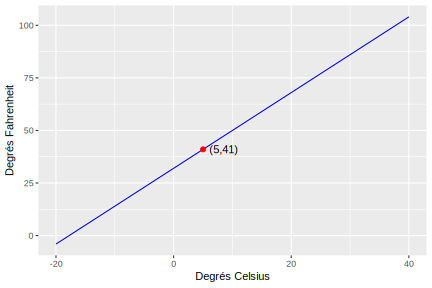
\includegraphics[width=0.9\linewidth]{algebre1_files/figure-latex/celsius-fahrenheit-1} 

}

\caption{L'équation linéaire permettant de convertir des degrés Celsius en degrés Fahrenheit.}\label{fig:celsius-fahrenheit}
\end{figure}

Dans le cas où nous n'avons qu'une seule équation linéaire, nous verrons qu'il est relativement simple de résoudre ce type d'équations.

\BeginKnitrBlock{example}
\protect\hypertarget{exm:unnamed-chunk-10}{}{\label{exm:unnamed-chunk-10} }Résolvez les équations linéaires suivantes:

\begin{enumerate}
\def\labelenumi{\alph{enumi}.}
\tightlist
\item
  \(3x+1=4\)
\item
  \(F=\dfrac{9}{5}C+32\)
\item
  \(2x_1+x_2-3x_3-5=0\)
\end{enumerate}
\EndKnitrBlock{example}

\hypertarget{systeme_equation_lineaire}{%
\section{Les systèmes d'équations linéaires}\label{systeme_equation_lineaire}}

Il semble donc qu'il soit simple de résoudre une seule équation linéaire, peu importe le nombre de variables. Par contre, en pratique, nous rencontrons la plupart du temps des systèmes d'équations linéaires, c'est-à-dire un ensemble d'équations linéaires.

\BeginKnitrBlock{example}[Un système d'équations linéaires chinois du troisième siècle avant notre ère]
\protect\hypertarget{exm:chinois}{}{\label{exm:chinois} \iffalse (Un système d'équations linéaires chinois du troisième siècle avant notre ère) \fi{} }Voici un exemple de système d'équations linéaires:
\begin{align*}
\begin{array}{cccccccc}
&3x&+&2y&+&z&=&39\\
&2x&+&3y&+&z&=&34\\
&x&+&2y&+&3z&=&26\\
\end{array}
\end{align*}
Ce système et sa solution se trouvent dans un livre chinois de mathématiques du troisième siècle avant notre ère. Vérifiez que
\begin{align*}
    x = \frac{37}{4},\quad y = \frac{17}{4},\quad z = \frac{11}{4}
\end{align*}
est une solution du système d'équations linéaires précédent.
\EndKnitrBlock{example}

Comme l'exemple précédent le démontre, il est simple de vérifier qu'un \(n\)-uplet forme une solution d'un système d'équations linéaires. Il sera par contre plus difficile de le trouver.

\BeginKnitrBlock{definition}[Un système d'équations linéaires]
\protect\hypertarget{def:unnamed-chunk-11}{}{\label{def:unnamed-chunk-11} \iffalse (Un système d'équations linéaires) \fi{} }Un \textbf{système d'équations linéaires} \(S\) de \(m\) équations et \(n\) variables (ou inconnues) \(x_1\), \(x_2\), \ldots{} et \(x_n\) est un ensemble de \(m\) équations linéaires de la forme:
\begin{align*}
S=\left\{\begin{array}{cccccccccc}
&a_{1,1}x_1&+&a_{1,2}x_2&+&\ldots &+&a_{1,n}x_n&=&b_1 \\
&a_{2,1}x_1&+&a_{2,2}x_2&+&\ldots &+&a_{2,n}x_n&=&b_2 \\
&&&&&&&&\vdots & \\
&a_{m,1}x_1&+&a_{m,2}x_2&+&\ldots &+&a_{m,n}x_n&=&b_m
\end{array}
\right.
\end{align*}
Les nombres \(a_{1,1}\), \(a_{1,2}\), \ldots{}, \(a_{1,n}\), \(a_{2,1}\), \ldots{}, \(a_{2,n}\), \ldots{}, \(a_{m,1}\), \ldots{}, \(a_{m,n}\) sont les \textbf{coefficients} du système et \(b_1\), \(b_2\), \ldots{}, \(b_m\) sont les \textbf{termes constants}. Si les termes constants sont tous zéros, le système est appelé \textbf{homogène}. Le système homogène qui possède les mêmes coefficients que le système ci-haut est dit être \textbf{associé} au système ci-haut.
\EndKnitrBlock{definition}

\BeginKnitrBlock{definition}[La solution d'un système  d'équations linéaires]
\protect\hypertarget{def:unnamed-chunk-12}{}{\label{def:unnamed-chunk-12} \iffalse (La solution d'un système d'équations linéaires) \fi{} }Une \textbf{solution} d'un système d'équations linéaires de \(m\) équations et de \(n\) variables
est un \(n\)-uplet écrit sous la forme \(r_1,r_2,...,r_n\) (qui veut dire \(x_1=r_1\), \(x_2=r_2\),\ldots{} et \(x_n=r_n\)), qui vérifie les \(m\) équations du système.
\EndKnitrBlock{definition}

\BeginKnitrBlock{definition}[L'ensemble solution d'un système  d'équations linéaires]
\protect\hypertarget{def:unnamed-chunk-13}{}{\label{def:unnamed-chunk-13} \iffalse (L'ensemble solution d'un système d'équations linéaires) \fi{} }L'\textbf{ensemble solution} d'un système d'équations linéaires est l'ensemble de toutes les solutions possibles du système. Nous le notons par \(ES\).
\EndKnitrBlock{definition}

Il existe trois types de solutions pour un système d'équations linéaires.

\BeginKnitrBlock{theorem}[Les types de solutions d'un système d'équations linéaires]
\protect\hypertarget{thm:unnamed-chunk-14}{}{\label{thm:unnamed-chunk-14} \iffalse (Les types de solutions d'un système d'équations linéaires) \fi{} }Les types de solutions d'un système d'équations linéaires sont:

\begin{itemize}
\tightlist
\item
  Une solution unique, c'est-à-dire qu'il existe un unique \(n\)-uplet qui soit solution du système d'équations linéaires.
\item
  Aucune solution, c'est-à-dire qu'il n'existe aucun \(n\)-uplet qui soit solution du système d'équations linéaires.
\item
  Une infinité de solutions, c'est-à-dire qu'il existe une infinité de \(n\)-uplet qui sont solutions du système d'équations linéaires.
\end{itemize}
\EndKnitrBlock{theorem}

\begin{figure}

{\centering 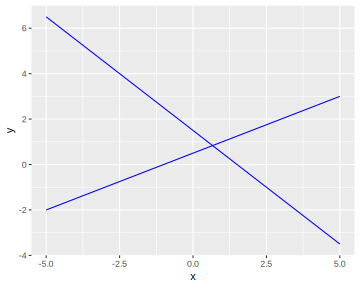
\includegraphics[width=0.33\linewidth]{algebre1_files/figure-latex/unnamed-chunk-15-1} 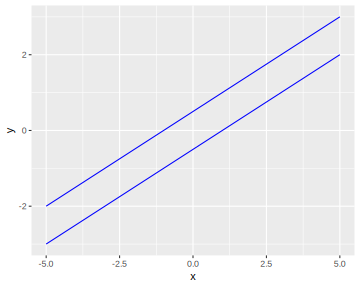
\includegraphics[width=0.33\linewidth]{algebre1_files/figure-latex/unnamed-chunk-15-2} 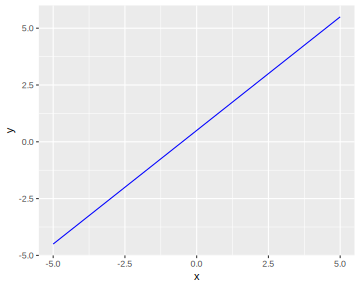
\includegraphics[width=0.33\linewidth]{algebre1_files/figure-latex/unnamed-chunk-15-3} 

}

\caption{Les trois types de solutions d'un système d'équations linéaires}\label{fig:unnamed-chunk-15}
\end{figure}

Il est possible d'abréger l'écriture d'un système d'équations linéaires en ne conservant que les coefficients et les constantes de ce système, en supposant que le nom et l'ordre des variables a été spécifié. Cette façon de représenter un système d'équations linéaires est appelé la matrice augmentée du système.

\BeginKnitrBlock{definition}[La matrice augmentée d'un système d'équations linéaires]
\protect\hypertarget{def:unnamed-chunk-16}{}{\label{def:unnamed-chunk-16} \iffalse (La matrice augmentée d'un système d'équations linéaires) \fi{} }Soit un système d'équations linéaires de la forme suivante:
\begin{align*}
\begin{array}{cccccccccc}
&a_{1,1}x_1&+&a_{1,2}x_2&+&\ldots &+&a_{1,n}x_n&=&b_1 \\
&a_{2,1}x_1&+&a_{2,2}x_2&+&\ldots &+&a_{2,n}x_n&=&b_2 \\
&&&&&&&&\vdots & \\
&a_{m,1}x_1&+&a_{m,2}x_2&+&\ldots &+&a_{m,n}x_n&=&b_m
\end{array}
\end{align*}
La \textbf{matrice augmentée} de ce système est représentée par l'arrangement rectangulaire suivant:
\begin{align*}
\left[\begin{array}{cccc|c}
a_{1,1}&a_{1,2}&\ldots &a_{1,n}&b_1 \\
a_{2,1}&a_{2,2}&\ldots &a_{2,n}&b_2 \\
\vdots &\vdots &&\vdots & \vdots \\
a_{m,1}&a_{m,2}&\ldots &a_{m,n}&b_m
\end{array}\right]
\end{align*}
Les coefficients sont placés en ordre à gauche de la barre verticale et les constantes sont placées à droite de la barre verticale. Cette barre symbolise l'égalité et permet de séparer visuellement les coefficients des constantes.
\EndKnitrBlock{definition}

\hypertarget{systeme-equation-lineaire-echelonnee}{%
\section{La résolution de système d'équations linéaires échelonnés}\label{systeme-equation-lineaire-echelonnee}}

Nous savons maintenant comment vérifier si les éléments d'un ensemble forme une solution d'un système d'équations linéaires. Nous ne savons par contre pas comment les trouver.

Par contre, avant d'apprendre des méthodes générales pour résoudre des systèmes d'équations linéaires, nous allons étudier quelques formes particulières de système d'équations linéaires qui se résolvent facilement. Nous en profiterons également pour mettre en lien ces systèmes avec leurs différents types de solutions.

Les systèmes les plus simples à résoudre sont ceux que nous rencontrons sous une forme échelonnée ou une forme échelonnée réduite.

\BeginKnitrBlock{definition}
\protect\hypertarget{def:unnamed-chunk-17}{}{\label{def:unnamed-chunk-17} }Un système d'équations linéaires est dit être sous la \textbf{forme échelonnée} si les conditions suivantes sont remplies:

\begin{itemize}
\tightlist
\item
  Toutes les lignes non-nulles, c'est-à-dire les lignes qui possèdent au moins un élément différent de zéro, se trouvent au-dessus des lignes nulles, c'est-à-dire des lignes qui ne possèdent que des zéros.
\item
  Le premier élément non-nul d'une ligne, c'est-à-dire le premier élément différent de zéro en partant de la gauche sur la ligne, est toujours situé à droite du premier élément non-nul de la ligne située au-dessus. Nous disons que le premier élément non-nul d'une ligne est le \textbf{pivot} de cette ligne.
\item
  Tous les éléments de la colonne situés sous un pivot sont composés de zéros.
\end{itemize}

Un système d'équations linéaires est dit être sous la \textbf{forme échelonnée réduite} s'il est déjà sous la forme échelonnée et si les conditions suivantes sont remplies:

\begin{itemize}
\tightlist
\item
  Le pivot d'une ligne est le seul élément non-nul de la colonne où il se situe.
\item
  Tous les pivots sont \(1\).
\end{itemize}
\EndKnitrBlock{definition}

La présente section présente la façon de résoudre des systèmes d'équations linéaires sous forme échelonnée, c'est-à-dire un système composé de \(m\) équations et de \(n\) inconnues.
\begin{align*}
\begin{array}{cccccccccc}
a_{1,1}x_1 & +& a_{1,2}x_2 & +&  a_{1,3}x_3 & \ldots & +&  a_{1,n}x_n & =& b_1  \\
        & & a_{2,2}x_2 & +&  a_{2,3}x_3 & \ldots & +& a_{2,n}x_n & =& b_2  \\
        & &         & &    & \ddots & & \vdots & =& \vdots   \\
%         & &         & &          & \ddots & & a_{n-1,n} & =& b_{n-1}\\
       & &         & &          &        & & a_{m,n}x_n & =& b_m
\end{array}
\end{align*}

Voici un exemple de matrice échelonnée:
\[ \begin{bmatrix}
\oplus & * & * & * & * & * & * & * & * \\
0 & 0 & \oplus & * & * & * & * & * & * \\
0 & 0 & 0 & \oplus & * & * & * & * & * \\ 
0 & 0 & 0 & 0 & 0 & 0 & \oplus & * & * \\ 
0 & 0 & 0 & 0 & 0 & 0 & 0 & 0 & \oplus \\ 
0 & 0 & 0 & 0 & 0 & 0 & 0 & 0 & 0 
\end{bmatrix} \]

La matrice échelonnée réduite associée à l'exemple précédent est:
\[\begin{bmatrix}
1 & * & 0 & 0 & * & * & 0 & * & 0 \\
0 & 0 & 1 & 0 & * & * & 0 & * & 0 \\
0 & 0 & 0 & 1 & * & * & 0 & * & 0 \\ 
0 & 0 & 0 & 0 & 0 & 0 & 1 & * & 0 \\ 
0 & 0 & 0 & 0 & 0 & 0 & 0 & 0 & 1 \\ 
0 & 0 & 0 & 0 & 0 & 0 & 0 & 0 & 0 
\end{bmatrix} \]

Un système d'équations linéaires sous la forme échelonnée se résout lui aussi assez facilement à l'aide de la méthode dite de ``substitution arrière''. La méthode tient son nom du fait que nous commençons à résoudre l'équation située à la dernière ligne. Nous substituons ensuite la valeur trouvée dans l'équation précédente pour résoudre cette équation et nous répétons jusqu'à l'équation située sur la première ligne.

\BeginKnitrBlock{example}
\protect\hypertarget{exm:unnamed-chunk-18}{}{\label{exm:unnamed-chunk-18} }Trouvez l'ensemble solution des systèmes d'équations linéaires suivants, présentés sous la forme échelonnée.

\begin{enumerate}
\def\labelenumi{\alph{enumi}.}
\tightlist
\item
  \begin{align*}
  \begin{array}{cccccccc}
  &-10x&+&5y&-&7z&=&40 \\
  &&&y&+&z&=&-12 \\
  &&&&&3z&=&0
  \end{array}
  \end{align*}
\item
  \begin{align*}
  \begin{array}{cccccccccc}
  &-x_{1}&-&4x_{2}&-&2x_{3}&-&x_{4}&=&-4\\
  &&&&&5x_{3}&+&2x_{4}&=&3\\
  &&&&&&&x_{4}&=&-1\\
  \end{array}
  \end{align*}
\item
  \begin{align*}
  \left[\begin{array}{ccc|c}
  7&-4&-2&-9\\
  0&-19&22&-62\\
  0&0&196&826\\
  0&0&0&133\\
  \end{array}\right]
  \end{align*}
\end{enumerate}
\EndKnitrBlock{example}

\hypertarget{methode-gauss}{%
\section{La méthode d'élimination de Gauss}\label{methode-gauss}}

Nous avons vu dans la section précédente comment résoudre des systèmes d'équations linéaires sous forme échelonnée ou sous forme échelonnée réduite. Dans cette section, nous voulons voir de quelle façon il est possible de transformer tout système d'équations linéaires sous l'une de ces deux formes.

Pour être en mesure de transformer un système d'équations linéaires, nous allons avoir besoin de connaître les opérations qui permettent de modifier des équations linéaires tout en conservant le même ensemble solution.

\BeginKnitrBlock{definition}[Systèmes d'équations linéaires équivalents]
\protect\hypertarget{def:unnamed-chunk-19}{}{\label{def:unnamed-chunk-19} \iffalse (Systèmes d'équations linéaires équivalents) \fi{} }Deux systèmes d'équations linéaires \(S_1\) et \(S_2\) sont dits \textbf{équivalents} s'ils possèdent le même ensemble solution. Nous notons alors \(S_1\sim S_2\).
\EndKnitrBlock{definition}

Les opérations élémentaires sur les équations vont permettre de modifier le système d'équations linéaires en un système équivalent, notamment sous la forme d'un système échelonné.

\BeginKnitrBlock{definition}[Opérations élémentaires sur les équations linéaires]
\protect\hypertarget{def:unnamed-chunk-20}{}{\label{def:unnamed-chunk-20} \iffalse (Opérations élémentaires sur les équations linéaires) \fi{} }Soit \(L_i\) la ième équation d'un système d'équations linéaires. Les \textbf{opérations élémentaires sur les équations linéaires} sont les suivantes:

\begin{itemize}
\tightlist
\item
  Nous pouvons additionner ou soustraire deux équations: \(L_i \pm L_j \rightarrow L_i\)
\item
  Nous pouvons multiplier une équation par une constante non-nulle: \(kL_i \rightarrow L_i\)
\item
  Nous pouvons intervertir deux équations: \(L_i \leftrightarrow L_j\)
\end{itemize}
\EndKnitrBlock{definition}

\BeginKnitrBlock{theorem}
\protect\hypertarget{thm:unnamed-chunk-21}{}{\label{thm:unnamed-chunk-21} }Les trois opérations élémentaires sur les équations linéaires ne changent pas l'ensemble solution du système d'équations linéaires.
\EndKnitrBlock{theorem}

\BeginKnitrBlock{proposition}
\protect\hypertarget{prp:unnamed-chunk-22}{}{\label{prp:unnamed-chunk-22} }L'opération
\begin{align*}
k_1L_i+k_2L_j \rightarrow L_i
\end{align*}
avec \(i\neq j\) et \(k_1,k_2\in\mathbb{R}\setminus \{0\}\) n'affecte pas l'ensemble solution du système d'équations linéaires.
\EndKnitrBlock{proposition}

Maintenant, nous voulons utiliser les opérations élémentaires sur les lignes pour transformer la matrice augmentée sous la forme échelonnée. C'est ce que nous nommons \textbf{la méthode de Gauss}.

\BeginKnitrBlock{example}
\protect\hypertarget{exm:unnamed-chunk-23}{}{\label{exm:unnamed-chunk-23} }Résolvez le système d'équations linéaires de l'exemple \ref{exm:chinois} à l'aide de la méthode de Gauss.
\begin{align*}
\begin{array}{cccccccc}
&3x&+&2y&+&z&=&39\\
&2x&+&3y&+&z&=&34\\
&x&+&2y&+&3z&=&26\\
\end{array}
\end{align*}
\EndKnitrBlock{example}

\BeginKnitrBlock{example}
\protect\hypertarget{exm:unnamed-chunk-24}{}{\label{exm:unnamed-chunk-24} }Résolvez le système d'équations linéaires suivant à l'aide de la méthode de Gauss.
\begin{align*}
\begin{array}{cccccccc}
&3x&-&7y&+&4z&=&34\\
&-6x&-&2y&+&9z&=&49\\
&7x&-&2y&-&5z&=&-21\\
\end{array}
\end{align*}
\EndKnitrBlock{example}

Il est parfois possible que nous devions interchanger deux lignes pour obtenir une matrice sous forme échelonnée. L'exemple suivant permettra de montrer comment faire.

\BeginKnitrBlock{example}
\protect\hypertarget{exm:unnamed-chunk-25}{}{\label{exm:unnamed-chunk-25} }Résolvez le système d'équations linéaires suivant.
\begin{align*}
\begin{array}{cccccccc}
&&&3y&-&4z&=&-31\\
&2x&-&y&+&2z&=&17\\
&3x&+&2y&-&5z&=&-24\\
\end{array}
\end{align*}
\EndKnitrBlock{example}

Nous obtenons parfois une infinité de solutions à notre système d'équations linéaires.

\BeginKnitrBlock{example}
\protect\hypertarget{exm:unnamed-chunk-26}{}{\label{exm:unnamed-chunk-26} }Résolvez le système d'équations linéaires suivant:
\begin{align*}
\begin{array}{cccccccc}
&4x&+&3y&-&8z&=&14\\
&-x&-&y&+&3z&=&-4\\
&5x&-&2y&+&13z&=&6\\
\end{array}
\end{align*}
\EndKnitrBlock{example}

Nous obtenons parfois aucune solution à notre système d'équations linéaires.

\BeginKnitrBlock{example}
\protect\hypertarget{exm:unnamed-chunk-27}{}{\label{exm:unnamed-chunk-27} }Résolvez le système d'équations linéaires suivant:
\begin{align*}
\begin{array}{cccccccc}
&-7x&-&4y&-&6z&=&-1\\
&17x&+&8y&+&15z&=&-8\\
&-7x&-&16y&-&3z&=&3\\
\end{array}
\end{align*}
\EndKnitrBlock{example}

\hypertarget{une-application}{%
\subsection{Une application}\label{une-application}}

\BeginKnitrBlock{example}
\protect\hypertarget{exm:plaque2d}{}{\label{exm:plaque2d} }La distribution de la chaleur à long terme dans une plaque de métal de forme carrée dont les côtés sont tenus à une certaine température constante peut être étudiée à l'aide d'une grille où chaque point est à la même distance que ses voisins. En première approximation, la chaleur à long terme en chaque point de cette grille est donnée par la température moyenne de ses voisins. Déterminez la température en chacun des points de la plaque suivante:
\EndKnitrBlock{example}

\begin{figure}

{\centering \includegraphics[width=0.75\linewidth]{algebre1_files/figure-latex/unnamed-chunk-28-1} 

}

\caption{Plaque chauffée.}\label{fig:unnamed-chunk-28}
\end{figure}

Pour obtenir une meilleure précision dans nos calculs, nous pourrions raffiner notre grille, c'est-à-dire lui ajouter des points. Par exemple, si nous prenons une grille \(5\times 5\),
nous obtenons le système d'équations linéaires présenté sous la forme d'une matrice augmentée suivant:
\[
\left[
\begin{smallmatrix}
4&-1&0&0&0&-1&0&0&0&0&0&0&0&0&0&0&0&0&0&0&0&0&0&0&0&250\\
-1&4&-1&0&0&0&-1&0&0&0&0&0&0&0&0&0&0&0&0&0&0&0&0&0&0&140\\
0&-1&4&-1&0&0&0&-1&0&0&0&0&0&0&0&0&0&0&0&0&0&0&0&0&0&140\\
0&0&-1&4&-1&0&0&0&-1&0&0&0&0&0&0&0&0&0&0&0&0&0&0&0&0&140\\
0&0&0&-1&4&0&0&0&0&-1&0&0&0&0&0&0&0&0&0&0&0&0&0&0&0&260\\
-1&0&0&0&0&4&-1&0&0&0&-1&0&0&0&0&0&0&0&0&0&0&0&0&0&0&110\\
0&-1&0&0&0&-1&4&-1&0&0&0&-1&0&0&0&0&0&0&0&0&0&0&0&0&0&0\\
0&0&-1&0&0&0&-1&4&-1&0&0&0&-1&0&0&0&0&0&0&0&0&0&0&0&0&0\\
0&0&0&-1&0&0&0&-1&4&-1&0&0&0&-1&0&0&0&0&0&0&0&0&0&0&0&0\\
0&0&0&0&-1&0&0&0&-1&4&0&0&0&0&-1&0&0&0&0&0&0&0&0&0&0&120\\
0&0&0&0&0&-1&0&0&0&0&4&-1&0&0&0&-1&0&0&0&0&0&0&0&0&0&110\\
0&0&0&0&0&0&-1&0&0&0&-1&4&-1&0&0&0&-1&0&0&0&0&0&0&0&0&0\\
0&0&0&0&0&0&0&-1&0&0&0&-1&4&-1&0&0&0&-1&0&0&0&0&0&0&0&0\\
0&0&0&0&0&0&0&0&-1&0&0&0&-1&4&-1&0&0&0&-1&0&0&0&0&0&0&0\\
0&0&0&0&0&0&0&0&0&-1&0&0&0&-1&4&0&0&0&0&-1&0&0&0&0&0&120\\
0&0&0&0&0&0&0&0&0&0&-1&0&0&0&0&4&-1&0&0&0&-1&0&0&0&0&110\\
0&0&0&0&0&0&0&0&0&0&0&-1&0&0&0&-1&4&-1&0&0&0&-1&0&0&0&0\\
0&0&0&0&0&0&0&0&0&0&0&0&-1&0&0&0&-1&4&-1&0&0&0&-1&0&0&0\\
0&0&0&0&0&0&0&0&0&0&0&0&0&-1&0&0&0&-1&4&-1&0&0&0&-1&0&0\\
0&0&0&0&0&0&0&0&0&0&0&0&0&0&-1&0&0&0&-1&4&0&0&0&0&-1&120\\
0&0&0&0&0&0&0&0&0&0&0&0&0&0&0&-1&0&0&0&0&4&-1&0&0&0&240\\
0&0&0&0&0&0&0&0&0&0&0&0&0&0&0&0&-1&0&0&0&-1&4&-1&0&0&130\\
0&0&0&0&0&0&0&0&0&0&0&0&0&0&0&0&0&-1&0&0&0&-1&4&-1&0&130\\
0&0&0&0&0&0&0&0&0&0&0&0&0&0&0&0&0&0&-1&0&0&0&-1&4&-1&130\\
0&0&0&0&0&0&0&0&0&0&0&0&0&0&0&0&0&0&0&-1&0&0&0&-1&4&250\\
\end{smallmatrix}
\right]
\]
Comme nous pouvons le constater, le système d'équations linéaires devient rapidement beaucoup trop grand pour le résoudre ``à la main''. Nous allons donc utiliser un logiciel de calcul pour le résoudre.

\begin{figure}

{\centering \includegraphics[width=0.75\linewidth]{algebre1_files/figure-latex/unnamed-chunk-29-1} 

}

\caption{Plaque chauffée.}\label{fig:unnamed-chunk-29}
\end{figure}

La figure suivante présente le même problème étudié précédemment, mais sur une grille \(50\times 50\).

\begin{center}\includegraphics[width=0.75\linewidth]{resources/images/grille_chaleur} \end{center}

\hypertarget{les-systuxe8mes-duxe9quations-linuxe9aires-homoguxe8nes}{%
\section{Les systèmes d'équations linéaires homogènes}\label{les-systuxe8mes-duxe9quations-linuxe9aires-homoguxe8nes}}

Les systèmes d'équations linéaires homogènes sont une classe particulière de systèmes d'équations linéaires. Ceux-ci ont la particularité de toujours posséder au moins une solution. Il est impossible qu'un tel système ne possède aucune solution.

\BeginKnitrBlock{definition}[Un système d'équations linéaires homogène]
\protect\hypertarget{def:unnamed-chunk-31}{}{\label{def:unnamed-chunk-31} \iffalse (Un système d'équations linéaires homogène) \fi{} }Un \textbf{système d'équations linéaires homogène} de \(m\) équations et \(n\) variables (ou inconnues) \(x_1\), \(x_2\), \ldots{} et \(x_n\) est un ensemble de \(m\) équations linéaires de la forme:
\begin{align*}
\begin{array}{cccccccccc}
&a_{1,1}x_1&+&a_{1,2}x_2&+&\ldots &+&a_{1,n}x_n&=&0 \\
&a_{2,1}x_1&+&a_{2,2}x_2&+&\ldots &+&a_{2,n}x_n&=&0 \\
&&&&&&&&\vdots & \\
&a_{m,1}x_1&+&a_{m,2}x_2&+&\ldots &+&a_{m,n}x_n&=&0
\end{array}
\end{align*}
La matrice augmentée d'un tel système est:
\begin{align*}
\left[\begin{array}{cccc|c}
a_{1,1}&a_{1,2}&\ldots &a_{1,n}&0 \\
a_{2,1}&a_{2,2}&\ldots &a_{2,n}&0 \\
\vdots &\vdots &&\vdots & \vdots \\
a_{m,1}&a_{m,2}&\ldots &a_{m,n}&0
\end{array}\right]
\end{align*}
\EndKnitrBlock{definition}

Un système d'équations linéaires homogène possède toujours une solution. En effet, la solution triviale \(x_1=x_2=\ldots=x_n=0\) forme toujours une solution d'un système. Puisqu'il est impossible que le système ne possède aucune solution, il possède soit une solution unique (la solution triviale) soit une infinité de solutions.

\BeginKnitrBlock{example}
\protect\hypertarget{exm:unnamed-chunk-32}{}{\label{exm:unnamed-chunk-32} }Déterminez les valeurs de \(a\), \(b\), \(c\) et \(d\) qui équilibrent l'équation chimique suivante:
\begin{align*}
aC_2H_6+bO_2 \rightarrow cCO_2+dH_2O
\end{align*}
\EndKnitrBlock{example}

\hypertarget{une-application-1}{%
\subsection{Une application}\label{une-application-1}}

\BeginKnitrBlock{example}
\protect\hypertarget{exm:unnamed-chunk-33}{}{\label{exm:unnamed-chunk-33} }La loi des leviers d'Archimède stipule que deux masses sont en équilibre sur une balance si leurs poids sont inversement proportionnels à leur distance par rapport au point d'appui. En d'autres mots, pour que deux masses \(m_1\) et \(m_2\) situées respectivement à des distances \(d_1\) et \(d_2\) du point d'appui soient en équilibre, il faut que:
\begin{align*}
    m_1d_1 &= m_2d_2
\end{align*}
Trouvez les masses \(m_1\), \(m_2\), \(m_3\) et \(m_4\) pour que le système suivant soit en équilibre.
\EndKnitrBlock{example}

\begin{figure}

{\centering \includegraphics[width=0.75\linewidth]{algebre1_files/figure-latex/unnamed-chunk-34-1} 

}

\caption{La loi des leviers d'Archimède.}\label{fig:unnamed-chunk-34}
\end{figure}

\hypertarget{la-muxe9thode-de-gauss-avec-substitution-arriuxe8re}{%
\section{La méthode de Gauss avec substitution arrière}\label{la-muxe9thode-de-gauss-avec-substitution-arriuxe8re}}

La section précédente nous a permis d'introduire la méthode d'élimination de Gauss. Celle-ci permettait d'obtenir une matrice sous forme échelonnée. Une fois cette matrice obtenue, il nous était possible d'utiliser la méthode de substitution arrière pour trouver l'ensemble solution du système d'équations linéaires. Dans cette section, nous introduirons la méthode d'élimination de Gauss avec substitution arrière, c'est-à-dire que nous obtiendrons une matrice échelonnée réduite en effectuant la méthode de Gauss et ensuite la méthode de substitution arrière directement sur la matrice augmentée.

\BeginKnitrBlock{example}
\protect\hypertarget{exm:unnamed-chunk-35}{}{\label{exm:unnamed-chunk-35} }Résolvez le système d'équations linéaires suivant à l'aide de la méthode de Gauss avec substitution arrière.
\begin{align*}
\begin{array}{cccccccc}
&-4x&+&5y&+&z&=&9\\
&3x&&&+&5z&=&-19\\
&3x&+&5y&-&4z&=&98\\
&4x&-&5y&+&5z&=&-57\\
\end{array}
\end{align*}
\EndKnitrBlock{example}

\BeginKnitrBlock{example}
\protect\hypertarget{exm:unnamed-chunk-36}{}{\label{exm:unnamed-chunk-36} }Résolvez le système d'équations linéaires suivant:
\begin{align*}
\begin{array}{cccccccccc}
&-2w&-&3x&+&5y&-&2z&=&0\\
&4w&+&2x&-&3y&-&2z&=&4\\
&14w&+&x&&&-&16z&=&10\\
\end{array}
\end{align*}
\EndKnitrBlock{example}

\BeginKnitrBlock{example}
\protect\hypertarget{exm:unnamed-chunk-37}{}{\label{exm:unnamed-chunk-37} }Résolvez le système d'équations linéaires suivant:
\begin{align*}
\begin{array}{cccccccccc}
&-2x_{1}&-&3x_{2}&+&4x_{3}&-&20x_{4}&=&15\\
&x_{1}&-&3x_{2}&-&2x_{3}&-&8x_{4}&=&6\\
&x_{1}&&&-&2x_{3}&+&4x_{4}&=&-3\\
\end{array}
\end{align*}
\EndKnitrBlock{example}

\hypertarget{une-application-2}{%
\subsection{Une application}\label{une-application-2}}

\BeginKnitrBlock{example}
\protect\hypertarget{exm:unnamed-chunk-38}{}{\label{exm:unnamed-chunk-38} }Trouvez l'équation de la parabole passant par les points \(P(1,6)\), \(Q(-3,34)\) et \(R(2,9)\).
\EndKnitrBlock{example}

\hypertarget{matrices}{%
\chapter{Les matrices}\label{matrices}}

\BeginKnitrBlock{example}[Les photos en niveaux de gris]
\protect\hypertarget{exm:unnamed-chunk-39}{}{\label{exm:unnamed-chunk-39} \iffalse (Les photos en niveaux de gris) \fi{} }Une image digitale en niveaux de gris peut être représentée mathématiquement par une matrice. Les éléments de la matrice sont des nombres situés dans l'intervalle \(0\) (qui représente la couleur noire) et \(255\) (qui représente la couleur blanche). Chaque entrée de la matrice peut être visualisée comme un petit carré coloré d'un niveau de gris constant qui dépend de la valeur de l'entrée. Nous appelons ces petits carrés des pixels; ils sont facilement reconnaissables lorsque nous faisons un zoom sur une image.

Par exemple, dans la figure \ref{fig:baboon}, nous avons encadré un carré de dimension \(16\times 16\) sur le museau du mandrill. La matrice située sous l'image correspond à l'intensité des niveaux de gris à l'intérieur de ce carré.

\begin{align*}
\left[
\begin{array}{cccccccccccccccc}
168&162&168&173&168&160&170&162&135&92&129&152&145&161&173&175\\
168&173&176&179&172&169&157&154&136&100&133&149&147&162&175&176\\
156&167&170&174&163&152&154&152&138&128&96&120&144&166&169&167\\
177&182&176&175&178&177&166&167&143&136&108&106&135&165&160&167\\
167&171&160&151&178&182&171&145&143&159&136&103&136&148&159&168\\
165&175&178&165&157&162&175&179&157&151&149&124&111&143&162&169\\
166&152&159&165&158&161&166&174&177&166&151&160&120&138&162&163\\
176&174&171&181&176&170&162&166&168&180&169&155&135&109&156&153\\
167&175&172&171&174&167&174&178&173&178&182&168&139&112&144&157\\
173&173&175&179&173&170&174&182&179&169&165&168&165&143&118&145\\
174&174&178&178&180&171&169&169&172&162&164&156&146&154&106&132\\
172&172&175&172&181&181&179&183&183&177&180&172&145&136&121&102\\
171&176&177&179&175&175&175&181&180&168&162&171&169&161&142&117\\
176&177&176&178&176&177&176&173&177&181&175&160&178&180&170&153\\
162&166&166&171&175&169&180&186&185&173&182&164&158&170&161&143\\
173&170&165&173&178&169&158&168&180&179&176&176&167&170&171&161\\
\end{array}\right]
\end{align*}
\EndKnitrBlock{example}

\begin{figure}

{\centering \includegraphics[width=0.5\linewidth]{resources/images/baboon} 

}

\caption{Une image d'un mandrill.}\label{fig:baboon}
\end{figure}

\BeginKnitrBlock{example}[Les photos numériques]
\protect\hypertarget{exm:unnamed-chunk-40}{}{\label{exm:unnamed-chunk-40} \iffalse (Les photos numériques) \fi{} }Les écrans de nos téléphones intelligents sont formés de pixels rouge, vert et bleu.

Rouge, vert, bleu, abrégé en RVB ou en RGB (de l'anglais « red, green, blue ») est un système de codage informatique des couleurs, le plus proche du matériel. Les écrans d'ordinateurs reconstituent une couleur par synthèse additive à partir de trois couleurs primaires, un rouge, un vert et un bleu, formant sur l'écran une mosaïque trop petite pour être aperçue. Le codage RVB indique une valeur pour chacune de ces couleurs primaires.
\EndKnitrBlock{example}

\begin{figure}

{\centering \includegraphics[width=0.5\linewidth]{resources/images/pixels} 

}

\caption{Quelques exemples de pixels agrandis.}\label{fig:unnamed-chunk-41}
\end{figure}

Voici un exemple du principe d'utilisation des pixels rouge, vert et bleu: \href{https://docs.google.com/spreadsheets/d/e/2PACX-1vQlMpjcuG6vAjO40W1oMXe3J40wmDczGQEHzdvz1aHF_HadCymBE_OS-f197cYWvoGnnmqERiR7aKkw/pubhtml}{une feuille de calcul pas comme les autres}.

Voici aussi un sketch d'un humoriste portant sur les \href{https://www.youtube.com/watch?v=UBX2QQHlQ_I}{feuilles de calcul}.

\hypertarget{la-duxe9finition-dune-matrice}{%
\section{La définition d'une matrice}\label{la-duxe9finition-dune-matrice}}

Débutons en introduisant la définition d'une matrice. Nous avons déjà rencontré une matrice que nous avions nommé la matrice augmentée lors de la résolution de système d'équations linéaires.

\BeginKnitrBlock{definition}[Une matrice]
\protect\hypertarget{def:unnamed-chunk-42}{}{\label{def:unnamed-chunk-42} \iffalse (Une matrice) \fi{} }Une matrice \(A\) de dimension \(m \times n\) où \(m\) et \(n\) sont des entiers positifs est un arrangement de \(m\cdot n\) nombres sous la forme de \(m\) lignes horizontales et de \(n\) colonnes verticales. Nous notons habituellement une matrice à l'aide d'une lettre majuscule et nous encadrons les nombres formant la matrice à l'aide de crochets. Nous avons donc:
\begin{align*}
A = \begin{bmatrix}
a_{1,1}&a_{1,2}&\ldots &a_{1,n} \\
a_{2,1}&a_{2,2}&\ldots &a_{2,n}\\
\vdots &\vdots & \ddots &\vdots \\
a_{m,1}&a_{m,2}&\ldots &a_{m,n}
\end{bmatrix}
\end{align*}

Le nombre \(a_{i,j}\) correspond à l'entrée \((i,j)\) de la matrice \(A\), c'est-à-dire au nombre situé à l'intersection de la ième ligne et de la jième colonne. Remarquons que nous utilisons une lettre minuscule pour indiquer un nombre de la matrice.

La \emph{ième} ligne et la \emph{jième} colonne de la matrice \(A\) sont respectivement:
\begin{align*}
\begin{bmatrix}
a_{i,1} & a_{i,2} & \ldots & a_{i,n}
\end{bmatrix}
\quad 
\text{et}
\quad
\begin{bmatrix}
a_{1,j} \\
a_{2,j} \\
\vdots \\
a_{m,j}
\end{bmatrix}
\end{align*}

En particulier, nous disons qu'une matrice \(A\) de dimension \(1\times n\) est une matrice ligne et qu'une matrice \(A\) de dimension \(m\times 1\) est une matrice colonne.
\EndKnitrBlock{definition}

La figure \ref{fig:indices-matrice} présente le positionnement des indices dans une matrice.

\begin{figure}

{\centering \includegraphics[width=0.75\linewidth]{algebre1_files/figure-latex/indices-matrice-1} 

}

\caption{Le positionnement des indices dans une matrice.}\label{fig:indices-matrice}
\end{figure}

\BeginKnitrBlock{remark}
\iffalse{} {Remarque. } \fi{}Nous pouvons noter la dimension d'une matrice en utilisant des indices séparés par une virgule. Par exemple, si la matrice \(A\) est de dimension \(m \times n\), nous pouvons l'écrire des deux façons suivantes:
\begin{align*}
    A_{m\times n} \qquad \text{ou} \qquad [a_{i,j}]_{m\times n}
\end{align*}
\EndKnitrBlock{remark}

\BeginKnitrBlock{remark}
\iffalse{} {Remarque. } \fi{}Nous pouvons utiliser de grandes parenthèses comme notation lors de l'écriture d'une matrice, c'est-à-dire qu'une matrice \(A\) de dimension \(m \times n\) peut s'écrire:
\begin{align*}
A = \begin{pmatrix}
a_{1,1}&a_{1,2}&\ldots &a_{1,n} \\
a_{2,1}&a_{2,2}&\ldots &a_{2,n}\\
\vdots &\vdots & \ddots &\vdots \\
a_{m,1}&a_{m,2}&\ldots &a_{m,n}
\end{pmatrix}
\end{align*}
Par contre, dans ce manuel, nous utiliserons uniquement les crochets.
\EndKnitrBlock{remark}

\BeginKnitrBlock{example}
\protect\hypertarget{exm:unnamed-chunk-45}{}{\label{exm:unnamed-chunk-45} }Indiquez la dimension des matrices suivantes.

\begin{enumerate}
\def\labelenumi{\alph{enumi}.}
\tightlist
\item
  \(A = \begin{bmatrix}  10&10&6\\  10&10&-8\\  -7&0&-2\\  \end{bmatrix}\)
\item
  \(B = \begin{bmatrix}  9\\  6\\  10\\  3\\  -10\\  \end{bmatrix}\)
\item
  \(C = \begin{bmatrix}  7&9&4&5\\  \end{bmatrix}\)
\item
  \(D = \begin{bmatrix}  7\\  \end{bmatrix}\)
\item
  \(E = \begin{bmatrix}  9&3&1&-7&0\\  -8&-8&10&10&6\\  9&-5&10&10&-8\\  \end{bmatrix}\)
\end{enumerate}
\EndKnitrBlock{example}

\BeginKnitrBlock{example}
\protect\hypertarget{exm:unnamed-chunk-46}{}{\label{exm:unnamed-chunk-46} }Soit la matrice suivante:
\begin{align*}
A = \begin{bmatrix}
-2&-10&5&-10\\
9&7&-2&-5\\
6&9&3&-10\\
10&4&-7&-8\\
3&5&4&7\\
\end{bmatrix}
\end{align*}
Répondez aux questions suivantes.

\begin{enumerate}
\def\labelenumi{\alph{enumi}.}
\tightlist
\item
  Déterminez la valeur de l'élément \(a_{1,2}\).
\item
  Déterminez la valeur de l'élément \(a_{2,1}\).
\item
  Déterminez la valeur de l'élément \(a_{3,3}\).
\item
  Déterminez la valeur de l'élément \(a_{4,5}\).
\end{enumerate}
\EndKnitrBlock{example}

\hypertarget{sec:matrice-particuliere}{%
\subsection{Les matrices particulières}\label{sec:matrice-particuliere}}

\BeginKnitrBlock{definition}[Une matrice carrée]
\protect\hypertarget{def:unnamed-chunk-47}{}{\label{def:unnamed-chunk-47} \iffalse (Une matrice carrée) \fi{} }Soit \(A\) une matrice. Nous disons que \(A\) est une matrice carrée si elle possède le même nombre de lignes que de colonnes, c'est-à-dire que nous pouvons écrire \(A_{m \times m}\).

En particulier, nous disons que les entrées \([a_{i,i}]_{m \times m}\) de la matrice forment la diagonale principale de la matrice. Par exemple, si nous avons la matrice \(A_{4\times 4}\) suivante:
\begin{align*}
A = \begin{bmatrix}
\fbox{$a_{1,1}$} & a_{1,2} & a_{1,3} & a_{1,4} \\
a_{2,1} & \fbox{$a_{2,2}$} & a_{2,3} & a_{2,4} \\
a_{3,1} & a_{3,2} & \fbox{$a_{3,3}$} & a_{3,4} \\
a_{4,1} & a_{4,2} & a_{4,3} & \fbox{$a_{4,4}$} \\
\end{bmatrix}
\end{align*}
les éléments encadrés, qui correspondent aux éléments appartenant à la ième ligne et à la ième colonne, sont les éléments de la diagonale principale.

Il existe également dans une matrice carrée, une diagonale secondaire. Nous disons que les entrées \([a_{m-i+1,i}]_{m \times m}\) (nous aurions aussi pu utiliser la notation \([a_{i,m-i+1}]_{m \times m}\)) de la matrice forment la diagonale secondaire de la matrice. Par exemple, si nous avons la matrice \(A_{4\times 4}\) suivante:
\begin{align*}
A = \begin{bmatrix}
a_{1,1} & a_{1,2} & a_{1,3} & \fbox{$a_{1,4}$} \\
a_{2,1} & a_{2,2} & \fbox{$a_{2,3}$} & a_{2,4} \\
a_{3,1} & \fbox{$a_{3,2}$} & a_{3,3} & a_{3,4} \\
\fbox{$a_{4,1}$} & a_{4,2} & a_{4,3} & a_{4,4} \\
\end{bmatrix}
\end{align*}
\EndKnitrBlock{definition}

\BeginKnitrBlock{definition}[Les matrices carrées usuelles]
\protect\hypertarget{def:matrice-usuelle}{}{\label{def:matrice-usuelle} \iffalse (Les matrices carrées usuelles) \fi{} }Voici quelques matrices carrées usuelles:

\begin{itemize}
\tightlist
\item
  La matrice identité, noté \(I_n\), est la matrice ne contenant que des uns sur sa diagonale principale et des zéros partout ailleurs. Par exemple, voici la matrice identité de format \(5 \times 5\):
  \begin{align*}
  I_5 &= \begin{bmatrix}
  1&0&0&0&0\\
  0&1&0&0&0\\
  0&0&1&0&0\\
  0&0&0&1&0\\
  0&0&0&0&1\\
  \end{bmatrix}
  \end{align*}
\item
  Une matrice diagonale est une matrice ne contenant que des zéros sauf sur la diagonale principale ou elle peut contenir des nombres différents de zéros. Par exemple, voici une matrice diagonale:
  \begin{align*}
  A = \begin{bmatrix}
  7&0&0&0\\
  0&9&0&0\\
  0&0&-8&0\\
  0&0&0&9\\
  \end{bmatrix}
  \end{align*}
  La matrice \(I_n\) est une matrice diagonale.
\item
  Une matrice triangulaire inférieure, notée \(L_n\), est une matrice telle que toutes les entrées au-dessus de la diagonale principale sont nulles. Mathématiquement, nous pouvons écrire:
  \begin{align*}
  [l_{i,j}]_n = \begin{cases}
  l_{i,j} & \text{si } i \geq j \\
  0 & \text{si } i < j
  \end{cases} 
  \end{align*}
  Nous pouvons représenter la matrice \(L_n\) de la façon suivante:
  \begin{align*}
  L_n &= \begin{bmatrix}
  l_{1,1} & & & & 0 \\
  l_{2,1} & l_{2,2} & & & \\
  l_{3,1} & l_{3,2} & \ddots & & \\
  \vdots & \vdots & \ddots & \ddots & \\
  l_{n,1} & l_{n,2} & \ldots & l_{n,n-1} & l_{n,n} 
  \end{bmatrix}
  \end{align*}
\item
  Une matrice triangulaire supérieure, notée \(U_n\), est une matrice telle que toutes les entrées au-dessous de la diagonale principale sont nulles. Mathématiquement, nous pouvons écrire:
  \begin{align*}
  [u_{i,j}]_n = \begin{cases}
  u_{i,j} & \text{si } i \leq j \\
  0 & \text{si } i > j
  \end{cases} 
  \end{align*}
  Nous pouvons représenter la matrice \(U_n\) de la façon suivante:
  \begin{align*}
  U_n &= \begin{bmatrix}
  u_{1,1} & u_{1,2} & u_{1,3} & \ldots & u_{1,n} \\
  & u_{2,2} & u_{2,3} & \ldots & u_{2,n} \\
  & & \ddots & \ddots & \vdots \\
  & & & \ddots & u_{n-1,n} \\
  0 & & & & u_{n,n}
  \end{bmatrix}
  \end{align*}
  Notons qu'une matrice sous forme échelonnée est une matrice triangulaire supérieure.
\item
  Une matrice symétrique est une matrice telle que \(a_{i,j}=a_{j,i}\) pour toutes les valeurs de \(i\) et de \(j\). Par exemple, les matrices suivantes sont symétriques:
  \begin{align*}
  A = \begin{bmatrix}
  a & b & c & d & e \\
  b & f & g & h & i \\
  c & g & j & k & l \\
  d & h & k & m & n \\
  e & i & l & n & o
  \end{bmatrix}
  \qquad
  B = \begin{bmatrix}
  2 & 4 & -5 \\
  4 & 0 & 3 \\
  -5 & 3 & 1
  \end{bmatrix}
  \end{align*}
\item
  Une matrice anti-symétrique est une matrice telle que \(a_{i,j}=-a_{j,i}\) pour toutes les valeurs de \(i\) et de \(j\). Par exemple, les matrices suivantes sont anti-symétriques:
  \begin{align*}
  A = \begin{bmatrix}
  0 & b & c & d & e \\
  -b & 0 & g & h & i \\
  -c & -g & 0 & k & l \\
  -d & -h & -k & 0 & n \\
  -e & -i & -l & -n & 0
  \end{bmatrix}
  \qquad
  B = \begin{bmatrix}
  0 & 4 & -5 \\
  -4 & 0 & 3 \\
  5 & -3 & 0
  \end{bmatrix}
  \end{align*}
\end{itemize}
\EndKnitrBlock{definition}

\BeginKnitrBlock{remark}
\iffalse{} {Remarque. } \fi{}La diagonale principale d'une matrice anti-symétrique n'est composée que de zéros.
\EndKnitrBlock{remark}

La dernière matrice que nous introduirons n'est pas une matrice carrée mais elle nous sera néanmoins très utile.

\BeginKnitrBlock{definition}[La matrice nulle]
\protect\hypertarget{def:unnamed-chunk-49}{}{\label{def:unnamed-chunk-49} \iffalse (La matrice nulle) \fi{} }La matrice nulle, notée \(O_{m\times n}\) est une matrice composée uniquement de zéros. Par exemple, les matrices suivantes sont des matrices nulles:
\begin{align*}
O_{2\times 2} = \begin{bmatrix}
0&0\\
0&0\\
\end{bmatrix}
\qquad 
O_{3,5} = \begin{bmatrix}
0&0&0&0&0\\
0&0&0&0&0\\
0&0&0&0&0\\
\end{bmatrix}
\end{align*}
\EndKnitrBlock{definition}

Les matrices que nous venons de décrire sont celles que nous utiliserons le plus régulièrement. Il existe par contre un très grand nombre de matrices particulières.

\hypertarget{les-opuxe9rations-matricielles}{%
\section{Les opérations matricielles}\label{les-opuxe9rations-matricielles}}

Dans cette section, nous allons introduire les opérations que nous pouvons effectuer sur les matrices.

Avant d'introduire les opérations matricielles, nous débuterons par indiquer les conditions que deux matrices doivent remplir pour être égales.

\BeginKnitrBlock{definition}[L'égalité entre deux matrices]
\protect\hypertarget{def:unnamed-chunk-50}{}{\label{def:unnamed-chunk-50} \iffalse (L'égalité entre deux matrices) \fi{} }Nous disons que deux matrices \(A=[a_{i,j}]_{m \times n}\) et \(B=[b_{i,j}]_{p \times q}\) sont égales si:

\begin{itemize}
\tightlist
\item
  \(A\) et \(B\) ont la même dimension, c'est-à-dire \(m=p\) et \(n=q\);
\item
  tous les éléments correspondants sont égaux, c'est-à-dire \(a_{i,j}=b_{i,j}\) pour tout \(i\) et \(j\).
\end{itemize}
\EndKnitrBlock{definition}

\BeginKnitrBlock{example}
\protect\hypertarget{exm:unnamed-chunk-51}{}{\label{exm:unnamed-chunk-51} }Déterminez si les matrices suivantes sont égales.
\begin{align*}
A = \begin{bmatrix}
0&0&0&0&0\\
0&0&0&0&0\\
0&0&0&0&0\\
\end{bmatrix}
\quad \text{et} \quad
B = \begin{bmatrix}
0&0&0\\
0&0&0\\
0&0&0\\
0&0&0\\
0&0&0\\
\end{bmatrix}
\end{align*}
\EndKnitrBlock{example}

\BeginKnitrBlock{example}
\protect\hypertarget{exm:unnamed-chunk-52}{}{\label{exm:unnamed-chunk-52} }Déterminez si les matrices suivantes sont égales.
\begin{align*}
A = \begin{bmatrix}
\cos\left(\frac{\pi}{2}\right)&0&3\\
3&4\cdot\frac{3}{8}&5\\
\end{bmatrix}
\quad \text{et} \quad
B = \begin{bmatrix}
0&0&\sqrt{9}\\
-(-3)&\frac{3}{2}&5\\
\end{bmatrix}
\end{align*}
\EndKnitrBlock{example}

\hypertarget{laddition-et-la-soustraction-de-matrices}{%
\subsection{L'addition et la soustraction de matrices}\label{laddition-et-la-soustraction-de-matrices}}

\BeginKnitrBlock{definition}[L'addition et soustraction de matrices]
\protect\hypertarget{def:unnamed-chunk-53}{}{\label{def:unnamed-chunk-53} \iffalse (L'addition et soustraction de matrices) \fi{} }Soit les matrices \(A_{m\times n}\) et \(B_{m\times n}\). Pour être en mesure d'additionner ou de soustraire deux matrices, leur format doit être égal.

Si nous posons \(C=A+B\), alors la matrice \(C\) aura le format \(m\times n\) et l'élément \(c_{i,j}\) sera égal à \([a_{i,j}+b_{i,j}]_{m\times n}\). Nous pouvons donc représenter l'addition de deux matrices de la façon suivante:
\begin{align*}
A + B & = 
\begin{bmatrix}
a_{1,1}&a_{1,2}&\ldots &a_{1,n} \\
a_{2,1}&a_{2,2}&\ldots &a_{2,n}\\
\vdots &\vdots & \ddots &\vdots \\
a_{m,1}&a_{m,2}&\ldots &a_{m,n}
\end{bmatrix}
+
\begin{bmatrix}
b_{1,1}&b_{1,2}&\ldots &b_{1,n} \\
b_{2,1}&b_{2,2}&\ldots &b_{2,n}\\
\vdots &\vdots & \ddots &\vdots \\
b_{m,1}&b_{m,2}&\ldots &b_{m,n}
\end{bmatrix} \\
&=
\begin{bmatrix}
a_{1,1}+b_{1,1}&a_{1,2}+b_{1,2}&\ldots &a_{1,n}+b_{1,n} \\
a_{2,1}+b_{2,1}&a_{2,2}+b_{2,2}&\ldots &a_{2,n}+b_{2,n}\\
\vdots &\vdots & \ddots &\vdots \\
a_{m,1}+b_{m,1}&a_{m,2}+b_{m,1}&\ldots &a_{m,n}+b_{m,n}
\end{bmatrix}
\end{align*}

D'une manière similaire, si nous posons \(C=A-B\), alors la matrice \(C\) aura le format \(m\times n\) et l'élément \(c_{i,j}\) sera égal à \([a_{i,j}-b_{i,j}]_{m\times n}\).
\begin{align*}
A - B & = 
\begin{bmatrix}
a_{1,1}&a_{1,2}&\ldots &a_{1,n} \\
a_{2,1}&a_{2,2}&\ldots &a_{2,n}\\
\vdots &\vdots & \ddots &\vdots \\
a_{m,1}&a_{m,2}&\ldots &a_{m,n}
\end{bmatrix}
-
\begin{bmatrix}
b_{1,1}&b_{1,2}&\ldots &b_{1,n} \\
b_{2,1}&b_{2,2}&\ldots &b_{2,n}\\
\vdots &\vdots & \ddots &\vdots \\
b_{m,1}&b_{m,2}&\ldots &b_{m,n}
\end{bmatrix} \\
&=
\begin{bmatrix}
a_{1,1}-b_{1,1}&a_{1,2}-b_{1,2}&\ldots &a_{1,n}-b_{1,n} \\
a_{2,1}-b_{2,1}&a_{2,2}-b_{2,2}&\ldots &a_{2,n}-b_{2,n}\\
\vdots &\vdots & \ddots &\vdots \\
a_{m,1}-b_{m,1}&a_{m,2}-b_{m,1}&\ldots &a_{m,n}-b_{m,n}
\end{bmatrix}
\end{align*}
\EndKnitrBlock{definition}

\BeginKnitrBlock{example}
\protect\hypertarget{exm:unnamed-chunk-54}{}{\label{exm:unnamed-chunk-54} }Soit les matrices suivantes:
\begin{align*}
A = \begin{bmatrix}
-10&-8&-4\\
-5&7&9\\
-10&4&-10\\
\end{bmatrix}
,\quad 
B = \begin{bmatrix}
-1&6&-1\\
-2&-7&3\\
6&0&4\\
\end{bmatrix}
\quad \text{et} \quad
C = \begin{bmatrix}
5&-7\\
-5&-8\\
4&0\\
3&10\\
\end{bmatrix}
\end{align*}
Pour les opérations suivantes, dites si l'opération est définie et si oui, trouvez le résultat de l'opération.

\begin{enumerate}
\def\labelenumi{\alph{enumi}.}
\tightlist
\item
  A+B
\item
  B-A
\item
  A+C
\item
  A-A
\end{enumerate}
\EndKnitrBlock{example}

\hypertarget{la-multiplication-dune-matrice-par-un-scalaire}{%
\subsection{La multiplication d'une matrice par un scalaire}\label{la-multiplication-dune-matrice-par-un-scalaire}}

\BeginKnitrBlock{definition}[La multiplication d'une matrice par un scalaire]
\protect\hypertarget{def:unnamed-chunk-55}{}{\label{def:unnamed-chunk-55} \iffalse (La multiplication d'une matrice par un scalaire) \fi{} }Soit une matrice \(A_{m\times n}\) et un scalaire \(k\in\mathbb{R}\). La multiplication de la matrice
\(A\) par le scalaire \(k\) donne une matrice \(B=kA\) dont les éléments sont définis comme suit \([b_{i,j}]_{m\times n}=[ka_{i,j}]_{m\times n}\). Nous pouvons donc représenter la multiplication d'une matrice par un scalaire de la façon suivante:
\begin{align*}
kA &=
k
\begin{bmatrix}
a_{1,1}&a_{1,2}&\ldots &a_{1,n} \\
a_{2,1}&a_{2,2}&\ldots &a_{2,n}\\
\vdots &\vdots & \ddots &\vdots \\
a_{m,1}&a_{m,2}&\ldots &a_{m,n}
\end{bmatrix}\\
&=
\begin{bmatrix}
ka_{1,1}&ka_{1,2}&\ldots &ka_{1,n} \\
ka_{2,1}&ka_{2,2}&\ldots &ka_{2,n}\\
\vdots &\vdots & \ddots &\vdots \\
ka_{m,1}&ka_{m,2}&\ldots &ka_{m,n}
\end{bmatrix}
\end{align*}
\EndKnitrBlock{definition}

\BeginKnitrBlock{example}
\protect\hypertarget{exm:unnamed-chunk-56}{}{\label{exm:unnamed-chunk-56} }Soit les matrices suivantes:
\begin{align*}
A = 
\begin{bmatrix}
-3&5&4\\
2&-5&8\\
-6&0&10\\
\end{bmatrix}
\quad \text{et} \quad
B = 
\begin{bmatrix}
1&-5\\
-8&7\\
-7&-5\\
-5&9\\
7&-3\\
\end{bmatrix}
\end{align*}
Effectuez les opérations suivantes:

\begin{enumerate}
\def\labelenumi{\alph{enumi}.}
\tightlist
\item
  \(2A\)
\item
  \(-3B\)
\item
  \(\pi\) \(A\)
\item
  \(0B\)
\end{enumerate}
\EndKnitrBlock{example}

\hypertarget{la-transposition-de-matrices}{%
\subsection{La transposition de matrices}\label{la-transposition-de-matrices}}

\BeginKnitrBlock{definition}[La transposition de matrices]
\protect\hypertarget{def:unnamed-chunk-57}{}{\label{def:unnamed-chunk-57} \iffalse (La transposition de matrices) \fi{} }Soit une matrice \(A_{m\times n}\). Alors, la transposition de la matrice \(A\), notée \(A^T\), est la matrice dont les lignes correspondent aux colonnes de \(A\). Ainsi, la dimension de \(A^T\) est \(n\times m\). De plus, les éléments de la matrice transposée de \(A\) seront \([a_{j,i}]_{n \times m}\). Nous pouvons représenter la transposée de la matrice de la façon suivante:

\begin{align*}
A^T &= 
\begin{bmatrix}
a_{1,1}&a_{1,2}&\ldots &a_{1,n} \\
a_{2,1}&a_{2,2}&\ldots &a_{2,n}\\
\vdots &\vdots & \ddots &\vdots \\
a_{m,1}&a_{m,2}&\ldots &a_{m,n}
\end{bmatrix}^T \\
&= 
\begin{bmatrix}
a_{1,1}&a_{2,1}&\ldots &a_{m,1} \\
a_{1,2}&a_{2,2}&\ldots &a_{m,2}\\
\vdots &\vdots & \ddots &\vdots \\
a_{1,n}&a_{2,n}&\ldots &a_{m,n}
\end{bmatrix}
\end{align*}
\EndKnitrBlock{definition}

\BeginKnitrBlock{example}
\protect\hypertarget{exm:unnamed-chunk-58}{}{\label{exm:unnamed-chunk-58} }Soit les matrices suivantes:
\begin{align*}
A=
\begin{bmatrix}
-6&-1&2\\
-5&-3&1\\
2&7&9\\
\end{bmatrix}
,\quad 
B=
\begin{bmatrix}
1&-9&6\\
-9&1&9\\
\end{bmatrix}
\quad \text{et} \quad
C=
\begin{bmatrix}
-8&0&0&0\\
0&1&0&0\\
0&0&-1&0\\
0&0&0&-10\\
\end{bmatrix}
\end{align*}
Trouvez les matrices suivantes:

\begin{enumerate}
\def\labelenumi{\alph{enumi}.}
\tightlist
\item
  \(A^T\)
\item
  \(B^T\)
\item
  \(C^T\)
\end{enumerate}
\EndKnitrBlock{example}

Nous avons vu à la définition \ref{def:matrice-usuelle} de la section \ref{sec:matrice-particuliere} la définition de matrices symétriques et antisymétriques. Nous pouvons maintenant utiliser la définition de la transposée pour exprimer cet état de fait. En effet, nous savons qu'une matrice est symétrique si nous avons que ses éléments sont de la forme \(a_{i,j}=a_{j,i}\) pour toutes les valeurs de \(i\) et de \(j\). Mais ceci correspond exactement à la définition d'une matrice symétrique. Nous avons donc:
\begin{align*}
A \text{ est symétrique } \Longleftrightarrow  A=A^T
\end{align*}
D'une manière similaire, nous pouvons conclure que:
\begin{align*}
A \text{ est antisymétrique } \Longleftrightarrow  A=-A^T
\end{align*}

\BeginKnitrBlock{example}
\protect\hypertarget{exm:unnamed-chunk-59}{}{\label{exm:unnamed-chunk-59} }Soit la matrice suivante:
\begin{align*}
A = \begin{bmatrix}
1 & 2 & 3 \\
4 & 5 & 6 \\
7 & 8 & 9
\end{bmatrix}
\end{align*}

\begin{enumerate}
\def\labelenumi{\alph{enumi}.}
\tightlist
\item
  Trouvez la matrice \(B=\dfrac{1}{2}(A+A^T)\).
\item
  Montrez que la matrice \(B\) est symétrique.
\item
  Trouvez la matrice \(C=\dfrac{1}{2}(A-A^T)\).
\item
  Montrez que la matrice \(C\) est antisymétrique.
\item
  Montrez que \(A=B+C\).
\end{enumerate}
\EndKnitrBlock{example}

\hypertarget{les-propriuxe9tuxe9s-des-opuxe9rations-sur-les-matrices}{%
\subsection{Les propriétés des opérations sur les matrices}\label{les-propriuxe9tuxe9s-des-opuxe9rations-sur-les-matrices}}

L'addition, la soustraction, la multiplication par un scalaire et la transposition possèdent des propriétés que nous devons connaître afin
de bien manipuler les matrices.

\BeginKnitrBlock{theorem}[Les propriétés des matrices]
\protect\hypertarget{thm:unnamed-chunk-60}{}{\label{thm:unnamed-chunk-60} \iffalse (Les propriétés des matrices) \fi{} }Soit les matrices \(A_{m\times n}\), \(B_{m\times n}\) et \(C_{m\times n}\) ainsi que les scalaires \(k_1,k_2\in\mathbb{R}\). Nous avons alors:

\begin{itemize}
\tightlist
\item
  \(A_{m\times n}+B_{m\times n}=B_{m\times n}+A_{m\times n}\)
\item
  \(A_{m\times n}+(B_{m\times n}+C_{m\times n})=(A_{m\times n}+B_{m\times n})+C_{m\times n}\)
\item
  \(A_{m\times n}+0_{m\times n}=0_{m\times n}+A_{m\times n}=A_{m\times n}\)
\item
  \(A_{m\times n}+(-A_{m\times n})=(-A_{m\times n})+A_{m\times n}=0_{m\times n}\)
\item
  \((k_1k_2)A_{m\times n}=k_1(k_2A_{m\times n})\)
\item
  \((k_1+k_2)A_{m\times n}=k_1A_{m\times n}+k_2A_{m\times n}\)
\item
  \(k_1(A_{m\times n}+B_{m\times n})=k_1A_{m\times n}+k_1B_{m\times n}\)
\item
  \((A_{m\times n}^T)^T=A_{m\times n}\)
\item
  \((A_{m\times n}+B_{m\times n})^T=A_{m\times n}^T+B_{m\times n}^T\)
\end{itemize}
\EndKnitrBlock{theorem}

\hypertarget{le-produit-de-deux-matrices}{%
\subsection{Le produit de deux matrices}\label{le-produit-de-deux-matrices}}

\BeginKnitrBlock{definition}
\protect\hypertarget{def:unnamed-chunk-61}{}{\label{def:unnamed-chunk-61} }Soit une matrice \(A_{m\times p}\) et une matrice \(B_{p\times n}\). La matrice \(C_{m\times n}\) est dite être le produit matriciel de \(A\) avec \(B\), noté \(AB\) ou \(A\cdot B\), si l'élément \([c_{i,j}]_{m\times n}\) est donné par:
\begin{align*}
c_{i,j}=a_{i,1}b_{1,j}+a_{i,2}b_{2,j}+a_{i,3}b_{3,j}+...+a_{i,p}b_{p,j}=\sum_{k=1}^pa_{i,k}b_{k,j}
\end{align*}
pour tout \(i\) allant de \(1,2, \ldots , m\) et \(j\) allant de \(1,2,\ldots , n\).

Nous pouvons représenter le produit matriciel comme à la figure \ref{fig:matrix-multiplication}.

En d'autre termes, nous obtenons le terme \(c_{i,j}\) de la matrice \(C=AB\) en multipliant terme à terme la \emph{ième} \textbf{ligne} de \(A\) avec la \emph{jième} \textbf{colonne} de \(B\).
\EndKnitrBlock{definition}

\begin{figure}

{\centering \includegraphics{resources/images/Depection-of-Matrix-Multiplication} 

}

\caption{Un moyen mnémotechnique pour le produit matriciel.}\label{fig:matrix-multiplication}
\end{figure}

\BeginKnitrBlock{remark}
\iffalse{} {Remarque. } \fi{}Pour que le produit matriciel \(AB\) soit défini, il faut absolument que le nombre de colonnes de \(A\) soit le même que le nombre de lignes de \(B\). De plus, le nombre de lignes de \(C\) correspond au nombre de lignes de \(A\) et le nombre de colonnes de \(C\) correspond au nombre de colonnes de \(B\). Nous avons donc:
\begin{align*}
C_{m\times n} = A_{m\times \fbox{$p$}}B_{\fbox{$p$} \times n}
\end{align*}
\EndKnitrBlock{remark}

\BeginKnitrBlock{example}
\protect\hypertarget{exm:unnamed-chunk-63}{}{\label{exm:unnamed-chunk-63} }Soit les matrices suivantes:
\begin{align*}
A_{3\times 2} \qquad B_{2\times 3} \qquad C_{3\times 3} \qquad D_{1\times 3}
\end{align*}
Indiquez si les produits matriciels suivants sont définis et si oui, indiquez la dimension de la matrice résultante.

\begin{enumerate}
\def\labelenumi{\alph{enumi}.}
\tightlist
\item
  \(A_{3\times 2}B_{2\times 3}\)
\item
  \(B_{2\times 3}A_{3\times 2}\)
\item
  \(A_{3\times 2}C_{3\times 3}\)
\item
  \(C_{3\times 3}A_{3\times 2}\)
\item
  \(B_{2\times 3}D_{1\times 3}\)
\item
  \(D_{1\times 3}B_{2\times 3}\)
\end{enumerate}
\EndKnitrBlock{example}

\BeginKnitrBlock{example}
\protect\hypertarget{exm:unnamed-chunk-64}{}{\label{exm:unnamed-chunk-64} }Soit les matrices suivantes:
\begin{align*}
A=\begin{bmatrix}
3 & 5 & 6 \\
2 & -1 & 0
\end{bmatrix}
\qquad 
B=\begin{bmatrix}
1 & 2 & 3 \\
-9 & 4 & 1 \\
0 & 1 & 0
\end{bmatrix}
\end{align*}

\begin{enumerate}
\def\labelenumi{\alph{enumi}.}
\tightlist
\item
  Trouvez, si possible, le produit \(AB\).
\item
  Trouvez, si possible, le produit \(BA\).
\end{enumerate}
\EndKnitrBlock{example}

\BeginKnitrBlock{remark}
\iffalse{} {Remarque. } \fi{}Le produit matriciel n'est pas commutatif,c'est-à-dire que \(AB\neq BA\). Dans l'exemple précédent, nous ne pouvions pas faire \(BA\), car le nombre de colonnes de \(B\), ici 3, n'est pas le même que le nombre de lignes de \(A\), ici 2. Même dans les cas où les dimensions des deux matrices sont compatibles, il est très rare de voir la commutativité du produit matriciel.
\EndKnitrBlock{remark}

\BeginKnitrBlock{theorem}[Le produit matriciel n'est pas commutatif]
\protect\hypertarget{thm:unnamed-chunk-66}{}{\label{thm:unnamed-chunk-66} \iffalse (Le produit matriciel n'est pas commutatif) \fi{} }Soit \(A_{m\times n}\) et \(B_{n\times m}\) deux matrices. En général, nous avons:
\begin{align*}
A_{m\times n}B_{n\times m} \neq B_{n\times m}A_{m\times n}
\end{align*}
\EndKnitrBlock{theorem}

\BeginKnitrBlock{definition}[Les puissances d'une matrice]
\protect\hypertarget{def:unnamed-chunk-67}{}{\label{def:unnamed-chunk-67} \iffalse (Les puissances d'une matrice) \fi{} }Soit \(A_n\) une matrice carrée. Le produit \(A_nA_n\) est noté \(A_n^2\). De la même façon, le produit \(A_nA_nA_n=A_n^3\) et \(\underbrace{A_nA_n\ldots A_n}_{k \text{ fois}} = A_n^k\). Nous disons que \(A_n^1=A_n\). Si \(A_n\) est une matrice non-nulle, nous pouvons écrire \(A_n^0=I_n\).
\EndKnitrBlock{definition}

\BeginKnitrBlock{theorem}[Les propriétés des puissances de matrices]
\protect\hypertarget{thm:unnamed-chunk-68}{}{\label{thm:unnamed-chunk-68} \iffalse (Les propriétés des puissances de matrices) \fi{} }Soit \(A_p\) une matrice carrée, \(n,m\in\mathbb{N}\) et \(k\) une constante. Les propriétés suivantes sont vérifiées:

\begin{itemize}
\tightlist
\item
  \(A_p^{n}A_p^m=A_p^{n+m}\)
\item
  \((A_p^n)^m=A_p^{nm}\)
\item
  \((kA_p)^n=k^nA_p^n\)
\end{itemize}
\EndKnitrBlock{theorem}

À l'aide du produit matriciel et des puissances de matrices, il nous est possible de définir un certain nombre de matrices particulières qui nous seront utiles.

\BeginKnitrBlock{definition}[Quelques matrice particulières]
\protect\hypertarget{def:unnamed-chunk-69}{}{\label{def:unnamed-chunk-69} \iffalse (Quelques matrice particulières) \fi{} }Voici quelques matrices particulières:

\begin{itemize}
\tightlist
\item
  Une matrice idempotente est une matrice carrée \(A_{n}\) telle que \(A_n\cdot A_n = A_n\).
\item
  Une matrice nilpotente d'ordre \(k\) est une matrice carrée \(A_{n}\) telle que \(A_n^k=0_n\).
\end{itemize}
\EndKnitrBlock{definition}

\BeginKnitrBlock{example}
\protect\hypertarget{exm:unnamed-chunk-70}{}{\label{exm:unnamed-chunk-70} }Soit la matrice suivante:
\begin{align*}
A=\begin{bmatrix}
5 & -2 \\
10 & -4
\end{bmatrix}
\end{align*}
Démontrez que \(A\) est une matrice idempotente.
\EndKnitrBlock{example}

\BeginKnitrBlock{example}
\protect\hypertarget{exm:unnamed-chunk-71}{}{\label{exm:unnamed-chunk-71} }Soit la matrice suivante:
\begin{align*}
A=\begin{bmatrix}
5&-3&2\\
15&-9&6\\
10&-6&4\\
\end{bmatrix}
\end{align*}
Montrez que \(A\) est une matrice nilpotente et trouvez son ordre de nilpotence.
\EndKnitrBlock{example}

\hypertarget{les-propriuxe9tuxe9s-du-produit-matriciel}{%
\subsection{Les propriétés du produit matriciel}\label{les-propriuxe9tuxe9s-du-produit-matriciel}}

Voici les propriétés du produit matriciel.

\BeginKnitrBlock{theorem}[Les propriétés du produit matriciel]
\protect\hypertarget{thm:unnamed-chunk-72}{}{\label{thm:unnamed-chunk-72} \iffalse (Les propriétés du produit matriciel) \fi{} }Soit les matrices \(A\), \(B\) et \(C\) ayant des dimensions compatibles pour les opérations, ainsi que les scalaires \(k_1,k_2\in\mathbb{R}\). De plus, soit \(I\) la matrice identité et \(0\) la matrice nulle. Nous avons alors:

\begin{itemize}
\tightlist
\item
  \(A_{m\times n}(B_{n\times o}C_{o\times p})=(A_{m\times n}B_{n\times o})C_{o\times p}\)
\item
  \((k_1A_{m\times n})(k_2B_{n\times o})=(k_1k_2)(A_{m\times n}B_{n\times o})\)
\item
  \(A_{m\times n}(B_{n\times o}+C_{n\times o})=A_{m\times n}B_{n\times o}+A_{m\times n}C_{n\times o}\)
\item
  \((A_{m\times n}+B_{m\times n})C_{n\times o}=A_{m\times n}C_{n\times o}+B_{m\times n}C_{n\times o}\)
\item
  \((A_{m\times n}B_{n\times o})^T=B_{o\times n}^TA_{n\times m}^T\)
\item
  \(A_{m\times n}I_n = A_{m\times n}\) et \(I_nB_{n\times o} = B_{n\times o}\)
\item
  \(A_{m\times n}0_{n\times o} = 0_{m\times o}\) et \(0_{n\times o}B_{o\times p}=0_{n\times p}\)
\end{itemize}
\EndKnitrBlock{theorem}

\hypertarget{la-matrice-inverse}{%
\section{La matrice inverse}\label{la-matrice-inverse}}

Nous introduirons dans cette section un nouveau type de matrice, la matrice inverse. Comme vous avez pu le constater, nous n'avons pas introduit d'opération de division matricielle, pour la bonne raison qu'une telle opération n'existe pas. Plutôt que de parler de division matricielle, nous parlerons plutôt de multiplication par l'inverse d'une matrice. Il est à noter que la théorie de cette section ne s'applique qu'aux matrices carrées, c'est-à-dire à celles qui ont le même nombre de lignes et de colonnes.

\BeginKnitrBlock{definition}[La matrice inverse]
\protect\hypertarget{def:unnamed-chunk-73}{}{\label{def:unnamed-chunk-73} \iffalse (La matrice inverse) \fi{} }Soit \(A_{n}\) une matrice carrée. Nous disons que \(A\) possède une matrice inverse, notée \(A^{-1}_n\) si:
\begin{align*}
A_n A^{-1}_n = I_n = A^{-1}_n A_n
\end{align*}
\EndKnitrBlock{definition}

\BeginKnitrBlock{remark}
\iffalse{} {Remarque. } \fi{}Les matrices carrées ne possèdent pas toutes une matrice inverse.
\EndKnitrBlock{remark}

\BeginKnitrBlock{theorem}[L'unicité de la matrice inverse]
\protect\hypertarget{thm:unnamed-chunk-75}{}{\label{thm:unnamed-chunk-75} \iffalse (L'unicité de la matrice inverse) \fi{} }Soit \(A_{n}\) une matrice carrée. Si \(A_n\) possède une matrice inverse, notée \(A^{-1}_n\), alors celle-ci est unique.
\EndKnitrBlock{theorem}

\BeginKnitrBlock{theorem}[Les propriétés de la matrice inverse]
\protect\hypertarget{thm:unnamed-chunk-76}{}{\label{thm:unnamed-chunk-76} \iffalse (Les propriétés de la matrice inverse) \fi{} }Les propriétés de la matrice inverse sont:

\begin{enumerate}
\def\labelenumi{\arabic{enumi}.}
\tightlist
\item
  \((A^{-1})^{-1}=A\)
\item
  \((kA)^{-1}=\dfrac{1}{k}A^{-1}\)
\item
  \((A^T)^{-1}=(A^{-1})^T\)
\item
  Pour toutes matrices \(n\times n\) inversibles \(A\) et \(B\), nous avons \((AB)^{-1}=B^{-1}A^{-1}\)
\item
  Plus généralement, si \(A_1,\ldots,A_k\) sont des matrices \(n\times n\) inversibles, alors \((A_1A_2\ldots A_{k-1}A_k)^{-1}=A_k^{-1}A_{k-1}^{-1}\ldots A_{2}^{-1}A_{1}^{-1}\).
\end{enumerate}
\EndKnitrBlock{theorem}

\BeginKnitrBlock{example}
\protect\hypertarget{exm:unnamed-chunk-77}{}{\label{exm:unnamed-chunk-77} }Trouvez l'inverse de la matrice suivante:
\begin{align*}
A=\begin{bmatrix}
1&2\\
3&4
\end{bmatrix}
\end{align*}
\EndKnitrBlock{example}

Nous remarquons que \(A^{-1}\) correspond à la partie de droite de la matrice augmentée. Ainsi, pour trouver l'inverse d'une matrice \(A\), il faut créer la matrice augmentée \([A|I]\) et, à l'aide de la méthode de Gauss avec substitution arrière, retrouver la matrice identité dans la partie de gauche. À ce moment, \(A^{-1}\) sera la matrice représentée dans la partie de droite.

\BeginKnitrBlock{example}
\protect\hypertarget{exm:unnamed-chunk-78}{}{\label{exm:unnamed-chunk-78} }Trouvez l'inverse de la matrice suivante:
\begin{align*}
A=
\begin{bmatrix}
1&1&1\\
-1&2&-1\\
0&0&3
\end{bmatrix}
\end{align*}
\EndKnitrBlock{example}

Avant d'aller plus loin, nous pouvons définir quelques matrices spéciales, à l'aide de la matrice inverse.

\BeginKnitrBlock{definition}[La matrice orthogonale]
\protect\hypertarget{def:unnamed-chunk-79}{}{\label{def:unnamed-chunk-79} \iffalse (La matrice orthogonale) \fi{} }Nous disons qu'une matrice est orthogonale lorsque sa transposée est égale à sa matrice inverse, c'est-à-dire \(A^T=A^{-1}\). Plus précisément, nous avons:
\begin{align*}
A^TA=I \text{ et } AA^T=I
\end{align*}
\EndKnitrBlock{definition}

\BeginKnitrBlock{example}
\protect\hypertarget{exm:unnamed-chunk-80}{}{\label{exm:unnamed-chunk-80} }Démontrez que la matrice suivante est orthogonale:
\begin{align*}
A=\begin{bmatrix}
\cos(\theta) & -\sin(\theta) \\
\sin(\theta) & \cos(\theta)
\end{bmatrix}
\end{align*}
\EndKnitrBlock{example}

\BeginKnitrBlock{example}
\protect\hypertarget{exm:unnamed-chunk-81}{}{\label{exm:unnamed-chunk-81} }Une \textbf{matrice de permutation} est une matrice carrée qui vérifie les propriétés suivantes:

\begin{itemize}
\tightlist
\item
  les coefficients sont 0 ou 1 ;
\item
  il y a un et un seul 1 par ligne ;
\item
  il y a un et un seul 1 par colonne.
\end{itemize}

Ainsi :
\[\begin{bmatrix}
1 & 0 & 0 & 0\\
0 & 0 & 1 & 0\\
0 & 0 & 0 & 1\\
0 & 1 & 0 & 0\end{bmatrix}\]

est une matrice de permutation. Montrez que la matrice précédente est orthogonale.
\EndKnitrBlock{example}

Lorsque nous connaissons la matrice inverse d'une matrice \(A\), nous pouvons facilement résoudre un système d'équations linéaires de la forme:
\begin{align*}
AX=B 
\end{align*}
Pour ce faire, il suffit de multiplier à gauche par la matrice inverse de \(A\), c'est-à-dire:
\begin{align*}
AX&=B\\
(A^{-1}A)X&=A^{-1}B\\
IX&=A^{-1}B\\
X&=A^{-1}B
\end{align*}
Ainsi, la solution du système d'équations linéaires est \(X=A^{-1}B\).

\BeginKnitrBlock{example}
\protect\hypertarget{exm:unnamed-chunk-82}{}{\label{exm:unnamed-chunk-82} }Trouvez la solution des système d'équations linéaires suivants à l'aide de la matrice inverse.

\begin{enumerate}
\def\labelenumi{\alph{enumi}.}
\tightlist
\item
  \begin{align*}
  \begin{bmatrix}
  1&1&1\\
  -1&2&-1\\
  0&0&3\\
  \end{bmatrix}
  \begin{bmatrix}
  x \\y \\z
  \end{bmatrix}
  =
  \begin{bmatrix}
  7\\
  9\\
  -8\\
  \end{bmatrix}
  \end{align*}
\item
  \begin{align*}
  \begin{bmatrix}
  1&1&1\\
  -1&2&-1\\
  0&0&3\\
  \end{bmatrix}
  \begin{bmatrix}
  x \\y \\z
  \end{bmatrix}
  =
  \begin{bmatrix}
  9\\
  3\\
  -8\\
  \end{bmatrix}
  \end{align*}
\item
  \begin{align*}
  \begin{bmatrix}
  1&1&1\\
  -1&2&-1\\
  0&0&3\\
  \end{bmatrix}
  \begin{bmatrix}
  x \\y \\z
  \end{bmatrix}
  =
  \begin{bmatrix}
  -5\\
  1\\
  10\\
  \end{bmatrix}
  \end{align*}
\end{enumerate}
\EndKnitrBlock{example}

L'exemple précédent montre qu'il devient très rapide de trouver la solution de systèmes d'équations linéaires qui possède la même matrice \(A\) lorsque nous connaissons la matrice inverse \(A^{-1}\). Nous n'avons pas à refaire la méthode de Gauss à chaque résolution de système d'équations linéaires.

Ce ne sont pas toutes les matrices carrées qui possèdent une matrice inverse, comme le démontrera l'exemple suivant.

\BeginKnitrBlock{example}
\protect\hypertarget{exm:unnamed-chunk-83}{}{\label{exm:unnamed-chunk-83} }Trouvez, si possible, la matrice inverse de la matrice suivante:
\begin{align*}
A=\begin{bmatrix}
7&3&-3\\
-16&-4&-6\\
-6&-2&0\\
\end{bmatrix}
\end{align*}
\EndKnitrBlock{example}

\hypertarget{determinants}{%
\chapter{Les déterminants}\label{determinants}}

La théorie des graphes est une théorie informatique et mathématique. Les algorithmes élaborés pour résoudre des problèmes concernant les objets de cette théorie ont de nombreuses applications dans tous les domaines liés à la notion de réseau (réseau social, réseau informatique, télécommunications, etc.) et dans bien d'autres domaines (par exemple génétique). Pour en savoir plus sur cette théorie, vous pouvez aller à l'annexe \ref{graphes}.

Voici un exemple de graphe non-orienté:

\begin{figure}

{\centering \includegraphics[width=0.75\linewidth]{algebre1_files/figure-latex/graphe-non-oriente-determinants-1} 

}

\caption{Un exemple de graphe non-orienté}\label{fig:graphe-non-oriente-determinants}
\end{figure}

Dans cette théorie, nous sommes souvent intéressés par le nombre d'arbres couvrants d'un graphe. Un arbre est un graphe tel que deux sommets ne peuvent être reliés que par un seul chemin.

Voici un exemple d'arbre:

\begin{center}\includegraphics[width=0.75\linewidth]{algebre1_files/figure-latex/unnamed-chunk-84-1} \end{center}

\BeginKnitrBlock{example}
\protect\hypertarget{exm:unnamed-chunk-85}{}{\label{exm:unnamed-chunk-85} }Trouvez le nombre d'arbres que nous pouvons créer à partir du graphe de la figure \ref{fig:graphe-non-oriente-determinants}.

Pour répondre à cette question, il est possible d'énumérer tous les arbres différents que nous pouvons former à partir du graphe. À partir de la figure \ref{fig:arbres-graphe}, il existe 11 arbres qui découlent du graphe donné. Comme nous pouvons le constater, il est long et difficile d'énumérer tous les arbres possibles. Il existe par contre une méthode plus rapide pour trouver le nombre d'arbres d'un graphe. Il faut calculer la valeur absolue de n'importe quel cofacteur de la matrice laplacienne du graphe. Un cofacteur est un déterminant et nous étudierons cette notion dans ce chapitre.

Pour notre graphe, sa matrice laplacienne est donnée par:
\begin{align*}
L = 
\begin{bmatrix}
2&-1&0&0&-1&0\\
-1&3&-1&0&-1&0\\
0&-1&3&-1&0&-1\\
0&0&-1&1&0&0\\
-1&-1&0&0&3&-1\\
0&0&-1&0&-1&2\\
\end{bmatrix}
\end{align*}
et la calcul d'un de ses cofacteurs nous donne:
\begin{align*}
\begin{vmatrix}
3&-1&0&-1&0\\
-1&3&-1&0&-1\\
0&-1&1&0&0\\
-1&0&0&3&-1\\
0&-1&0&-1&2\\
\end{vmatrix}
=
11
\end{align*}
Nous obtenons bien \(11\) arbres comme nous les avions énuméré ci-haut.
\EndKnitrBlock{example}

\begin{figure}

{\centering \includegraphics[width=0.75\linewidth]{algebre1_files/figure-latex/arbres-graphe-1} 

}

\caption{Tous les arbres du graphe.}\label{fig:arbres-graphe}
\end{figure}

\hypertarget{le-calcul-dun-duxe9terminant}{%
\section{Le calcul d'un déterminant}\label{le-calcul-dun-duxe9terminant}}

Dans cette section, nous verrons la façon de calculer des déterminants de matrices \(1\times 1\), \(2\times 2\), pour ensuite voir une méthode générale pour calculer un déterminant d'une matrice \(n\times n\).

\BeginKnitrBlock{definition}[Le déterminant d'une matrice]
\protect\hypertarget{def:unnamed-chunk-86}{}{\label{def:unnamed-chunk-86} \iffalse (Le déterminant d'une matrice) \fi{} }Soit une matrice carrée \(A\) de dimension \(n\times n\). Le déterminant de \(A\) est noté \(\vert A\vert\) ou \(\det (A)\).
\EndKnitrBlock{definition}

\hypertarget{le-calcul-dun-duxe9terminant-dune-matrice-1-times-1}{%
\subsection{\texorpdfstring{Le calcul d'un déterminant d'une matrice \(1 \times 1\)}{Le calcul d'un déterminant d'une matrice 1 \textbackslash{}times 1}}\label{le-calcul-dun-duxe9terminant-dune-matrice-1-times-1}}

\BeginKnitrBlock{definition}
\protect\hypertarget{def:unnamed-chunk-87}{}{\label{def:unnamed-chunk-87} }Soit la matrice \(A=[a_{1,1}]\). Le déterminant de \(A\) est \(\vert A\vert=a_{1,1}\).
\EndKnitrBlock{definition}

Dans le cas d'une matrice \(1\times 1\), le déterminant de \(A\) est tout simplement l'élément \(a_{1,1}\) de la matrice.

\BeginKnitrBlock{example}
\protect\hypertarget{exm:unnamed-chunk-88}{}{\label{exm:unnamed-chunk-88} }Trouvez le déterminant des matrices suivantes:

\begin{enumerate}
\def\labelenumi{\alph{enumi}.}
\tightlist
\item
  \(A=\vert 3\vert\)
\item
  \(B=\vert -\pi\vert\)
\end{enumerate}
\EndKnitrBlock{example}

\hypertarget{le-calcul-dun-duxe9terminant-dune-matrice-2times-2}{%
\subsection{\texorpdfstring{Le calcul d'un déterminant d'une matrice \(2\times 2\)}{Le calcul d'un déterminant d'une matrice 2\textbackslash{}times 2}}\label{le-calcul-dun-duxe9terminant-dune-matrice-2times-2}}

\BeginKnitrBlock{definition}
\protect\hypertarget{def:unnamed-chunk-89}{}{\label{def:unnamed-chunk-89} }Soit la matrice:
\begin{align*}
A = \begin{bmatrix}
a_{1,1} & a_{1,2} \\
a_{2,1} & a_{2,2}
\end{bmatrix}
\end{align*}
Le déterminant de \(A\) est donné par:
\begin{align*}
\vert A\vert &= \begin{vmatrix}
a_{1,1} & a_{1,2} \\
a_{2,1} & a_{2,2}
\end{vmatrix}
=
a_{1,1}\cdot a_{2,2}-a_{1,2}\cdot a_{2,1}
\end{align*}
\EndKnitrBlock{definition}

\BeginKnitrBlock{example}
\protect\hypertarget{exm:unnamed-chunk-90}{}{\label{exm:unnamed-chunk-90} }Trouvez le déterminant des matrices suivantes:

\begin{enumerate}
\def\labelenumi{\alph{enumi}.}
\tightlist
\item
  \(\begin{bmatrix} 3&-4\\ 4&5\\ \end{bmatrix}\)
\item
  \(\begin{bmatrix} 1&-2\\ -4&1\\ \end{bmatrix}\)
\end{enumerate}
\EndKnitrBlock{example}

\hypertarget{le-calcul-dun-duxe9terminant-dune-matrice-ntimes-n}{%
\subsection{\texorpdfstring{Le calcul d'un déterminant d'une matrice \(n\times n\)}{Le calcul d'un déterminant d'une matrice n\textbackslash{}times n}}\label{le-calcul-dun-duxe9terminant-dune-matrice-ntimes-n}}

Les deux sous-sections précédentes nous ont permises de constater que la calcul des déterminants de matrices \(1\times 1\) ou \(2\times 2\) se font de manière assez simple. L'intérêt d'être en mesure de calculer des déterminants de ce type est qu'il est toujours possible d'écrire le déterminant d'une matrice \(n\times n\) en utilisant plusieurs déterminants de matrice \(2\times 2\). Nous voulons donc maintenant étudier la façon d'écrire le déterminant d'une matrice \(n\times n\) en plusieurs déterminants.

\BeginKnitrBlock{definition}[Le mineur d'une matrice]
\protect\hypertarget{def:unnamed-chunk-91}{}{\label{def:unnamed-chunk-91} \iffalse (Le mineur d'une matrice) \fi{} }Soit \(A\) une matrice de dimension \(n \times n\). Le mineur de la \emph{ième} ligne et de la \emph{jième} colonne, noté \(M_{i,j}\), est le déterminant de la matrice résultante obtenue en enlevant la \emph{ième} ligne et la \emph{jième} colonne.
\EndKnitrBlock{definition}

\BeginKnitrBlock{example}
\protect\hypertarget{exm:unnamed-chunk-92}{}{\label{exm:unnamed-chunk-92} }Répondez aux questions suivantes:

\begin{enumerate}
\def\labelenumi{\alph{enumi}.}
\tightlist
\item
  Trouvez le mineur \(M_{1,2}\) de la matrice \(A=\begin{bmatrix} 10&10&6\\ 10&10&-8\\ -7&0&-2\\ \end{bmatrix}\).
\item
  Trouvez le mineur \(M_{2,3}\) de la matrice \(B=\begin{bmatrix} 7&9&-5\\ 9&3&1\\ -8&-8&10\\ \end{bmatrix}\).
\item
  Trouvez le mineur \(M_{2,2}\), sans le calculer, de la matrice \(C=\begin{bmatrix} 10&0&9&-10\\ -7&6&6&7\\ 10&-8&10&9\\ 10&-2&3&4\\ \end{bmatrix}\).
\end{enumerate}
\EndKnitrBlock{example}

\BeginKnitrBlock{remark}
\iffalse{} {Remarque. } \fi{}Il est important de remarquer que le mineur d'une matrice de dimension \(n\times n\) est toujours de dimension \((n-1)\times (n-1)\). Ceci signifie qu'un mineur diminue la dimension du déterminant que nous voulons calculer.
\EndKnitrBlock{remark}

\BeginKnitrBlock{definition}[Le cofacteur d'une matrice]
\protect\hypertarget{def:unnamed-chunk-94}{}{\label{def:unnamed-chunk-94} \iffalse (Le cofacteur d'une matrice) \fi{} }Soit \(A\) une matrice de dimension \(n \times n\). Le cofacteur de la ième ligne et de la jième colonne, noté \(C_{i,j}\), est donné par \((-1)^{i+j}M_{i,j}\), c'est-à-dire que le cofacteur est le mineur multiplié par un signe plus ou un signe moins.
\EndKnitrBlock{definition}

Le terme \((-1)^{i+j}\) dans l'expression du cofacteur peut être soit de valeur \(1\), soit de valeur \(-1\). La façon la plus facile de se rappeler du signe est de se souvenir de la matrice ci-dessous.
\begin{align*}
\begin{bmatrix}
+ & - & + & \ldots \\
- & + & - & \ldots \\
+ & - & + & \ldots \\
\vdots & \vdots & \vdots & \ddots
\end{bmatrix}
\end{align*}
Nous remarquons que les signes alternent toujours avec un signe positif à l'élément situé à l'intersection de la première ligne et de la première colonne.

\BeginKnitrBlock{example}
\protect\hypertarget{exm:unnamed-chunk-95}{}{\label{exm:unnamed-chunk-95} }Soit la matrice suivante:
\begin{align*}
\begin{bmatrix}
5&1&0\\
-2&1&1\\
3&3&2
\end{bmatrix}
\end{align*}

Trouvez:

\begin{enumerate}
\def\labelenumi{\alph{enumi}.}
\tightlist
\item
  \(C_{1,1}\)
\item
  \(C_{3,2}\)
\end{enumerate}
\EndKnitrBlock{example}

\BeginKnitrBlock{definition}[L'expansion par cofacteurs d'un déterminant]
\protect\hypertarget{def:unnamed-chunk-96}{}{\label{def:unnamed-chunk-96} \iffalse (L'expansion par cofacteurs d'un déterminant) \fi{} }Soit \(A\) une matrice de dimension \(n \times n\). Le déterminant de \(A\) est donné par:

\begin{align*}
\vert A\vert &= \sum_{k=1}^{n} a_{i,k}C_{i,k} \text{selon la ième ligne}\\
\vert A\vert &= \sum_{k=1}^{n} a_{k,j}C_{k,j} \text{selon la jième colonne}
\end{align*}

Pour être plus précis, l'expansion du déterminant de \(A\) par la \emph{ième} ligne est donnée par:
\begin{align*}
\vert A\vert &= \sum_{k=1}^{n} a_{i,k}C_{i,k} = a_{i,1}C_{i,1}+a_{i,2}C_{i,2}+\ldots + a_{i,n}C_{i,n}
\end{align*}
Quant à elle, l'expansion du déterminant de \(A\) par la \emph{jième} colonne est donnée par:
\begin{align*}
\vert A\vert &= \sum_{k=1}^{n} a_{k,j}C_{k,j} = a_{1,j}C_{1,j}+a_{2,j}C_{2,j}+\ldots + a_{n,j}C_{n,j}
\end{align*}
\EndKnitrBlock{definition}

\BeginKnitrBlock{example}
\protect\hypertarget{exm:unnamed-chunk-97}{}{\label{exm:unnamed-chunk-97} }Répondez aux questions suivantes:

\begin{enumerate}
\def\labelenumi{\alph{enumi}.}
\tightlist
\item
  Trouvez le déterminant de la matrice suivante en utilisant l'expansion selon la première ligne.
  \begin{align*}
  A=\begin{bmatrix}
  5&3&-10\\
  5&-7&-5\\
  -2&4&-10\\
  \end{bmatrix}
  \end{align*}
\item
  Trouvez le déterminant de la matrice précédente en utilisant l'expansion selon la première colonne.
\end{enumerate}
\EndKnitrBlock{example}

Comme le montre l'exemple précédent, nous pouvons calculer un déterminant en utilisant n'importe quelle ligne ou colonne de la matrice. Puisque le calcul du déterminant implique le produit d'un élément de la matrice par son mineur, cela indique que plus une ligne ou une colonne est composée de zéros, plus le calcul sera simple. L'exemple suivant clarifiera le tout.

\BeginKnitrBlock{example}
\protect\hypertarget{exm:unnamed-chunk-98}{}{\label{exm:unnamed-chunk-98} }Trouvez le déterminant de la matrice suivante:
\begin{align*}
A = \begin{bmatrix}
-9&0&8\\
8&0&-3\\
9&-3&-8\\
\end{bmatrix}
\end{align*}
\EndKnitrBlock{example}

En général, l'expansion d'un déterminant à l'aide des cofacteurs permet de calculer un déterminant d'une matrice \(n\times n\) à l'aide de \(n\) déterminants de dimension \((n-1)\times (n-1)\). Nous devons ensuite effectuer l'expansion des déterminants de dimension \((n-1)\times (n-1)\) jusqu'à obtenir plusieurs déterminants de dimension \(2\times 2\), qui se calculent facilement.

\BeginKnitrBlock{remark}
\iffalse{} {Remarque. } \fi{}Pour simplifier le calcul d'un déterminant, il faut toujours en faire l'expansion selon la ligne ou la colonne qui contient le plus de zéros possibles.
\EndKnitrBlock{remark}

\BeginKnitrBlock{example}
\protect\hypertarget{exm:unnamed-chunk-100}{}{\label{exm:unnamed-chunk-100} }Calculez les déterminants des matrices suivantes:

\begin{enumerate}
\def\labelenumi{\alph{enumi}.}
\tightlist
\item
  \(A=\begin{bmatrix} 4&3&10&5\\ 5&-7&-3&-5\\ -5&-8&2&0\\ 4&0&-6&0\\ \end{bmatrix}\)
\item
  \(B=\begin{bmatrix} 8&-5&9&-1&-4\\ 10&7&-3&0&0\\ 1&-5&-6&0&5\\ 0&0&-5&0&0\\ -7&-5&2&0&0\\ \end{bmatrix}\)
\end{enumerate}
\EndKnitrBlock{example}

\BeginKnitrBlock{remark}
\iffalse{} {Remarque. } \fi{}L'expansion d'un déterminant à l'aide des cofacteurs implique que le déterminant de n'importe quelle matrice triangulaire supérieure ou inférieure est le produit des éléments de sa diagonale principale.
\EndKnitrBlock{remark}

\BeginKnitrBlock{example}
\protect\hypertarget{exm:unnamed-chunk-102}{}{\label{exm:unnamed-chunk-102} }Calculez les déterminants des matrices suivantes.

\begin{enumerate}
\def\labelenumi{\alph{enumi}.}
\tightlist
\item
  \(A=\begin{bmatrix} -9&6&1\\ 0&9&-1\\ 0&0&-10\\ \end{bmatrix}\)
\item
  \(B=\begin{bmatrix} -3&0&0&0&0&0&0&0\\ -7&4&0&0&0&0&0&0\\ 6&5&10&0&0&0&0&0\\ -4&-1&-9&-9&0&0&0&0\\ 1&-9&-1&-2&-8&0&0&0\\ -7&-6&-8&-5&8&-2&0&0\\ 2&9&10&6&2&-9&9&0\\ -5&-7&-10&-1&1&-5&0&-5\\ \end{bmatrix}\)
\end{enumerate}
\EndKnitrBlock{example}

\BeginKnitrBlock{example}
\protect\hypertarget{exm:unnamed-chunk-103}{}{\label{exm:unnamed-chunk-103} }Démontrez que \(\det(I_n)=1\).
\EndKnitrBlock{example}

\hypertarget{les-propriuxe9tuxe9s-des-duxe9terminants}{%
\section{Les propriétés des déterminants}\label{les-propriuxe9tuxe9s-des-duxe9terminants}}

Dans cette section, nous comprendrons et appliquerons les propriétés des déterminants et nous utiliserons celles-ci pour simplifier le calcul d'un déterminant.

L'expansion d'un déterminant à l'aide des cofacteurs requiert un grand nombre d'opérations et de temps, sauf si la matrice est relativement petite ou si elle possède un grand nombre de zéros. Il existe une meilleure méthode, basée sur l'élimination de Gauss. Premièrement, nous devons étudier certaines propriétés des déterminants.

\hypertarget{les-opuxe9rations-uxe9luxe9mentaires}{%
\subsection{Les opérations élémentaires}\label{les-opuxe9rations-uxe9luxe9mentaires}}

\BeginKnitrBlock{theorem}[Les propriétés de base des déterminants]
\protect\hypertarget{thm:proprietes-determinants}{}{\label{thm:proprietes-determinants} \iffalse (Les propriétés de base des déterminants) \fi{} }Les propriétés de base des déterminants sont:

\begin{itemize}
\tightlist
\item
  La matrice \(A\) et sa transposée on le même déterminant, c'est-à-dire \(\det(A) = \det(A^T)\). Par exemple:
  \begin{align*}
  \begin{vmatrix}
  a_1 & a_2 & a_3 \\
  b_1 & b_2 & b_3 \\
  c_1 & c_2 & c_3
  \end{vmatrix}
  =
  \begin{vmatrix}
  a_1 & b_1 & c_1 \\
  a_2 & b_2 & c_2 \\
  a_3 & b_3 & c_3
  \end{vmatrix}
  \end{align*}
\item
  Soit la matrice \(B\) obtenue de la matrice \(A\) en multipliant une de ses lignes (ou colonne) par un scalaire non-nul. Nous avons alors \(\det(B)=k\det(A)\). Par exemple:
  \begin{align*}
  \begin{vmatrix}
  a_1 & a_2 & a_3 \\
  kb_1 & kb_2 & kb_3 \\
  c_1 & c_2 & c_3
  \end{vmatrix}
  =
  k\begin{vmatrix}
  a_1 & a_2 & a_3 \\
  b_1 & b_2 & b_3 \\
  c_1 & c_2 & c_3
  \end{vmatrix}
  &
  \phantom{aaa}
  &
  \begin{vmatrix}
  a_1 & a_2 & ka_3 \\
  b_1 & b_2 & kb_3 \\
  c_1 & c_2 & kc_3
  \end{vmatrix}
  =k\begin{vmatrix}
  a_1 & a_2 & a_3 \\
  b_1 & b_2 & b_3 \\
  c_1 & c_2 & c_3
  \end{vmatrix}
  \end{align*}
\item
  Soit la matrice \(B_n\) obtenue de la matrice \(A_n\) en faisant \(B_n=kA_n\), où \(k\) est un scalaire. Nous avons alors \(\det(B)=k^n\det(A)\).
\item
  Soit la matrice \(B\) obtenue de la matrice \(A\) en interchangeant deux de ses lignes (ou colonnes). Nous avons alors \(\det(B)=-\det(A)\). Par exemple:
  \begin{align*}
  \begin{vmatrix}
  a_1 & a_2 & a_3 \\
  b_1 & b_2 & b_3 \\
  c_1 & c_2 & c_3
  \end{vmatrix}
  =
  -\begin{vmatrix}
  b_1 & b_2 & b_3 \\
  a_1 & a_2 & a_3 \\
  c_1 & c_2 & c_3
  \end{vmatrix}
  &
  \phantom{aaa}
  &
  \begin{vmatrix}
  a_1 & a_2 & a_3 \\
  b_1 & b_2 & b_3 \\
  c_1 & c_2 & c_3
  \end{vmatrix}
  =
  -\begin{vmatrix}
  a_1 & a_3 & a_2 \\
  b_1 & b_3 & b_2 \\
  c_1 & c_3 & c_2
  \end{vmatrix}
  \end{align*}
\item
  Si la matrice \(A\) possède une ligne (ou colonne) composée uniquement de zéros, alors \(\det(A)=0\). Par exemple:
  \begin{align*}
  \begin{vmatrix}
  a_1 & a_2 & a_3 \\
  0 & 0 & 0 \\
  c_1 & c_2 & c_3
  \end{vmatrix}
  =
  0
  &
  \phantom{aaa}
  &
  \begin{vmatrix}
  a_1 & a_2 & 0 \\
  b_1 & b_2 & 0 \\
  c_1 & c_2 & 0
  \end{vmatrix}
  =0
  \end{align*}
\item
  Si la matrice \(A\) possède deux lignes (ou colonnes) identiques, alors \(\det(A)=0\). Par exemple:
  \begin{align*}
  \begin{vmatrix}
  a_1 & a_2 & a_3 \\
  a_1 & a_2 & a_3 \\
  c_1 & c_2 & c_3
  \end{vmatrix}
  =
  0
  &
  \phantom{aaa}
  &
  \begin{vmatrix}
  a_1 & a_2 & a_1 \\
  b_1 & b_2 & b_1 \\
  c_1 & c_2 & c_1
  \end{vmatrix}
  =0
  \end{align*}
\item
  Soit la matrice \(A\) telle que deux lignes (ou colonnes) sont des multiples l'une de l'autre. Nous avons alors \(\det(A)=0\). Par exemple:
  \begin{align*}
  \begin{vmatrix}
  a_1 & a_2 & a_3 \\
  ka_1 & ka_2 & ka_3 \\
  c_1 & c_2 & c_3
  \end{vmatrix}
  =
  0
  &
  \phantom{aaa}
  &
  \begin{vmatrix}
  a_1 & a_2 & ka_1 \\
  b_1 & b_2 & kb_1 \\
  c_1 & c_2 & kc_1
  \end{vmatrix}
  =0
  \end{align*}
\item
  Soit la matrice \(B\) obtenue de la matrice \(A\) en additionnant un multiple d'une de ses ligne (ou colonne) à une \textbf{autre} ligne (ou colonne). Nous avons alors \(\det(B)=\det(A)\). Par exemple:
  \begin{align*}
  \begin{vmatrix}
  a_1 & a_2 & a_3 \\
  b_1 & b_2 & b_3 \\
  ka_1+c_1 & ka_2+c_2 & ka_3+c_3
  \end{vmatrix}
  &=
  \begin{vmatrix}
  a_1 & a_2 & a_3 \\
  b_1 & b_2 & b_3 \\
  c_1 & c_2 & c_3
  \end{vmatrix}
  \\
  \begin{vmatrix}
  a_1+ka_3 & a_2 & a_3 \\
  b_1+kb_3 & b_2 & b_3 \\
  c_1+kc_3 & c_2 & c_3
  \end{vmatrix}
  &=
  \begin{vmatrix}
  a_1 & a_2 & a_3 \\
  b_1 & b_2 & b_3 \\
  c_1 & c_2 & c_3
  \end{vmatrix}
  \end{align*}
\item
  Soit \(A_n\) et \(B_n\). Nous avons alors \(\det(AB)=\det(A)\det(B)\).
\item
  Si la matrice \(A\) possède une matrice inverse, alors \(\det(A^{-1})=\dfrac{1}{\det(A)}\).
\end{itemize}
\EndKnitrBlock{theorem}

Les propriétés précédentes vont nous permettre de simplifier le calcul des déterminants un peu plus loin. Par contre, il n'existe pas de propriété simple pour l'addition de deux matrices.

\BeginKnitrBlock{example}
\protect\hypertarget{exm:unnamed-chunk-104}{}{\label{exm:unnamed-chunk-104} }Soit les matrices
\(A=\begin{bmatrix} 7&-8\\ 9&9\\ \end{bmatrix}\) et
\(B=\begin{bmatrix} 3&-5\\ -8&1\\ \end{bmatrix}\).

\begin{enumerate}
\def\labelenumi{\alph{enumi}.}
\tightlist
\item
  Calculez \(\det(A)\)
\item
  Calculez \(\det(B)\)
\item
  Calculez \(\det(A)+\det(B)\)
\item
  Calculez \(\det(A+B)\)
\end{enumerate}
\EndKnitrBlock{example}

L'exemple précédent nous indique que le déterminant d'une somme de matrices n'est pas nécessairement égal à la somme du déterminant de ces matrices.

\BeginKnitrBlock{remark}
\iffalse{} {Remarque. } \fi{}En général, \(\det(A+B)\neq \det(A)+\det(B)\).
\EndKnitrBlock{remark}

\BeginKnitrBlock{example}
\protect\hypertarget{exm:unnamed-chunk-106}{}{\label{exm:unnamed-chunk-106} }Soit la matrice suivante:
\begin{align*}
D_n =\begin{bmatrix}
1 & 1 & 1 & 1 & \ldots & 1 \\
1 & 2 & 2 & 2 & \ldots & 2 \\
1 & 2 & 3 & 3 & \ldots & 3 \\
1 & 2 & 3 & 4 & \ldots & 4 \\
\vdots &&&&& \vdots \\
1 & 2 & 3 & 4 & \ldots & n
\end{bmatrix}
\end{align*}

\begin{enumerate}
\def\labelenumi{\alph{enumi}.}
\tightlist
\item
  Trouvez \(\vert D_1\vert\).
\item
  Trouvez \(\vert D_2\vert\).
\item
  Trouvez \(\vert D_3\vert\).
\item
  Trouvez \(\vert D_n\vert\).
\end{enumerate}
\EndKnitrBlock{example}

\hypertarget{le-calcul-dun-duxe9terminant-uxe0-laide-de-la-muxe9thode-de-gauss}{%
\subsection{Le calcul d'un déterminant à l'aide de la méthode de Gauss}\label{le-calcul-dun-duxe9terminant-uxe0-laide-de-la-muxe9thode-de-gauss}}

À l'aide du théorème \ref{thm:proprietes-determinants}, nous pouvons remarquer que lors de l'élimination de Gauss, une opération du type:
\begin{align*}
    L_i + kL_j \rightarrow L_i 
\end{align*}
n'affecte pas le déterminant (en raison de la propriété \(8\)). Par contre, une opération du type:
\begin{align*}
    k_1L_i + k_2L_j \rightarrow L_i 
\end{align*}
multiplie le déterminant par \(k_1\) (en raison de la propriété \(2\)). Nous allons utiliser ces connaissances pour simplifier le calcul d'un déterminant. En effet, nous avons vus que calculer le déterminant d'une matrice triangulaire supérieure consiste à multiplier tous les éléments de sa diagonale principale. De plus, la méthode d'élimination de Gauss permet de transformer une matrice en une matrice triangulaire supérieure. Nous allons utiliser ces deux éléments en conjonction.

\BeginKnitrBlock{example}
\protect\hypertarget{exm:unnamed-chunk-107}{}{\label{exm:unnamed-chunk-107} }Trouvez le déterminant de la matrice suivante en effectuant la méthode d'élimination de Gauss.
\begin{align*}
A=\begin{bmatrix}
-8&10&-6\\
-8&2&-3\\
9&-9&7\\
\end{bmatrix}
\end{align*}
\EndKnitrBlock{example}

\BeginKnitrBlock{example}
\protect\hypertarget{exm:unnamed-chunk-108}{}{\label{exm:unnamed-chunk-108} }Calculez les déterminants des matrices suivantes.

\begin{enumerate}
\def\labelenumi{\alph{enumi}.}
\tightlist
\item
  \(A=\begin{bmatrix} 7&9&-5\\ 9&3&1\\ -8&-8&10\\ \end{bmatrix}\)
\item
  \(B=\begin{bmatrix} 6&5&4&-3\\ -6&-5&-1&-5\\ 4&-1&5&-5\\ 4&-3&-4&5\\ \end{bmatrix}\)
\end{enumerate}
\EndKnitrBlock{example}

\hypertarget{quelques-preuves-sur-les-duxe9terminants}{%
\subsection{Quelques preuves sur les déterminants}\label{quelques-preuves-sur-les-duxe9terminants}}

\BeginKnitrBlock{example}
\protect\hypertarget{exm:unnamed-chunk-109}{}{\label{exm:unnamed-chunk-109} }Démontrez que \(|A^k| = |A|^k\), où \(k\in\mathbb{N}\).
\EndKnitrBlock{example}

\BeginKnitrBlock{example}
\protect\hypertarget{exm:unnamed-chunk-110}{}{\label{exm:unnamed-chunk-110} }Démontrez que si \(A\) est une matrice nilpotente d'ordre \(2\), alors \(\det(A)=0\).
\EndKnitrBlock{example}

\BeginKnitrBlock{example}
\protect\hypertarget{exm:unnamed-chunk-111}{}{\label{exm:unnamed-chunk-111} }Démontrez que si \(A\) est une matrice idempotente, alors \(\det(A)=\{0,1\}\).
\EndKnitrBlock{example}

\hypertarget{la-muxe9thode-de-la-matrice-adjointe}{%
\section{La méthode de la matrice adjointe}\label{la-muxe9thode-de-la-matrice-adjointe}}

Dans cette section, nous verrons une méthode permettant de trouver la matrice inverse d'une matrice à l'aide des déterminants.

\BeginKnitrBlock{definition}[L'adjointe de la matrice $A$]
\protect\hypertarget{def:unnamed-chunk-112}{}{\label{def:unnamed-chunk-112} \iffalse (L'adjointe de la matrice \(A\)) \fi{} }Soit \(A\) une matrice carrée de dimension \(n \times n\). La matrice des cofacteurs est la matrice telle que l'entrée \((i,j)\) est le cofacteur \(C_{i,j}\) de \(A\). La transposée de la matrice des cofacteurs est nommée \textbf{l'adjointe} de \(A\), notée \(\text{Adj}(A)\) et est représentée par:
\begin{align*}
\text{Adj}(A) &= \begin{bmatrix}
C_{1,1} & C_{2,1} & \ldots & C_{n,1} \\
C_{1,2} & C_{2,2} & \ldots & C_{n,2} \\
\vdots & \vdots & \ddots & \vdots \\
C_{1,n} & C_{2,n} & \ldots & C_{n,n}
\end{bmatrix}
\end{align*}
\EndKnitrBlock{definition}

\BeginKnitrBlock{example}
\protect\hypertarget{exm:unnamed-chunk-113}{}{\label{exm:unnamed-chunk-113} }Trouvez la matrice des cofacteurs et la matrice adjointe de la matrice suivante:
\begin{align*}
A=\begin{bmatrix}
2&-1&2\\
3&2&-5\\
3&-4&-2\\
\end{bmatrix}
\end{align*}
\EndKnitrBlock{example}

\BeginKnitrBlock{theorem}
\protect\hypertarget{thm:unnamed-chunk-114}{}{\label{thm:unnamed-chunk-114} }Soit \(A\) une matrice carrée de dimension \(n \times n\). Nous avons alors:
\begin{align*}
    A\text{Adj}(A) = \det(A)I_n = \text{Adj}(A)A
\end{align*}
\EndKnitrBlock{theorem}

\BeginKnitrBlock{theorem}
\protect\hypertarget{thm:adj-inverse}{}{\label{thm:adj-inverse} }Soit \(A\) une matrice possédant une matrice inverse. Nous avons alors:
\begin{align*}
A^{-1} = \dfrac{1}{\det(A)}\text{Adj}(A)
\end{align*}
\EndKnitrBlock{theorem}

\BeginKnitrBlock{example}
\protect\hypertarget{exm:unnamed-chunk-115}{}{\label{exm:unnamed-chunk-115} }Trouvez la matrice inverse de la matrice \(A\) suivante à l'aide du théorème \ref{thm:adj-inverse}:
\begin{align*}
A=\begin{bmatrix}
2&-1&2\\
3&2&-5\\
3&-4&-2\\
\end{bmatrix}
\end{align*}
\EndKnitrBlock{example}

\hypertarget{la-muxe9thode-de-cramer}{%
\section{La méthode de Cramer}\label{la-muxe9thode-de-cramer}}

La méthode de Cramer permet de résoudre un système d'équations linéaires qui possède une solution unique et dont la matrice des coefficients est carrée. Elle permet également de ne trouver qu'une ou plusieurs des variables inconnues. Par contre, elle se base sur le calcul de plusieurs déterminants et en pratique, cette méthode est rarement utilisée. On lui préfère l'algorithme de Gauss, beaucoup plus rapide et efficace.

Soit un système d'équations linéaires de la forme \(Ax=b\), où la matrice \(A\) est carrée, avec:
\begin{align*}
A=\begin{bmatrix}
a_{1,1} & \ldots & a_{1,n} \\
\vdots & \ddots & \vdots \\
a_{n,1} & \ldots & a_{n,n}
\end{bmatrix}
\qquad
x=\begin{bmatrix}
x_1 \\
\vdots \\
x_n
\end{bmatrix}
\qquad
b=\begin{bmatrix}
b_1 \\
\vdots \\
b_n
\end{bmatrix}
\end{align*}

Soit \(A_i\) la matrice obtenue de la matrice \(A\) en remplaçant la colonne \(i\) de la matrice \(A\) par \(b\), c'est-à-dire:
\begin{align*}
A_i=\begin{bmatrix}
a_{1,1} & \ldots & a_{1,i-1} & b_1 & a_{1,i+1} & \ldots & a_{1,n} \\
\vdots & \vdots & \vdots & \vdots & \vdots & \vdots & \vdots \\
a_{n,1} & \ldots & a_{n,i-1} & b_n & a_{n,i+1} & \ldots & a_{n,n}
\end{bmatrix}
\end{align*}

\BeginKnitrBlock{theorem}[La méthode de Cramer]
\protect\hypertarget{thm:unnamed-chunk-116}{}{\label{thm:unnamed-chunk-116} \iffalse (La méthode de Cramer) \fi{} }Si \(\det(A)\neq 0\), le système \(Ax=b\) possède une solution unique, donnée par:
\begin{align*}
x_1=\dfrac{\det(A_1)}{\det(A)}, x_2=\dfrac{\det(A_2)}{\det(A)}, \ldots , x_n=\dfrac{\det(A_n)}{\det(A)}
\end{align*}
\EndKnitrBlock{theorem}

\BeginKnitrBlock{example}
\protect\hypertarget{exm:unnamed-chunk-117}{}{\label{exm:unnamed-chunk-117} }Utilisez la méthode de Cramer pour trouver la solution du système d'équations linéaires suivant:
\begin{align*}
\begin{array}{cccccccc}
&-x&+&y&-&z&=&2\\
&&&y&+&z&=&5\\
&x&&&+&z&=&-2\\
\end{array}
\end{align*}
\EndKnitrBlock{example}

\BeginKnitrBlock{example}
\protect\hypertarget{exm:unnamed-chunk-118}{}{\label{exm:unnamed-chunk-118} }Supposez que \(ad-bc\neq 0\). Utilisez la méthode de Cramer pour trouver la solution générale du système d'équations linéaires suivant:
\begin{align*}
\begin{array}{cccccc}
&ax&+&by&=&e\\
&cx&+&dy&=&f\\
\end{array}
\end{align*}
\EndKnitrBlock{example}

\hypertarget{les-applications-du-duxe9terminant}{%
\section{Les applications du déterminant}\label{les-applications-du-duxe9terminant}}

Cette section contient de multiples applications du déterminant. Nous allons débuter en introduisant l'adjointe d'une matrice, qui permet, à l'aide du déterminant, de trouver la matrice inverse d'une matrice. Nous verrons ensuite la méthode de Cramer, qui permet de résoudre un système d'équations linéaires possédant une solution unique et qui permet de ne trouver la valeur que d'une seule variable à la fois. Nous introduirons ensuite des applications permettant de calculer l'aire d'un triangle, ou alors une applications permettant d'associer un polynôme à une matrice.

\hypertarget{laire-dun-triangle-uxe0-laide-des-duxe9terminants}{%
\subsection{L'aire d'un triangle à l'aide des déterminants}\label{laire-dun-triangle-uxe0-laide-des-duxe9terminants}}

Dans cette sous-section, nous allons retrouver une formule impliquant un déterminant permettant de trouver l'aire d'un triangle dont nous connaissons les coordonnées des trois points le formant. La figure suivante nous aidera à retrouver la formule.

\begin{figure}

{\centering \includegraphics[width=0.5\linewidth]{algebre1_files/figure-latex/unnamed-chunk-119-1} 

}

\caption{L'aire d'un triangle avec un déterminant.}\label{fig:unnamed-chunk-119}
\end{figure}

Remarquons que pour trouver la surface du triangle bleu, il est plus simple de trouver la surface totale du rectangle pointillé et d'ensuite enlever la surface des trois triangles rectangles \(A\), \(B\) et \(C\).

Nous avons donc que la surface du rectangle est donnée par:
\begin{align*}
\text{Aire}_{\text{rectangle}} = (x_3-x_1)(y_2-y_3)
\end{align*}
La surface du triangle \(A\) est donnée par:
\begin{align*}
\text{Aire}_{\Delta A} = \dfrac{1}{2}(x_2-x_1)(y_2-y_1)
\end{align*}
La surface du triangle \(B\) est donnée par:
\begin{align*}
\text{Aire}_{\Delta B} = \dfrac{1}{2}(x_3-x_2)(y_2-y_3)
\end{align*}
La surface du triangle \(C\) est donnée par:
\begin{align*}
\text{Aire}_{\Delta C} = \dfrac{1}{2}(x_3-x_1)(y_1-y_3)
\end{align*}

La surface du triangle en bleu est donc donnée par:
\begin{align*}
\text{Aire}_{\Delta} &= \text{Aire}_{\text{rectangle}}-\text{Aire}_{\Delta A}-\text{Aire}_{\Delta B}-\text{Aire}_{\Delta C} \\
&= (x_3-x_1)(y_2-y_3)-\dfrac{1}{2}(x_2-x_1)(y_2-y_1)-\dfrac{1}{2}(x_3-x_2)(y_2-y_3) \\
& \qquad \qquad -\dfrac{1}{2}(x_3-x_1)(y_1-y_3) \\
&= \dfrac{-x_2y_3+x_1y_3+x_3y_2-x_1y_2-x_3y_1+x_2y_1}{2} \qquad\text{(en simplifiant)} \\
&= \dfrac{1}{2}\left((x_3y_2-x_2y_3)-(x_3y_1-x_1y_3)+(x_2y_1-x_1y_2)\right)
\end{align*}

Étonnamment, la formule précédente peut être exprimée sous la forme du déterminant suivant:
\begin{align*}
\dfrac{1}{2}\begin{vmatrix}
1 & 1 & 1 \\
x_1 & x_2 & x_3 \\
y_1 & y_2 & y_3
\end{vmatrix}
\end{align*}
En fait, vous allez probablement remarquer que le déterminant suivant donne la formule de la surface d'un triangle à un signe près. Pour obtenir l'aire du triangle, il faut donc prendre la valeur absolue du déterminant précédent.

\BeginKnitrBlock{example}
\protect\hypertarget{exm:unnamed-chunk-120}{}{\label{exm:unnamed-chunk-120} }Trouvez la surface du triangle dont les coordonnées sont \((-1,1)\), \((2,5)\) et \((10,2)\).
\EndKnitrBlock{example}

La formule obtenue pour l'aire d'un triangle peut nous aider à savoir si trois points sont colinéaires, c'est-à-dire si ces trois points se trouvent sur la même droite. En effet, si les trois points se trouvent sur la même droite, la surface du triangle sera nulle et donc le déterminant sera nul également.

\hypertarget{la-formule-des-lacets-de-souliers}{%
\subsection{La formule des lacets de souliers}\label{la-formule-des-lacets-de-souliers}}

La formule des lacets de souliers (également appelée formule de Gauss et formule de l'arpenteur) est un algorithme mathématique permettant de déterminer l'aire d'un polygone simple dont les sommets sont décrits par leurs coordonnées cartésiennes dans le plan. L'utilisateur multiplie les coordonnées correspondantes pour trouver l'aire englobant le polygone et la soustrait de l'aire du polygone environnant pour trouver l'aire du polygone à l'intérieur. C'est ce qu'on appelle la formule des lacets de souliers en raison de la multiplication croisée constante des coordonnées constituant le polygone, comme pour lier les lacets, voir \ref{fig:shoelace}. Cette formule a de multiples applications dans l'arpentage et la foresterie, entre autres domaines.

\begin{figure}

{\centering \includegraphics[width=0.5\linewidth]{resources/images/Shoelace} 

}

\caption{La méthode des lacets de souliers.}\label{fig:shoelace}
\end{figure}

La formule a été décrite par Meister (1724-1788) en 1769 et par Gauss en 1795. Elle peut être vérifiée en divisant le polygone en triangles.

La formule d'aire est valable pour tout polygone (simple) ne se croisant pas, qui peut être convexe ou concave.

ous avons un polygone simple à \(n\) côtés dont les sommets sont de coordonnées \((x_i,y_i)\) pour \(i=1,2,\ldots, n\). Voici la méthode pour trouver la surface du polygone:

\begin{enumerate}
\def\labelenumi{\arabic{enumi}.}
\tightlist
\item
  Créez un tableau à 5 colonnes.
\item
  À la colonne 1, indiquez le numéro des sommets en partant d'un point quelconque et en parcourant le polygone en sens \emph{anti-horaire} et en refermant sur le point de départ. La première ligne et la dernière ligne doivent correspondent au même point.
\item
  À la colonne 2, indiquez la coordonnée en \(x\) du point correspondant à cette ligne.
\item
  À la colonne 3, indiquez la coordonnée en \(y\) du point correspondant à cette ligne.
\item
  À la colonne 4, calculez le produit de la coordonnée en \(x\) de cette ligne avec la coordonnée en \(y\) de la ligne \emph{suivante}. Vous terminez à l'avant-dernière ligne.
\item
  À la colonne 5, calculez le produit de la coordonnée en \(x\) de cette ligne avec la coordonnée en \(y\) de la ligne \emph{précédente}. Vous débutez à la deuxième ligne.
\item
  Vous devez faire la somme des colonnes 4 et 5.
\item
  La surface du polygone est la différence, en valeur absolue, des sommes des colonnes 4 et 5, divisée par deux.
\end{enumerate}

Pour mieux visualiser cette méthode, nous allons la représenter sous forme de tableau, voir le tableau \ref{tab:lacet-soulier}.

\begin{longtable}[]{@{}ccccc@{}}
\caption{\label{tab:lacet-soulier} La représentation sous forme de tableau de la méthode des lacets de souliers.}\tabularnewline
\toprule
Colonne 1 & Colonne 2 & Colonne 3 & Colonne 4 & Colonne 5\tabularnewline
\midrule
\endfirsthead
\toprule
Colonne 1 & Colonne 2 & Colonne 3 & Colonne 4 & Colonne 5\tabularnewline
\midrule
\endhead
\(i\) & \(x_i\) & \(y_i\) & \(x\times y_{\text{suivant}}\) & \(x\times y_{\text{précédent}}\)\tabularnewline
1 & \(x_1\) & \(y_1\) & \(x_1 y_2\) &\tabularnewline
2 & \(x_2\) & \(y_2\) & \(x_2 y_3\) & \(x_2 y_1\)\tabularnewline
3 & \(x_3\) & \(y_3\) & \(x_3 y_2\) & \(x_3 y_2\)\tabularnewline
\(\vdots\) & \(\vdots\) & \(\vdots\) & \(\vdots\) & \(\vdots\)\tabularnewline
\(n-1\) & \(x_{n-1}\) & \(y_{n-1}\) & \(x_{n-1} y_{n}\) & \(x_{n-1} y_{n-2}\)\tabularnewline
\(n\) & \(x_n\) & \(y_n\) & \(x_n y_1\) & \(x_n y_{n-1}\)\tabularnewline
1 & \(x_1\) & \(y_1\) & & \(x_1 y_n\)\tabularnewline
& & & Somme colonne 4 & Somme colonne 5\tabularnewline
\bottomrule
\end{longtable}

\BeginKnitrBlock{example}
\protect\hypertarget{exm:unnamed-chunk-121}{}{\label{exm:unnamed-chunk-121} }Trouvez la surface du polygone de la figure \ref{fig:poly-lacets-soulier} à l'aide de la méthode des lacets de souliers.
\EndKnitrBlock{example}

\begin{figure}

{\centering \includegraphics[width=0.75\linewidth]{algebre1_files/figure-latex/poly-lacets-soulier-1} 

}

\caption{Un polygone.}\label{fig:poly-lacets-soulier}
\end{figure}

\hypertarget{le-polynuxf4me-caractuxe9ristique-dune-matrice}{%
\subsection{Le polynôme caractéristique d'une matrice}\label{le-polynuxf4me-caractuxe9ristique-dune-matrice}}

Le polynôme caractéristique d'une matrice est un polynôme qui renferme d'importantes propriétés de sa matrice. Entre autre, il renferme son déterminant, sa trace et ses valeurs propres. Bien que nous ne puissions voir les valeurs propres d'une matrice dans ce livre, celles-ci sont très importantes en algèbre linéaire. Le polynôme caractéristique est également utile dans un important théorème d'algèbre linéaire, le théorème de Cayley-Hamilton.

\BeginKnitrBlock{definition}[Le polynôme caractéristique]
\protect\hypertarget{def:unnamed-chunk-122}{}{\label{def:unnamed-chunk-122} \iffalse (Le polynôme caractéristique) \fi{} }Soit \(A_n\) une matrice carrée. Le polynôme caractéristique de \(A\), noté \(p_{A_n}(t)\), est défini de la façon suivante:
\begin{align*}
p_{A_n}(t) = \det(tI_n-A_n)
\end{align*}
\EndKnitrBlock{definition}

\BeginKnitrBlock{example}
\protect\hypertarget{exm:unnamed-chunk-123}{}{\label{exm:unnamed-chunk-123} }Trouvez le polynôme caractéristique de la matrice suivante:
\begin{align*}
A=\begin{bmatrix}
2 & 1 \\
-1 & 0
\end{bmatrix}
\end{align*}
\EndKnitrBlock{example}

\BeginKnitrBlock{theorem}[Quelques propriétés du polynôme caractéristique]
\protect\hypertarget{thm:unnamed-chunk-124}{}{\label{thm:unnamed-chunk-124} \iffalse (Quelques propriétés du polynôme caractéristique) \fi{} }Soit une matrice \(A_n\) et \(p_A(t)\) son polynôme caractéristique.

\begin{itemize}
\tightlist
\item
  Le degré du polynôme est \(n\).
\item
  Le coefficient de \(t^n\) est \(1\).
\item
  Le coefficient de \(t^{n-1}\) est égal à la trace de la matrice \(-A\), c'est-à-dire \(\text{tr}(-A)=-\text{tr}(A)\).La trace d'une matrice correspond à la somme de ses éléments sur la diagonale principale.
\item
  Le coefficient constant de \(p_A(t)\) est égal au déterminant de la matrice \(-A\), c'est-à-dire \(p_A(0)=\det(-A)=(-1)^n\det(A)\).
\end{itemize}
\EndKnitrBlock{theorem}

\BeginKnitrBlock{example}
\protect\hypertarget{exm:unnamed-chunk-125}{}{\label{exm:unnamed-chunk-125} }Utilisez les propriétés précédentes pour écrire le polynôme caractéristique d'une matrice \(A\) de dimension \(2\times 2\).
\EndKnitrBlock{example}

\BeginKnitrBlock{example}
\protect\hypertarget{exm:unnamed-chunk-126}{}{\label{exm:unnamed-chunk-126} }Le polynôme caractéristique d'un graphe est défini comme le polynôme caractéristique de sa matrice d'adjacence. En particulier, le polynôme caractéristique d'un graphe est un invariant du graphe. Dans cet exemple, nous étudierons en particulier le cas des graphes complets, notés \(K_n\). Un graphe complet \(K_n\) est un graphe possédant \(n\) sommets tous reliés deux à deux par une arête. Voir la figure \ref{fig:graphe-complet} pour quelques exemples de graphes complets. Vous pouvez vous rendre à la section \ref{graphes} pour des définitions concernant les graphes.

Trouvez les polynômes caractéristiques des graphes suivants:

\begin{enumerate}
\def\labelenumi{\alph{enumi}.}
\tightlist
\item
  \(K_2\)
\item
  \(K_3\)
\item
  \(K_4\)
\end{enumerate}
\EndKnitrBlock{example}

\begin{figure}

{\centering \includegraphics[width=0.75\linewidth]{algebre1_files/figure-latex/graphe-complet-1} 

}

\caption{Quelques graphes complets.}\label{fig:graphe-complet}
\end{figure}

\hypertarget{part-les-vecteurs-et-les-nombres-complexes}{%
\part{Les vecteurs et les nombres complexes}\label{part-les-vecteurs-et-les-nombres-complexes}}

\hypertarget{vecteursR2}{%
\chapter{\texorpdfstring{Les vecteurs de \(\mathbb{R}^2\)}{Les vecteurs de \textbackslash{}mathbb\{R\}\^{}2}}\label{vecteursR2}}

Dans ce chapitre, nous introduisons les vecteurs de \(\mathbb{R}^2\), de forme algébrique et géométrique.

\hypertarget{les-vecteurs-guxe9omuxe9triques}{%
\section{Les vecteurs géométriques}\label{les-vecteurs-guxe9omuxe9triques}}

\BeginKnitrBlock{definition}[Vecteur géométrique]
\protect\hypertarget{def:unnamed-chunk-127}{}{\label{def:unnamed-chunk-127} \iffalse (Vecteur géométrique) \fi{} }Un \textbf{vecteur géométrique} est un segment de droite orienté possédant les caractéristiques suivantes:

\begin{enumerate}
\def\labelenumi{\arabic{enumi}.}
\tightlist
\item
  Une \textbf{origine}: point de départ du segment;
\item
  Une \textbf{extrémité}: point d'arrivée du segment, où nous trouvons une pointe de flèche;
\item
  Une \textbf{direction}: donnée par une droite \(D\) supportant le segment (ou par toute droite parallèle à \(D\));
\item
  Un \textbf{sens}: de l'origine vers l'extrémité;
\item
  Une \textbf{longueur}: distance entre l'origine et l'extrémité du segment.
\end{enumerate}
\EndKnitrBlock{definition}

\BeginKnitrBlock{remark}
\iffalse{} {Remarque. } \fi{}La direction et le sens d'un vecteur géométrique peuvent être décrits à l'aide d'un seul angle.

Cet angle est mesuré en sens anti-horaire à partir de l'axe des \(x\) positifs.
\EndKnitrBlock{remark}

\BeginKnitrBlock{definition}[Le vecteur nul]
\protect\hypertarget{def:unnamed-chunk-129}{}{\label{def:unnamed-chunk-129} \iffalse (Le vecteur nul) \fi{} }Le \textbf{vecteur nul}, noté \(\overrightarrow{0}\), est le vecteur géométrique dont l'origine et l'extrémité coïncident.
\EndKnitrBlock{definition}

\BeginKnitrBlock{remark}
\iffalse{} {Remarque. } \fi{}Voici quelques remarques:

\begin{enumerate}
\def\labelenumi{\arabic{enumi}.}
\tightlist
\item
  La direction et le sens de \(\overrightarrow{0}\) sont indéterminés.
\item
  La norme de \(\overrightarrow{0}\) est \(0\), c'est-à-dire \(\left\lVert \overrightarrow{0} \right\rVert=0\).
\item
  Si \(\left\lVert \overrightarrow{v} \right\rVert=0\), alors \(\overrightarrow{v}=\overrightarrow{0}\).
\end{enumerate}
\EndKnitrBlock{remark}

La figure \ref{fig:vecteur-geo} permet de visualiser un vecteur géométrique.

\begin{figure}

{\centering \includegraphics[width=0.5\linewidth]{algebre1_files/figure-latex/vecteur-geo-1} 

}

\caption{Un vecteur géométrique}\label{fig:vecteur-geo}
\end{figure}

\BeginKnitrBlock{example}
\protect\hypertarget{exm:unnamed-chunk-131}{}{\label{exm:unnamed-chunk-131} }Utilisez la figure \ref{fig:vecteur-geo} pour répondre aux questions suivantes:

\begin{enumerate}
\def\labelenumi{\alph{enumi}.}
\tightlist
\item
  Trouvez l'origine du vecteur.
\item
  Trouvez l'extrémité du vecteur.
\item
  Trouvez la direction du vecteur.
\item
  Trouvez la longueur du vecteur.
\end{enumerate}
\EndKnitrBlock{example}

\begin{figure}

{\centering \includegraphics[width=0.5\linewidth]{algebre1_files/figure-latex/vecteur-geo2-1} 

}

\caption{Un vecteur géométrique}\label{fig:vecteur-geo2}
\end{figure}

\BeginKnitrBlock{example}
\protect\hypertarget{exm:unnamed-chunk-132}{}{\label{exm:unnamed-chunk-132} }Utilisez la figure \ref{fig:vecteur-geo2} pour répondre aux questions suivantes:

\begin{enumerate}
\def\labelenumi{\alph{enumi}.}
\tightlist
\item
  Trouvez l'origine du vecteur.
\item
  Trouvez l'extrémité du vecteur.
\item
  Trouvez la direction du vecteur.
\item
  Trouvez la longueur du vecteur.
\end{enumerate}
\EndKnitrBlock{example}

\hypertarget{les-vecteurs-guxe9omuxe9triques-particuliers}{%
\subsection{Les vecteurs géométriques particuliers}\label{les-vecteurs-guxe9omuxe9triques-particuliers}}

\BeginKnitrBlock{definition}[Vecteurs égaux]
\protect\hypertarget{def:unnamed-chunk-133}{}{\label{def:unnamed-chunk-133} \iffalse (Vecteurs égaux) \fi{} }Deux vecteurs \(\overrightarrow{u}\) et \(\overrightarrow{v}\) sont \textbf{égaux} si et seulement si les deux vecteurs ont:

\begin{enumerate}
\def\labelenumi{\arabic{enumi}.}
\tightlist
\item
  la même direction;
\item
  le même sens;
\item
  la même longueur.
\end{enumerate}

Ces deux vecteurs égaux sont notés \(\overrightarrow{u}=\overrightarrow{v}\).
\EndKnitrBlock{definition}

\BeginKnitrBlock{definition}[Vecteurs opposés]
\protect\hypertarget{def:unnamed-chunk-134}{}{\label{def:unnamed-chunk-134} \iffalse (Vecteurs opposés) \fi{} }Deux vecteurs \(\overrightarrow{u}\) et \(\overrightarrow{v}\) sont \textbf{opposés} si et seulement si les deux vecteurs ont:

\begin{enumerate}
\def\labelenumi{\arabic{enumi}.}
\tightlist
\item
  la même direction;
\item
  un sens contraire;
\item
  la même longueur.
\end{enumerate}

Le vecteur opposé à \(\overrightarrow{u}\) est noté \(-\overrightarrow{u}\).

De plus, le vecteur opposé à \(\overrightarrow{AB}\) est le vecteur \(-\overrightarrow{BA}\).
\EndKnitrBlock{definition}

\BeginKnitrBlock{definition}[Vecteurs parallèles]
\protect\hypertarget{def:unnamed-chunk-135}{}{\label{def:unnamed-chunk-135} \iffalse (Vecteurs parallèles) \fi{} }Deux vecteurs \(\overrightarrow{u}\) et \(\overrightarrow{v}\) sont \textbf{parallèles} si et seulement si \(\overrightarrow{u}\) et \(\overrightarrow{v}\) ont la même direction. Les vecteurs parallèles \(\overrightarrow{u}\) et \(\overrightarrow{v}\) sont notés \(\overrightarrow{u}\parallel\overrightarrow{v}\).
\EndKnitrBlock{definition}

\BeginKnitrBlock{definition}[Vecteur unitaire]
\protect\hypertarget{def:unnamed-chunk-136}{}{\label{def:unnamed-chunk-136} \iffalse (Vecteur unitaire) \fi{} }Un vecteur \(\overrightarrow{u}\) tel que \(\left\lVert \overrightarrow{u} \right\rVert=1\) est appelé \textbf{vecteur unitaire}. Vous pouvez voir quelques exemples de vecteurs unitaires à la figure \ref{fig:vecteur-unitaire}.
\EndKnitrBlock{definition}

\begin{figure}

{\centering \includegraphics[width=0.5\linewidth]{algebre1_files/figure-latex/vecteur-unitaire-1} 

}

\caption{Quelques vecteurs unitaires}\label{fig:vecteur-unitaire}
\end{figure}

\hypertarget{laddition-de-vecteurs-guxe9omuxe9triques}{%
\subsection{L'addition de vecteurs géométriques}\label{laddition-de-vecteurs-guxe9omuxe9triques}}

\BeginKnitrBlock{definition}[Vecteur somme]
\protect\hypertarget{def:unnamed-chunk-137}{}{\label{def:unnamed-chunk-137} \iffalse (Vecteur somme) \fi{} }L'addition des vecteurs \(\overrightarrow{u}\) et \(\overrightarrow{v}\) donne le vecteur \textbf{somme} noté \(\overrightarrow{u}+\overrightarrow{v}\).
\EndKnitrBlock{definition}

Pour additionner deux vecteurs \(\overrightarrow{u}\) et \(\overrightarrow{v}\) par la méthode du triangle, il faut faire coïncider l'origine du deuxième vecteur avec l'extrémité du premier. La résultante est le vecteur dont l'origine coïncide avec celle du premier vecteur et dont l'extrémité coïncide avec celle du deuxième vecteur. Voir la figure \ref{fig:methode-triangle}.

\begin{figure}

{\centering \includegraphics[width=0.75\linewidth]{algebre1_files/figure-latex/methode-triangle-1} 

}

\caption{La méthode du triangle pour additionner des vecteurs}\label{fig:methode-triangle}
\end{figure}

\hypertarget{laddition-de-n-vecteurs}{%
\subsection{\texorpdfstring{L'addition de \(n\) vecteurs}{L'addition de n vecteurs}}\label{laddition-de-n-vecteurs}}

De façon générale, lorsque nous devons additionner plus de deux vecteurs, il suffit de placer ces vecteurs de façon consécutive, c'est-à-dire placer le premier vecteur, faire coïncider l'origine du deuxième avec l'extrémité du premier, faire coïncider l'origine du troisième avec l'extrémité du deuxième, et ainsi de suite.

Le \textbf{vecteur somme} est celui dont l'origine coïncide avec celle du premier vecteur et l'extrémité, avec celle du dernier vecteur.

\BeginKnitrBlock{remark}
\iffalse{} {Remarque. } \fi{}La loi de Chasles:
\begin{align*}
\overrightarrow{AX_1}+\overrightarrow{X_1X_2}+\overrightarrow{X_2X_3}+\ldots+\overrightarrow{X_{n-1}X_n}+\overrightarrow{X_n B}=\overrightarrow{AB}
\end{align*}
\EndKnitrBlock{remark}

\BeginKnitrBlock{example}
\protect\hypertarget{exm:unnamed-chunk-139}{}{\label{exm:unnamed-chunk-139} }Le problème suivant provient du concours 2015 de l'AMQ. Pour souligner l'année de la chèvre, Paula veut construire pour ses chèvres un enclos hexagonal en faisant alterner des murs de métal et des murs de bois. Elle a déjà les 3 murs de métal de longueurs 1 mètre, 2 mètres et 9 mètres et elle veut utiliser tout son bois, qui permet d'obtenir une longueur totale de 18 mètres, pour construire les 3 autres murs. Pour faire les coins en A, B, C, D, E et F, elle utilisera des pentures à ouverture fixe qui forment un angle de \(120^{\circ}\) et permettent de joindre un mur de
métal et un mur de bois. Trouvez quelles seront les longueurs des murs de bois de son enclos. Voir la figure \ref{fig:concours-amq}.
\EndKnitrBlock{example}

\begin{figure}

{\centering \includegraphics[width=0.5\linewidth]{algebre1_files/figure-latex/concours-amq-1} 

}

\caption{L'enclos à chèvre.}\label{fig:concours-amq}
\end{figure}

\hypertarget{les-vecteurs-alguxe9briques}{%
\section{Les vecteurs algébriques}\label{les-vecteurs-alguxe9briques}}

\hypertarget{nombres-complexes}{%
\chapter{Les nombres complexes}\label{nombres-complexes}}

La plupart des diverses sphères des mathématiques, de la physique et même de l'ingénierie utilisent les nombres complexes. Ces nombres complexes ont été découvert par Cardano et nous en voyons la première apparition dans le livre \emph{Ars Magna} publié en \(1545\). Par contre, ce fut Gauss qui utilisa le premier ces nombres complexes d'une façon véritablement scientifique. Dans ce chapitre, nous introduisons ce que sont les nombres complexes, les opérations que nous pouvons faire avec ces nombres, leur lien avec l'algèbre linéaire et un certain nombre d'applications.

\hypertarget{le-nombre-imaginaire-i}{%
\section{\texorpdfstring{Le nombre imaginaire \(i\)}{Le nombre imaginaire i}}\label{le-nombre-imaginaire-i}}

Pour pouvoir introduire les nombres complexes, nous devons définir une nouvelle unité, que nous nommerons le nombre imaginaire.

\BeginKnitrBlock{definition}[Le nombre imaginaire $i$]
\protect\hypertarget{def:unnamed-chunk-140}{}{\label{def:unnamed-chunk-140} \iffalse (Le nombre imaginaire \(i\)) \fi{} }Nous définissons le nombre imaginaire, noté \(i\), par la propriété suivante:
\[ i^2 = -1 \]
\EndKnitrBlock{definition}

Clairement, le nombre imaginaire \(i\) n'est pas un nombre réel, car il n'existe aucun nombre réel tel que son carré est égal à \(-1\). Nous avons donc affaire à une nouvelle classe de nombres. En particulier, le nombre imaginaire \(i\) possède la propriété suivante, que nous introduirons dans l'exemple qui suit.

\BeginKnitrBlock{example}
\protect\hypertarget{exm:i-power}{}{\label{exm:i-power} }Trouvez les puissances de \(i\) suivantes:

\begin{enumerate}
\def\labelenumi{\alph{enumi}.}
\tightlist
\item
  \(i^3\)
\item
  \(i^4\)
\item
  \(i^5\)
\end{enumerate}
\EndKnitrBlock{example}

\BeginKnitrBlock{example}
\protect\hypertarget{exm:unnamed-chunk-141}{}{\label{exm:unnamed-chunk-141} }Utilisez l'exemple \ref{exm:i-power} pour calculer \(i^{1246}\).
\EndKnitrBlock{example}

Par l'exemple précédent, nous pouvons déduire que les puissances de \(i\) obéissent aux règles suivantes.

\BeginKnitrBlock{theorem}[Les puissances de $i$]
\protect\hypertarget{thm:i-puissance}{}{\label{thm:i-puissance} \iffalse (Les puissances de \(i\)) \fi{} }Soit \(i^n\) où \(n\in\mathbb{N}\). La puissance \(n\) peut nécessairement s'écrire sous une des quatres formes suivantes:

\begin{itemize}
\tightlist
\item
  \(n=4k\) où \(k\in\mathbb{N}\), c'est-à-dire que \(n\) est un multiple de \(4\)
\item
  \(n=4k+1\) où \(k\in\mathbb{N}\), c'est-à-dire que si \(n\) est divisé par \(4\), le reste de la division est \(1\)
\item
  \(n=4k+2\) où \(k\in\mathbb{N}\), c'est-à-dire que si \(n\) est divisé par \(4\), le reste de la division est \(2\)
\item
  \(n=4k+3\) où \(k\in\mathbb{N}\), c'est-à-dire que si \(n\) est divisé par \(4\), le reste de la division est \(3\)
\end{itemize}

Nous avons donc:
\begin{align*}
i^n &= \begin{cases}
1 & \text{si } n=4k \\
i & \text{si } n=4k+1 \\
-1 & \text{si } n=4k+2 \\
-i & \text{si } n=4k+3 \\
\end{cases}
\end{align*}
\EndKnitrBlock{theorem}

\BeginKnitrBlock{remark}
\iffalse{} {Remarque. } \fi{}Le théorème \ref{thm:i-puissance} permet de trouver un moyen facile de calculer des puissances de \(i\). Si vous devez trouver \(i^n\), vous commencez par calculer \(\frac{n}{4}\). Vous obtiendrez un nombre décimal qui se terminera d'une des quatres façons suivantes:

\begin{itemize}
\tightlist
\item
  Si \(\frac{n}{4}=\) \text{--} \(,0\) \text{, alors } \(i^n=1\)
\item
  Si \(\frac{n}{4}=\) \text{--} \(,25\) \text{, alors } \(i^n=i\)
\item
  Si \(\frac{n}{4}=\) \text{--} \(,5\) \text{, alors } \(i^n=-1\)
\item
  Si \(\frac{n}{4}=\) \text{--} \(,75\) \text{, alors } \(i^n=-i\)
\end{itemize}
\EndKnitrBlock{remark}

\BeginKnitrBlock{example}
\protect\hypertarget{exm:unnamed-chunk-143}{}{\label{exm:unnamed-chunk-143} }Calculez \(i^{5476}\).
\EndKnitrBlock{example}

Nous pouvons maintenant définir les nombres complexes.

\BeginKnitrBlock{definition}[Les nombres complexes]
\protect\hypertarget{def:unnamed-chunk-144}{}{\label{def:unnamed-chunk-144} \iffalse (Les nombres complexes) \fi{} }Soit \(a,b\in\mathbb{R}\). Le nombre complexe \(z\) est un nombre que nous pouvons exprimer sous la forme:
\[ z=a+bi \]
Nous disons que la partie réelle de \(z=a+bi\), notée Re\((z)\), est \(a\). Nous disons que la partie imaginaire de \(z=a+bi\), notée Im\((z)\), est \(b\). En particulier, si Im\((z)=0\) alors \(z\) est un nombre réel et si Re\((z)=0\) alors \(z\) est un nombre imaginaire.

L'ensemble de tous les nombres complexes est noté par:
\begin{align*}
\mathbb{C} = \left\{a+bi \mid a,b\in\mathbb{R} \ \text{et} \ i^2=-1\right\}
\end{align*}
\EndKnitrBlock{definition}

\BeginKnitrBlock{example}
\protect\hypertarget{exm:unnamed-chunk-145}{}{\label{exm:unnamed-chunk-145} }Trouvez les parties réelles et imaginaires des nombres complexes suivants:

\begin{enumerate}
\def\labelenumi{\alph{enumi}.}
\tightlist
\item
  \(2+3i\)
\item
  \(-5i+12\)
\item
  \(3i\)
\item
  \(\pi\)
\end{enumerate}
\EndKnitrBlock{example}

\BeginKnitrBlock{definition}
\protect\hypertarget{def:unnamed-chunk-146}{}{\label{def:unnamed-chunk-146} }Nous disons que deux nombres complexes sont égaux si leur parties réelles sont égales et si leur parties imaginaires sont égales.
\EndKnitrBlock{definition}

\hypertarget{les-opuxe9rations-sur-les-nombres-complexes}{%
\section{Les opérations sur les nombres complexes}\label{les-opuxe9rations-sur-les-nombres-complexes}}

Il est possible d'effectuer plusieurs opérations sur les nombres complexes.

\BeginKnitrBlock{definition}[La somme et la différence de deux nombres complexes]
\protect\hypertarget{def:unnamed-chunk-147}{}{\label{def:unnamed-chunk-147} \iffalse (La somme et la différence de deux nombres complexes) \fi{} }Soit \(w=a+bi\) et \(z=c+di\) deux nombres complexes. La somme et la différence de deux nombres complexes donnent des nombres complexes.

Nous définissons la somme (respectivement la différence) de \(w\) et de \(z\), notée \(w+z\) (respectivement \(w-z\)) de la façon suivante:
\begin{align*}
w+z &= (a+bi)+(c+di) = (a+c)+(b+d)i \\
w-z &= (a+bi)-(c+di) = (a-c)+(b-d)i
\end{align*}
Pour effectuer la somme (respectivement la différence) de deux nombres complexes, nous faisons la somme (respectivement la différence) des parties réelles et la somme (respectivement la différence) des parties imaginaires.
\EndKnitrBlock{definition}

\BeginKnitrBlock{remark}
\iffalse{} {Remarque. } \fi{}Lorsque nous effectuons des opérations sur les nombres complexes, il faut évaluer toutes les puissances de \(i\) et regrouper les termes restants sous la forme \(a+bi\) où \(a,b\in\mathbb{R}\).
\EndKnitrBlock{remark}

\BeginKnitrBlock{example}
\protect\hypertarget{exm:unnamed-chunk-149}{}{\label{exm:unnamed-chunk-149} }FAIRE DES ADDITIONS ET DES SOUSTRACTIONS DE NOMBRES COMPLEXES\ldots{}
\EndKnitrBlock{example}

\BeginKnitrBlock{definition}[le produit de deux nombres complexes]
\protect\hypertarget{def:unnamed-chunk-150}{}{\label{def:unnamed-chunk-150} \iffalse (le produit de deux nombres complexes) \fi{} }Soit \(w=a+bi\) et \(z=c+di\) deux nombres complexes. Le produit de deux nombres complexes donne un nombre complexe.

Nous définissons le produit de \(w\) et de \(z\), noté \(wz\) de la façon suivante:
\begin{align*}
wz &= (a+bi)(c+di) \\
&= ac +adi+bci+bdi^2 \\
&= ac+bd(-1)+(ad-bc)i \qquad\text{(car $i^2=-1$)}\\
&= (ac-bd)+(ad-bc)i
\end{align*}
Pour effectuer le produit de deux nombres complexes, nous effectuons le produit terme à terme, nous évaluons les puissances de \(i\) et nous regroupons les termes restants sous la forme \(a+bi\) où \(a,b\in\mathbb{R}\).
\EndKnitrBlock{definition}

\BeginKnitrBlock{example}
\protect\hypertarget{exm:unnamed-chunk-151}{}{\label{exm:unnamed-chunk-151} }FAIRE DES EXEMPLES DE PRODUITS\ldots{}
\EndKnitrBlock{example}

Avant de pouvoir définir le quotient de deux nombres complexes, nous devons définir une notion supplémentaire.

\BeginKnitrBlock{definition}[Le conjugué complexe de $z$]
\protect\hypertarget{def:unnamed-chunk-152}{}{\label{def:unnamed-chunk-152} \iffalse (Le conjugué complexe de \(z\)) \fi{} }Soit \(z=a+bi\) un nombre complexe. Nous définissons le conjugué complexe de \(z\), noté \(\overline{z}\), de la façon suivante:
\begin{align*}
\overline{z} &= \overline{a+bi} \\
&= a-bi
\end{align*}

Le conjugué complexe de \(z\) change le signe de la partie imaginaire de \(z\).
\EndKnitrBlock{definition}

\BeginKnitrBlock{example}
\protect\hypertarget{exm:unnamed-chunk-153}{}{\label{exm:unnamed-chunk-153} }FAIRE DES EXEMPLES DE CONJUGUÉ COMPLEXE\ldots{}
\EndKnitrBlock{example}

\BeginKnitrBlock{definition}[La valeur absolue d'un nombre complexe]
\protect\hypertarget{def:unnamed-chunk-154}{}{\label{def:unnamed-chunk-154} \iffalse (La valeur absolue d'un nombre complexe) \fi{} }Soit \(z=a+bi\) un nombre complexe. Nous définissons la valeur absolue, ou module, de \(z\), notée \(\vert z\vert\), le nombre réel positif donné par:
\begin{align*}
\vert z\vert = \vert a+bi\vert = \sqrt{a^2+b^2}
\end{align*}
\EndKnitrBlock{definition}

\BeginKnitrBlock{example}
\protect\hypertarget{exm:unnamed-chunk-155}{}{\label{exm:unnamed-chunk-155} }FAIRE DES EXEMPLES DE VALEUR ABSOLUE\ldots{}
\EndKnitrBlock{example}

\BeginKnitrBlock{theorem}
\protect\hypertarget{thm:unnamed-chunk-156}{}{\label{thm:unnamed-chunk-156} }Soit \(z=a+bi\) un nombre complexe. Nous avons:
\begin{align*}
z\overline{z} = \vert z\vert^2
\end{align*}
\EndKnitrBlock{theorem}

Nous pouvons maintenant définir le quotient de deux nombres complexes.

\BeginKnitrBlock{definition}
\protect\hypertarget{def:unnamed-chunk-157}{}{\label{def:unnamed-chunk-157} }Soit \(w=a+bi\) et \(z=c+di\) deux nombres complexes avec \(z\neq 0\). Le quotient de deux nombres complexes donne un nombre complexe.

Nous définissons le quotient de \(w\) et de \(z\), noté \(\frac{z}{w}\) de la façon suivante:
\begin{align*}
\dfrac{z}{w} &= \dfrac{z}{w}\cdot \dfrac{\overline{w}}{\overline{w}} \\
&= \dfrac{z\overline{w}}{w\overline{w}} \\
&= \dfrac{(a+bi)(c-di)}{\vert w\vert^2}  \\
&= \dfrac{ac-adi+bci-bdi^2}{c^2+d^2} \\
&= \dfrac{ac+bd}{c^2+d^2} + \dfrac{bc-ad}{c^2+d^2}i
\end{align*}
Pour effectuer le quotient de deux nombres complexes, nous multiplions au numérateur et au dénominateur par le conjugué complexe du dénominateur. Nous effectuons ensuite le produit résultant et nous regroupons les termes restants sous la forme \(a+bi\) où \(a,b\in\mathbb{R}\).
\EndKnitrBlock{definition}

\BeginKnitrBlock{example}
\protect\hypertarget{exm:unnamed-chunk-158}{}{\label{exm:unnamed-chunk-158} }FAIRE DES EXEMPLES DE QUOTIENTS\ldots{}
\EndKnitrBlock{example}

\hypertarget{les-propriuxe9tuxe9s-des-opuxe9rations-sur-les-nombres-complexes}{%
\section{Les propriétés des opérations sur les nombres complexes}\label{les-propriuxe9tuxe9s-des-opuxe9rations-sur-les-nombres-complexes}}

Voici les propriétés des opérations sur les nombres complexes.

\BeginKnitrBlock{theorem}
\protect\hypertarget{thm:unnamed-chunk-159}{}{\label{thm:unnamed-chunk-159} }ÉNUMÉRER LES PROPRIÉTÉS DES NOMBRES COMPLEXES, COMMUTATIVITÉ, ETC
\EndKnitrBlock{theorem}

\BeginKnitrBlock{example}
\protect\hypertarget{exm:unnamed-chunk-160}{}{\label{exm:unnamed-chunk-160} }Soit \(z\in\mathbb{C}\). Démontrez les identités suivantes.

\begin{enumerate}
\def\labelenumi{\alph{enumi}.}
\tightlist
\item
  \(\text{RE}(z)=\dfrac{z+\overline{z}}{2}\)
\item
  \(\text{IM}(z)i=\dfrac{z-\overline{z}}{2}\)
\end{enumerate}
\EndKnitrBlock{example}

Le conjugué complexe possède plusieurs propriétés en lien avec les opérations sur les nombres complexes.

\BeginKnitrBlock{theorem}
\protect\hypertarget{thm:unnamed-chunk-161}{}{\label{thm:unnamed-chunk-161} }Soit \(w,z\in\mathbb{C}\). Les propriétés suivantes sont vérifiées:

\begin{itemize}
\tightlist
\item
  \(\overline{w+z}=\overline{w}+\overline{z}\)
\item
  \(\overline{w-z}=\overline{w}-\overline{z}\)
\item
  \(\overline{wz}=\overline{w}\ \overline{z}\)
\item
  \(\overline{\left(\dfrac{w}{z}\right)}=\dfrac{\overline{w}}{\overline{z}}\)
\end{itemize}
\EndKnitrBlock{theorem}

\hypertarget{la-repruxe9sentation-guxe9omuxe9trique-des-nombres-complexes}{%
\section{La représentation géométrique des nombres complexes}\label{la-repruxe9sentation-guxe9omuxe9trique-des-nombres-complexes}}

Il est possible de donner une représentation géométrique des nombres complexes. Cette représentation est très semblable à celle que nous avons utilisé pour les vecteurs de \(\mathbb{R}^2\). En effet, tous les nombres complexes \(a+bi\) peuvent être représentés par le vecteur \([a,b]\) dans le plan. Dans ce contexte, l'axe des \(x\) est nommé l'axe des réels et l'axe des \(y\) est nommé l'axe des imaginaires. Nous obtenons donc la représentation suivante:

\begin{figure}

{\centering \includegraphics[width=0.75\linewidth]{algebre1_files/figure-latex/nombre-complexe-geo-1} 

}

\caption{La représentation géométrique d'un nombre complexe.}\label{fig:nombre-complexe-geo}
\end{figure}

En représentant les nombres complexes à l'aide des vecteurs, nous remarquons que l'addition de deux nombres complexes correspond à l'addition de deux vecteurs de \(\mathbb{R^2}\) et la multiplication d'un nombre complexe par un nombre \textbf{réel} correspond à la multiplication d'un vecteur de \(\mathbb{R^2}\) par un scalaire.

En observant le graphique \ref{fig:nombre-complexe-geo}, nous pouvons déduire une nouvelle représentation des nombres complexes.

\BeginKnitrBlock{definition}[La représentation polaire des nombres complexes]
\protect\hypertarget{def:unnamed-chunk-162}{}{\label{def:unnamed-chunk-162} \iffalse (La représentation polaire des nombres complexes) \fi{} }Soit \(z\in\mathbb{C}\). Nous avons:
\begin{align*}
a = r\cos(\theta), \quad b = r\sin(\theta)
\end{align*}
Nous avons donc:
\begin{align*}
z &= r(\cos(\theta) + i\sin(\theta))
\end{align*}
où \(r=\vert z\vert\) est appelé le module de \(z\) et \(\theta\) est l'argument de \(z\), noté \(\text{arg}(z)\).
\EndKnitrBlock{definition}

\BeginKnitrBlock{example}
\protect\hypertarget{exm:unnamed-chunk-163}{}{\label{exm:unnamed-chunk-163} }TROUVER DES REPRÉSENTATIONS POLAIRES DE NOMBRES COMPLEXES\ldots{}
\EndKnitrBlock{example}

La représentation polaire de nombres complexes est particulièrement utile lorsque nous aurons à effectuer des multiplications ou des divisions de nombres complexes. Le théorème suivant en donnera l'explication.

\BeginKnitrBlock{theorem}[La formule d'Euler]
\protect\hypertarget{thm:unnamed-chunk-164}{}{\label{thm:unnamed-chunk-164} \iffalse (La formule d'Euler) \fi{} }La formule d'Euler indique que pour tout \(x\in\mathbb{R}\), l'identité suivante est vérifiée:
\begin{align*}
e^{ix} &= \cos(x)+i\sin(x)
\end{align*}
\EndKnitrBlock{theorem}

Le théorème précédent nous indique qu'il est possible d'écrire un nombre complexe sous la forme:
\begin{align*}
z = r(\cos(\theta) + i\sin(\theta)), \qquad z = re^{i\theta}
\end{align*}
où \(r\) correspond au module de \(z\) et \(\theta\) est l'argument de \(z\).

L'avantage de cette représentation est que nous pouvons utiliser les propriétés de l'exponentielle pour simplifier certains calculs.

\BeginKnitrBlock{theorem}[Le produit et la division de nombres complexes sous forme polaire]
\protect\hypertarget{thm:unnamed-chunk-165}{}{\label{thm:unnamed-chunk-165} \iffalse (Le produit et la division de nombres complexes sous forme polaire) \fi{} }Soit \(w=r(\cos(\theta) + i\sin(\theta))\) et \(z=l(\cos(\phi) + i\sin(\phi))\) deux nombres complexes. Nous avons:
\begin{align*}
wz &= rl(\cos(\theta+\phi) + i\sin(\theta+\phi)) = rle^{i(\theta+\phi)} \\
\frac{w}{z} &= \frac{r}{l}(\cos(\theta-\phi) + i\sin(\theta-\phi)) = \frac{r}{l}e^{i(\theta-\phi)}
\end{align*}
\EndKnitrBlock{theorem}

\BeginKnitrBlock{theorem}[Les puissances de nombres complexes sous forme polaire]
\protect\hypertarget{thm:unnamed-chunk-166}{}{\label{thm:unnamed-chunk-166} \iffalse (Les puissances de nombres complexes sous forme polaire) \fi{} }Soit \(z=r(\cos(\theta) + i\sin(\theta))\) un nombre complexe et \(n\in\mathbb{N}\). La puissance enième de \(z\) est donnée par:
\begin{align*}
z^n &= r^n(\cos(n\theta) + i\sin(n\theta)) = r^ne^{in\theta}
\end{align*}
\EndKnitrBlock{theorem}

\BeginKnitrBlock{example}
\protect\hypertarget{exm:unnamed-chunk-167}{}{\label{exm:unnamed-chunk-167} }FAIRE DES EXEMPLES DE PUISSANCES, DE PRODUIT ET DE DIVISION DE NOMBRES COMPLEXES\ldots{}
\EndKnitrBlock{example}

Nous pouvons utiliser la formule du théorème précédent pour trouver les racines enièmes de nombres complexes.

\BeginKnitrBlock{theorem}[Les racines enièmes de nombres complexes]
\protect\hypertarget{thm:unnamed-chunk-168}{}{\label{thm:unnamed-chunk-168} \iffalse (Les racines enièmes de nombres complexes) \fi{} }Soit \(z=r(\cos(\theta)+i\sin(\theta))\). Les \(n\) racines enièmes de \(z\), notées \(z^{\tfrac{1}{n}}\) avec \(n\in\mathbb{N}\) sont données par:
\begin{align*}
z^{\tfrac{1}{n}} &= r^{\tfrac{1}{n}}\left(\cos\left(\dfrac{\theta+2\pi k}{n}\right)+i\sin\left(\dfrac{\theta+2\pi k}{n}\right)\right)
\end{align*}
où \(k\in\{0,1,\ldots, n-1\}\).
\EndKnitrBlock{theorem}

\hypertarget{des-applications}{%
\section{Des applications}\label{des-applications}}

\BeginKnitrBlock{example}[La projection stéréographique]
\protect\hypertarget{exm:unnamed-chunk-169}{}{\label{exm:unnamed-chunk-169} \iffalse (La projection stéréographique) \fi{} }En géométrie et en cartographie, la projection stéréographique est une projection cartographique azimutale permettant de représenter une sphère privée d'un point sur un plan. On convient souvent que le point dont on prive la sphère sera un des pôles de celle-ci ; le plan de projection peut être celui qui sépare les deux hémisphères, nord et sud, de la sphère, qu'on appelle plan équatorial. On peut également faire une projection stéréographique sur n'importe quel plan parallèle au plan équatorial pourvu qu'il ne contienne pas le point dont on a privé la sphère.

Nous pouvons utiliser les nombres complexes pour paramétriser cette projection.

Vous trouverez davantage d'information sur \href{https://en.wikipedia.org/wiki/Stereographic_projection}{Wikipédia}.
\EndKnitrBlock{example}

\begin{center}\includegraphics[width=0.75\linewidth]{resources/images/theorie-stereographic-projection} \end{center}

\begin{center}\includegraphics[width=0.75\linewidth]{resources/images/800px-Stereographic_projection_SW} \end{center}

\BeginKnitrBlock{example}[La transformée de Joukowsky]
\protect\hypertarget{exm:unnamed-chunk-172}{}{\label{exm:unnamed-chunk-172} \iffalse (La transformée de Joukowsky) \fi{} }La transformée de Joukovsky est donnée par:
\[ z = \zeta +\dfrac{1}{\zeta} \]
où \(z=x+iy\) et \(\zeta=\chi+i\eta\). Cette transformée est très utilisée pour étudier l'écoulement de l'air autour d'un profil d'aile d'avion. Elle permet de transformer un cercle (il est très simple d'étudier l'écoulement autour d'un cercle) en un profil d'aile d'avion (il est difficile d'étudier l'écoulement autour d'une forme complexe).

\begin{enumerate}
\def\labelenumi{\alph{enumi}.}
\tightlist
\item
  Si vous connaissez \(\zeta=\chi +i\eta\), trouvez le résultat de la transformée de Joukovsky sous la forme \(x+iy\).
\item
  Si \(\zeta\) correspond à un cercle de rayon \(1\) centré à l'origine, trouvez à quoi correspond sa transformation de Joukovsky.
\end{enumerate}
\EndKnitrBlock{example}

\begin{center}\includegraphics[width=0.75\linewidth]{resources/images/Jouktrans} \end{center}

\BeginKnitrBlock{example}[L'ensemble de Mandelbrot]
\protect\hypertarget{exm:unnamed-chunk-174}{}{\label{exm:unnamed-chunk-174} \iffalse (L'ensemble de Mandelbrot) \fi{} }En mathématiques, l'ensemble de Mandelbrot est une fractale définie comme l'ensemble des points \(c\) du plan complexe pour lesquels la suite de nombres complexes définie par récurrence par :
\begin{align*}
\begin{cases}
z_0 &= 0 \\
z_{n+1} &= z_n^2+c
\end{cases}
\end{align*}

Pour plus d'information, je vous invite à visiter \href{https://fr.wikipedia.org/wiki/Ensemble_de_Mandelbrot}{Wikipédia}.
\EndKnitrBlock{example}

\hypertarget{vecteursRn}{%
\chapter{\texorpdfstring{Les vecteurs de \(\mathbb{R}^n\)}{Les vecteurs de \textbackslash{}mathbb\{R\}\^{}n}}\label{vecteursRn}}

Dans cette section, nous allons généraliser les notions de vecteurs dans \(\mathbb{R}^2\) vues au chapitre \ref{vecteursR2}. Toutes les propriétés des vecteurs dans \(\mathbb{R}^2\) ont leur analogue dans \(\mathbb{R}^n\). De plus, nous nous attarderons plus particulièrement aux vecteurs dans \(\mathbb{R}^3\) et à la façon de les représenter.

\hypertarget{les-vecteurs-guxe9omuxe9triques-1}{%
\section{Les vecteurs géométriques}\label{les-vecteurs-guxe9omuxe9triques-1}}

\BeginKnitrBlock{definition}[Les vecteurs de $\mathbb{R}^n$]
\protect\hypertarget{def:unnamed-chunk-176}{}{\label{def:unnamed-chunk-176} \iffalse (Les vecteurs de \(\mathbb{R}^n\)) \fi{} }Un vecteur de \(\mathbb{R}^n\), noté \(\vec u\), est une matrice colonne composée de \(n\) lignes.
\begin{align*}
\vec u &= \begin{bmatrix}
a_1 \\
a_2 \\
\vdots \\
a_n
\end{bmatrix}
\end{align*}
Parfois, pour économiser de l'espace, nous représentons un vecteur sur une ligne de la façon suivante:
\begin{align*}
\vec u &= (a_1,a_2,\ldots,a_n)
\end{align*}
\EndKnitrBlock{definition}

Les vecteurs de \(\mathbb{R}^n\) possèdent les mêmes propriétés que les vecteurs de \(\mathbb{R}^2\).

\hypertarget{la-repruxe9sentation-guxe9omuxe9trique-des-vecteurs-de-mathbbr3}{%
\subsection{\texorpdfstring{La représentation géométrique des vecteurs de \(\mathbb{R}^3\)}{La représentation géométrique des vecteurs de \textbackslash{}mathbb\{R\}\^{}3}}\label{la-repruxe9sentation-guxe9omuxe9trique-des-vecteurs-de-mathbbr3}}

Comme pour les vecteurs de \(\mathbb{R}^2\), il est possible de représenter graphiquement les vecteurs de \(\mathbb{R}^3\). Pour ce faire, nous allons nous définir un système de coordonnées et nous allons voir comment représenter des points dans cet espace.

\BeginKnitrBlock{definition}[Les coordonnées cartésiennes tridimensionnelles]
\protect\hypertarget{def:unnamed-chunk-177}{}{\label{def:unnamed-chunk-177} \iffalse (Les coordonnées cartésiennes tridimensionnelles) \fi{} }Un système de coordonnées cartésiennes tridimensionnelles est formé d'une origine \(O\), située à l'intersection des axes \(x\), \(y\) et \(z\). Les axes \(x\), \(y\) et \(z\) sont perpendiculaires entre eux. Les axes \(y\) et \(z\) sont l'analogue du plan cartésien dans l'espace en deux dimensions. L'axe des \(x\) quant à lui doit être vu comme un axe qui ``sort'' de la page pour représenter la troisième dimension. La figure \ref{fig:coordonnees-cartesiennes-R3} représente les coordonnées cartésiennes tridimensionnelles.
\EndKnitrBlock{definition}

\begin{figure}

{\centering \includegraphics{algebre1_files/figure-latex/coordonnees-cartesiennes-R3-1} 

}

\caption{La représentation des coordonnées cartésiennes tridimensionnelles}\label{fig:coordonnees-cartesiennes-R3}
\end{figure}

Pour représenter un point à l'aide des coordonnées cartésiennes tridimensionnelles, nous devrons le faire à l'aide d'un 3-uplet, c'est-à-dire un point formé de trois coordonnées.
\begin{align*}
P(x_1,y_1,z_1)
\end{align*}
Le premier élément du 3-uplet représente la position sur l'axes des \(x\), le second élément du 3-uplet représente la position sur l'axes des \(y\) et enfin le troisième élément du 3-uplet représente la position sur l'axes des \(z\). En particulier, l'origine \(O\) est représentée comme \(O(0,0,0)\). Pour faciliter la visualisation, nous pouvons afficher des lignes pointillées pour situer le point sur les trois axes, comme à la figure \ref{fig:position-point-R3}.

\begin{figure}

{\centering \includegraphics{algebre1_files/figure-latex/position-point-R3-1} 

}

\caption{La représentation d'un point en coordonnées cartésiennes tridimensionnelles}\label{fig:position-point-R3}
\end{figure}

\BeginKnitrBlock{example}
\protect\hypertarget{exm:unnamed-chunk-178}{}{\label{exm:unnamed-chunk-178} }Représentez les points \(P(1,2,3)\), \(Q(-2,-3,2)\) et \(R(0,0,-4)\) dans le même espace cartésien.
\EndKnitrBlock{example}

Nous allons maintenant donner la définition d'un vecteur dans \(\mathbb{R}^3\).

\BeginKnitrBlock{definition}[Les vecteurs de $\mathbb{R}^3$]
\protect\hypertarget{def:unnamed-chunk-179}{}{\label{def:unnamed-chunk-179} \iffalse (Les vecteurs de \(\mathbb{R}^3\)) \fi{} }Soit \(A\) et \(B\) deux points distincts représentés par des coordonnées cartésiennes tridimensionnelles. Le vecteur \(\overrightarrow{AB}\) peut être représenté par une flèche ayant comme origine le point \(A\) et comme arrivée le point \(B\). L'emplacement du vecteur dans l'espace n'a pas d'importance. Deux déplacements de deux points d'origine distincts peuvent correspondre au même vecteur. Les seules informations importantes d'un vecteur sont:

\begin{itemize}
\tightlist
\item
  Direction; Le segment de droite reliant le point \(A\) au point \(B\).
\item
  Sens; Il y a deux sens de parcours possible, du point \(A\) au point \(B\) ou l'inverse. Par convention, le sens du vecteur \(\overrightarrow{AB}\) est du point \(A\) vers le point \(B\), tandis que le sens du vecteur \(\overrightarrow{BA}\) est du point \(B\) vers le point \(A\).
\item
  Norme; La longueur du segment de droite reliant le point \(A\) au point \(B\).
\end{itemize}
\EndKnitrBlock{definition}

SUITE\ldots{}

\hypertarget{les-produits-de-vecteurs}{%
\section{Les produits de vecteurs}\label{les-produits-de-vecteurs}}

Dans cette section, nous verrons le produit scalaire qui est définit pour les vecteurs de \(\mathbb{R}^n\). Nous verrons ensuite le produit vectoriel qui n'est définit que pour les vecteurs \(\mathbb{R}^3\). Enfin, nous discuterons du produit mixte, qui n'est en fait qu'un produit vectoriel suivi d'un produit scalaire.

\hypertarget{le-produit-scalaire}{%
\subsection{Le produit scalaire}\label{le-produit-scalaire}}

Le produit scalaire est une opération mathématique qui à partir de deux vecteurs de même dimension retourne un nombre.

\BeginKnitrBlock{definition}[Le produit scalaire]
\protect\hypertarget{def:unnamed-chunk-180}{}{\label{def:unnamed-chunk-180} \iffalse (Le produit scalaire) \fi{} }Soit \(\overrightarrow{u}\) et \(\overrightarrow{v}\) deux vecteurs de \(\mathbb{R}^n\). Le produit scalaire de \(\overrightarrow{u}\) et \(\overrightarrow{v}\), noté \(\overrightarrow{u}\cdot \overrightarrow{v}\), est donné par:
\begin{align*}
\overrightarrow{u} \cdot \overrightarrow{v} &= \sum_{k=1}^n u_kv_k
\end{align*}

Puisque nous avons définit les vecteurs comme des matrices colonnes, nous pouvons écrire le produit scalaire de la façon suivante:
\begin{align*}
\overrightarrow{u} \cdot \overrightarrow{v} &= \overrightarrow{u}^T \overrightarrow{v} = 
\begin{bmatrix}
u_1 & u_2 & \ldots & u_n
\end{bmatrix}
\begin{bmatrix}
v_1 \\
v_2 \\
\vdots \\
v_n
\end{bmatrix}
\end{align*}
où le produit entre les deux matrices est le produit \textbf{matriciel}.
\EndKnitrBlock{definition}

\BeginKnitrBlock{example}
\protect\hypertarget{exm:unnamed-chunk-181}{}{\label{exm:unnamed-chunk-181} }Soit les vecteurs suivants:
\begin{align*}
\overrightarrow{u}=\begin{bmatrix}
3\\
4\\
-4\\
5\\
\end{bmatrix}
\qquad 
\overrightarrow{v}=\begin{bmatrix}
-2\\
-4\\
-2\\
1\\
\end{bmatrix}
\qquad 
\overrightarrow{w}=\begin{bmatrix}
0\\
2\\
-4\\
0\\
\end{bmatrix}
\end{align*}
Trouvez les produits scalaires suivants:

\begin{enumerate}
\def\labelenumi{\alph{enumi}.}
\tightlist
\item
  \(\overrightarrow{u}\cdot\overrightarrow{v}\)
\item
  \(\overrightarrow{u}\cdot\overrightarrow{w}\)
\item
  \(\overrightarrow{v}\cdot\overrightarrow{w}\)
\end{enumerate}
\EndKnitrBlock{example}

L'exemple précédent nous montre que le produit scalaire de deux vecteurs peut être positif, négatif ou nul.

Il est possible de définir une quantité très importante des vecteurs à l'aide du produit scalaire. En effet, la norme d'un vecteur est donnée par:
\begin{align*}
\lVert\overrightarrow{u}\rVert &= \sqrt{u_1^2+u_2^2+\ldots +u_n^2} \\
&= \sqrt{\sum_{k=1}^n u_k^2} \\
&= \sqrt{\overrightarrow{u} \cdot \overrightarrow{u}} \qquad \text{(par définition du produit scalaire)}
\end{align*}\}
Nous pouvons également écrire \(\lVert\overrightarrow{u}\rVert^2=\overrightarrow{u} \cdot \overrightarrow{u}\).

Nous définissons également la distance euclidienne \(d\) entre deux vecteurs \(\overrightarrow{u}\) et \(\overrightarrow{v}\) de la façon suivante:
\begin{align*}
d = \lVert\overrightarrow{u}-\overrightarrow{v}\rVert
\end{align*}

Le produit scalaire possède plusieurs propriétés que nous allons énumérer dans le théorème qui suit.

\BeginKnitrBlock{theorem}[Les propriétés du produit scalaire]
\protect\hypertarget{thm:unnamed-chunk-182}{}{\label{thm:unnamed-chunk-182} \iffalse (Les propriétés du produit scalaire) \fi{} }Soit \(\overrightarrow{u}\), \(\overrightarrow{v}\) et \(\overrightarrow{w}\) trois vecteurs de \(\mathbb{R}^n\) et \(c\) un scalaire.

\begin{enumerate}
\def\labelenumi{\arabic{enumi}.}
\tightlist
\item
  \(\overrightarrow{u}\cdot \overrightarrow{v} = \overrightarrow{v}\cdot \overrightarrow{u}\)
\item
  \(\overrightarrow{u}\cdot (\overrightarrow{v}+\overrightarrow{w})=\overrightarrow{u}\cdot \overrightarrow{v}+\overrightarrow{u}\cdot \overrightarrow{w}\)
\item
  \(c(\overrightarrow{u}\cdot \overrightarrow{v})=(c\overrightarrow{u})\cdot \overrightarrow{v}=\overrightarrow{u}\cdot (c\overrightarrow{v})\)
\item
  \(\overrightarrow{u}\cdot \overrightarrow{u} \geq 0\)
\item
  \(\overrightarrow{u}\cdot \overrightarrow{u} =0\) si et seulement si \(\overrightarrow{u}=\overrightarrow{0}\)
\end{enumerate}
\EndKnitrBlock{theorem}

\BeginKnitrBlock{definition}[L'interprétation géométrique du produit scalaire]
\protect\hypertarget{def:unnamed-chunk-183}{}{\label{def:unnamed-chunk-183} \iffalse (L'interprétation géométrique du produit scalaire) \fi{} }Soit \(\overrightarrow{u}\) et \(\overrightarrow{v}\) deux vecteurs de \(\mathbb{R}^n\). Le produit scalaire de \(\overrightarrow{u}\) et \(\overrightarrow{v}\) est donné par:
\begin{align*}
\overrightarrow{u} \cdot \overrightarrow{v} &= \lVert\overrightarrow{u}\rVert\lVert\overrightarrow{v}\rVert\cos(\theta)
\end{align*}
où \(\lVert\overrightarrow{u}\rVert\) est la norme du vecteur \(\overrightarrow{u}\), \(\lVert\overrightarrow{v}\rVert\) est la norme du vecteur \(\overrightarrow{v}\) et \(\theta\) est l'angle entre les vecteurs \(\overrightarrow{u}\) et \(\overrightarrow{v}\).
\EndKnitrBlock{definition}

\BeginKnitrBlock{example}
\protect\hypertarget{exm:unnamed-chunk-184}{}{\label{exm:unnamed-chunk-184} }Soit \(\overrightarrow{u}\) et \(\overrightarrow{v}\) deux vecteurs de \(\mathbb{R}^n\). Démontrez l'égalité suivante:
\begin{align*}
\lVert\overrightarrow{u}+\overrightarrow{v}\rVert^2=\lVert\overrightarrow{u}\rVert^2+\lVert\overrightarrow{v}\rVert^2+2(\overrightarrow{u}\cdot \overrightarrow{v})
\end{align*}
\EndKnitrBlock{example}

\BeginKnitrBlock{example}
\protect\hypertarget{exm:unnamed-chunk-185}{}{\label{exm:unnamed-chunk-185} }Soit \(\overrightarrow{u}\) et \(\overrightarrow{v}\) deux vecteurs de \(\mathbb{R}^n\). Démontrez l'égalité suivante:
\begin{align*}
\lVert\overrightarrow{u}-\overrightarrow{v}\rVert^2=\lVert\overrightarrow{u}\rVert^2+\lVert\overrightarrow{v}\rVert^2-2(\overrightarrow{u}\cdot \overrightarrow{v})
\end{align*}
\EndKnitrBlock{example}

\hypertarget{des-applications-1}{%
\subsection{Des applications}\label{des-applications-1}}

\BeginKnitrBlock{example}
\protect\hypertarget{exm:unnamed-chunk-186}{}{\label{exm:unnamed-chunk-186} }BAG OF WORDS MODEL\ldots{}
\EndKnitrBlock{example}

\hypertarget{part-espaces-vectoriels}{%
\part{Espaces vectoriels}\label{part-espaces-vectoriels}}

\hypertarget{espace-vectoriel}{%
\chapter{Espace vectoriel et base d'un espace vectoriel}\label{espace-vectoriel}}

Les écrans d'ordinateur et les téléviseurs sont composés d'une multitude de pixels. Chacune de ces pixels permet d'afficher une couleur et l'ensemble forme l'image que nous voyons. À l'intérieur des pixels, il y a trois sous-pixels qui permettent d'afficher les trois couleurs primaires soit le rouge, le vert et le bleu. C'est ce que nous appelons le code rgb (red-green-blue). Grâce à ces trois sous-pixels, il est possible de créer toutes les couleurs aussi bien le blanc que le noir. Pourquoi et qu'est-ce qui justifie le tout mathématiquement?

\hypertarget{espace-vectoriel-1}{%
\section{Espace vectoriel}\label{espace-vectoriel-1}}

Ici, nous étudions un aspect théorique qui permettra de mettre la table à plusieurs outils mathématiques. Il s'agit des espaces vectoriels. Rapidement, un espace vectoriel est un ensemble dans lequel nous définissons une opération interne, que nous nommons addition, et une opération externe, nommée multiplication par un scalaire, entre les éléments de cet ensemble avec ceux d'un corps \(\mathbb{K}\). Pour le cours, nous supposerons que le corps \(\mathbb{K}\) est \(\mathbb{Q}\), \(\mathbb{R}\) ou \(\mathbb{C}\). L'opération interne doit satisfaire \(5\) conditions (1 à 5) et l'opération externe doit également satisfaire \(5\) conditions (6 à 10).

\BeginKnitrBlock{definition}[Espace vectoriel]
\protect\hypertarget{def:unnamed-chunk-187}{}{\label{def:unnamed-chunk-187} \iffalse (Espace vectoriel) \fi{} }Soit un ensemble \(V\) muni d'une opération interne \(\oplus\), \textbf{nommée addition} et d'une opération externe \(\odot\), \textbf{nommée multiplication par un scalaire d'un corps \(\mathbb{K}\)}. \(V\) est un \textbf{espace vectoriel sur \(\mathbb{K}\)} si pour tout \(\mathbf{u},\mathbf{v}\ \text{et}\ \mathbf{w}\in V\) et pour tout \(k_1,k_2\in \mathbb{K}\), les conditions suivantes sont vérifiées:

\begin{enumerate}
\def\labelenumi{\arabic{enumi}.}
\tightlist
\item
  \((\mathbf{u}\oplus \mathbf{v})\in V\) (Fermeture de l'addition)
\item
  \(\mathbf{u}\oplus \mathbf{v}=\mathbf{v}\oplus \mathbf{u}\) (Commutativité)
\item
  \((\mathbf{u}\oplus \mathbf{v})\oplus \mathbf{w}=\mathbf{u}\oplus (\mathbf{v}\oplus \mathbf{w})\) (Associativité)
\item
  Il existe \(\mathbf{0}\in V\), l'élément neutre, tel que \(\mathbf{u}\oplus\mathbf{0}=\mathbf{u}\) et ce, \(\forall \mathbf{u}\in V\)
\item
  \(\forall \mathbf{u}\in V\), il existe \((-\textbf{u})\in V\), l'élément opposé, tel que \(\mathbf{u}\oplus(-\mathbf{u})=\mathbf{0}\)
\item
  \((k_1\odot \mathbf{u})\in V\) (Fermeture de la multiplication)
\item
  \((k_1+k_2)\odot \mathbf{u}=(k_1\odot \mathbf{u})\oplus (k_2\odot \mathbf{u})\)
\item
  \(k_1\odot (\mathbf{u}\oplus \mathbf{v})=(k_1\odot\mathbf{u})\oplus (k_1\odot\mathbf{v})\)
\item
  \((k_1\cdot k_2)\odot \mathbf{u}=k_1\odot(k_2\odot \mathbf{u})\)
\item
  Il existe \(1\in \mathbb{K}\), le scalaire unité , tel que \(1\odot\mathbf{u}=\mathbf{u}\) et ce, \(\forall \mathbf{u}\in V\)
\end{enumerate}

À ce moment, les éléments de \(V\) se nomment des vecteurs.
\EndKnitrBlock{definition}

\BeginKnitrBlock{remark}
\iffalse{} {Remarque. } \fi{}Pour différencier les vecteurs des scalaires, nous les écrivons en gras, \(\mathbf{v}\), ou dans certains livres les vecteurs sont soulignés, \(\underline{v}\). Ici, le \(+\) et le \(\cdot\) sont respectivement l'addition et la multiplication usuelle dans le corps.
\EndKnitrBlock{remark}

\BeginKnitrBlock{example}
\protect\hypertarget{exm:unnamed-chunk-189}{}{\label{exm:unnamed-chunk-189} }Démontrez que l'ensemble \(V=\left\{[u_1,u_2]\mid u_1,u_2\in\mathbb{R}\right\}=\mathbb{R}^2\) avec l'opération interne \(\mathbf{u}\oplus \mathbf{v}=[u_1+v_1, u_2+v_2]\) et l'opération externe \(k\odot\mathbf{u}=[k\cdot u_1,k\cdot u_2]\) avec \(k\in \mathbb{R}\) est un espace vectoriel sur \(\mathbb{R}\).
\EndKnitrBlock{example}

\BeginKnitrBlock{example}
\protect\hypertarget{exm:unnamed-chunk-190}{}{\label{exm:unnamed-chunk-190} }Soit \(V=\left\{[u_1,u_2]\mid u_1,u_2\in\mathbb{Q}\right\}\) avec avec les opérations usuelles des vecteurs algébriques, c'est-à-dire l'opération interne \(\mathbf{u}\oplus \mathbf{v}=[u_1+v_1, u_2+v_2]\) et l'opération externe \(k\odot\mathbf{u}=[k\cdot u_1,k\cdot u_2]\) avec \(k\in \mathbb{K}\). Montrez que \(V\) n'est pas un espace vectoriel sur \(\mathbb{R}\).
\EndKnitrBlock{example}

Nous pouvons créer de nouveaux espaces vectoriels en créant de nouvelles opérations.

\BeginKnitrBlock{example}
\protect\hypertarget{exm:unnamed-chunk-191}{}{\label{exm:unnamed-chunk-191} }Soit \(V=\left\{\left.\begin{bmatrix} 1&a\\ b&1 \end{bmatrix}\right| a,b\in\mathbb{R}\right\}\) avec l'opération interne \(\begin{bmatrix} 1&a\\ b&1 \end{bmatrix}\oplus \begin{bmatrix} 1&c\\ d&1 \end{bmatrix}=\begin{bmatrix} 1&a+c\\ b+d&1 \end{bmatrix}\) et l'opération externe \(k\odot\begin{bmatrix} 1&a\\ b&1 \end{bmatrix}=\begin{bmatrix} 1&ka\\ kb&1 \end{bmatrix}\) avec \(k\in \mathbb{R}\). Trouvez l'élément neutre de \(V\), \(\mathbf{0}\).
\EndKnitrBlock{example}

\BeginKnitrBlock{theorem}
\protect\hypertarget{thm:unnamed-chunk-192}{}{\label{thm:unnamed-chunk-192} }Les ensembles avec les opérations suivantes sont des espaces vectoriels sur \(\mathbb{Q}\) ou \(\mathbb{R}\) annoncé:

\begin{itemize}
\tightlist
\item
  Les vecteurs de \(\mathbb{R}^n\): \(\mathbb{R}^n=\left\{[x_1,x_2,...,x_n]\mid x_i\in\mathbb{R}\right\}\), avec les opérations usuelles des vecteurs de \(\mathbb{R}^n\).
\item
  Les polynômes de degrés \(\leq n\): \(\mathbb{P}_n=\left\{a_nx^n+a_{n-1}x^{n-1}+...+a_1x+a_0\mid a_i\in\mathbb{R}\right\}\), avec les opérations usuelles sur les polynômes.
\item
  Les matrices de dimensions \(m\times n\): \(\mathbb{M}_{m\times n}=\left\{A\mid A_{m\times n} \text{ matrice à coefficients réels}\right\}\), avec les opérations usuelles sur les matrices.
\item
  Les fonctions continues sur \([a,b]\): \(\mathscr{C}_{[a,b]}=\left\{f\mid f\text{ est une fonction continue sur $[a,b]$}\right\}\)
\item
  Les vecteurs de \(\mathbb{C}^n\): \(\mathbb{C}^n=\left\{[z_1,z_2,...,z_n]\mid z_i\in\mathbb{C}\right\}\), avec les opérations usuelles des vecteurs. Notez que \(\mathbb{C}^n\) est aussi un espace vectoriel sur \(\mathbb{C}\).
\end{itemize}
\EndKnitrBlock{theorem}

\BeginKnitrBlock{theorem}
\protect\hypertarget{thm:unnamed-chunk-193}{}{\label{thm:unnamed-chunk-193} }Soit \(V\) un espace vectoriel sur le corps \(\mathbb{K}\). Soit \(\mathbf{v}\in V\) et \(k\in\mathbb{K}\), nous avons que:

\begin{itemize}
\tightlist
\item
  \(k\odot\mathbf{0}=\mathbf{0}\),
\item
  \(0\odot\mathbf{v}=\mathbf{0}\),
\item
  si \(k\odot\mathbf{v}=\mathbf{0}\), alors \(k=0\) ou \(\mathbf{v}=\mathbf{0}\),
\item
  \((-k)\odot \mathbf{u}=k\odot (-\mathbf{u})=-k\odot \mathbf{u}\)
\end{itemize}
\EndKnitrBlock{theorem}

\hypertarget{sous-espace-vectoriel}{%
\section{Sous-espace vectoriel}\label{sous-espace-vectoriel}}

\BeginKnitrBlock{definition}
\protect\hypertarget{def:unnamed-chunk-194}{}{\label{def:unnamed-chunk-194} }Soit un espace vectoriel \(V\) sur un corps \(\mathbb{K}\) et \(W\) un sous ensemble non-vide de \(V\), \(W\subseteq V\). \(E\) est un sous espace vectoriel de \(V\) sur le corps \(\mathbb{K}\), si \(E\) est un espace vectoriel sur \(\mathbb{K}\) .
\EndKnitrBlock{definition}

\BeginKnitrBlock{theorem}
\protect\hypertarget{thm:unnamed-chunk-195}{}{\label{thm:unnamed-chunk-195} }Soit un espace vectoriel \(V\) sur un corps \(\mathbb{K}\) avec l'opération interne \(\oplus\) et l'opération externe \(\odot\). Le sous ensemble \(W\) de \(V\) est un sous-espace vectoriel de \(V\) si et seulement si:

\begin{itemize}
\tightlist
\item
  \(\mathbf{0}\in W\)
\item
  \(\forall\ \mathbf{u},\mathbf{v}\in W\), nous avons \(\mathbf{u}\oplus \mathbf{v}\in W\)
\item
  \(\forall\ \mathbf{u}\in W\) et \(k\in\mathbb{K}\), nous avons \(k\odot \mathbf{u}\in W\)
\end{itemize}
\EndKnitrBlock{theorem}

\hypertarget{base-dun-espace-vectoriel}{%
\section{Base d'un espace vectoriel}\label{base-dun-espace-vectoriel}}

\hypertarget{part-la-guxe9omuxe9trie-dans-lespace}{%
\part{La géométrie dans l'espace}\label{part-la-guxe9omuxe9trie-dans-lespace}}

\hypertarget{droites-plans-espace}{%
\chapter{Les droites et les plans dans l'espace}\label{droites-plans-espace}}

Pour projeter une image tridimensionnelle sur un plan, il est possible d'utiliser divers types de projection. La figure \ref{fig:projection-axonometrique} présente une projection axonométrique, un type de projection parallèle.

\begin{figure}

{\centering \includegraphics[width=0.75\linewidth]{resources/images/800px-Axonometric_projection.svg} 

}

\caption{Le principe de la projection axonométrique.}\label{fig:projection-axonometrique}
\end{figure}

\hypertarget{les-droites-de-mathbbr2}{%
\section{\texorpdfstring{Les droites de \(\mathbb{R}^2\)}{Les droites de \textbackslash{}mathbb\{R\}\^{}2}}\label{les-droites-de-mathbbr2}}

Dans cette section, nous désirons trouver une nouvelle formulation pour les droites de \(\mathbb{R}^2\). Nous savons qu'il est possible de définir une droite de \(\mathbb{R}^2\) à l'aide d'une pente et d'une ordonnée à l'origine. Il est par contre possible de définir une équation de type vectorielle. Pour trouver l'équation d'une droite, nous aurons besoin de deux informations. La première sera un point sur cette droite et la seconde information sera un vecteur représentant la direction de la droite.

Posons \(P_0=(x_0,y_0)\) un point de la droite et \(\overrightarrow{u}=[u_1,u_2]\) un vecteur directeur de la droite, notée \(D\). La figure \ref{fig:droite-vectorielle-R2} nous aidera à trouver l'équation vectorielle de \(D\).

\begin{figure}

{\centering \includegraphics[width=0.75\linewidth]{algebre1_files/figure-latex/droite-vectorielle-R2-1} 

}

\caption{Une droite de $\mathbb{R}^2$ sous la forme vectorielle.}\label{fig:droite-vectorielle-R2}
\end{figure}

Nous désirons trouver une équation permettant de trouver n'importe quel point \(P\) se trouvant sur la droite \(D\). Posons \(P=(x,y)\). Pour trouver la position de \(P\), nous utiliserons les vecteurs \(\overrightarrow{r_0}\) et \(\overrightarrow{r}\) qui représentent respectivement la position du point \(P_0\) et du point \(P\). De plus, nous posons que le vecteur \(\overrightarrow{a}\) est égal au vecteur \(\overrightarrow{P_0 P}\).

Remarquons que nous pouvons écrire:
\begin{align*}
\overrightarrow{r} &= \overrightarrow{r_0}+\overrightarrow{a}
\end{align*}
Le vecteur \(\overrightarrow{r_0}\) est en fait le vecteur \(\overrightarrow{OP_0}\) et puisque nous connaissons le point \(P_0\), nous connaissons le vecteur \(\overrightarrow{r_0}\). Le vecteur \(\overrightarrow{a}\) quant à lui est parallèle au vecteur \(\overrightarrow{u}\) et nous pouvons donc écrire que:
\begin{align*}
\overrightarrow{a} &= t\overrightarrow{u}
\end{align*}
où \(t\in\mathbb{R}\). Nous avons donc:
\begin{align*}
\overrightarrow{r} &= \overrightarrow{r_0}+t\overrightarrow{u} \\
[x,y] &= [x_0,y_0]+t[u_1,u_2]
\end{align*}
où \(t\in\mathbb{R}\).

\BeginKnitrBlock{definition}[L'équation vectorielle d'une droite de $\mathbb{R}^2$]
\protect\hypertarget{def:unnamed-chunk-196}{}{\label{def:unnamed-chunk-196} \iffalse (L'équation vectorielle d'une droite de \(\mathbb{R}^2\)) \fi{} }Soit \(P_0=(x_0,y_0)\) un point d'une droite de \(\mathbb{R}^2\) et \(u=[u_1,u_2]\) le vecteur directeur de cette droite. L'équation vectorielle de cette droite est donnée par:
\begin{align*}
\overrightarrow{r} &= \overrightarrow{r_0}+t\overrightarrow{u} \\
[x,y] &= [x_0,y_0]+t[u_1,u_2]
\end{align*}
où \(t\in\mathbb{R}\).
\EndKnitrBlock{definition}

\BeginKnitrBlock{definition}[Les équations paramétriques d'une droite de $\mathbb{R}^2$]
\protect\hypertarget{def:unnamed-chunk-197}{}{\label{def:unnamed-chunk-197} \iffalse (Les équations paramétriques d'une droite de \(\mathbb{R}^2\)) \fi{} }Soit \(P_0=(x_0,y_0)\) un point d'une droite et \(u=[u_1,u_2]\) le vecteur directeur de cette droite. Nous savons que l'équation vectorielle de cette droite est donnée par:
\begin{align*}
\overrightarrow{r} &= \overrightarrow{r_0}+t\overrightarrow{u} \\
[x,y] &= [x_0,y_0]+t[u_1,u_2]
\end{align*}
où \(t\in\mathbb{R}\).

Puisque l'équation vectorielle d'une droite correspond à une égalité entre deux vecteurs et que deux vecteurs sont égaux lorsque leurs composantes respectives sont égales, nous pouvons écrire:
\begin{align*}
x &= x_0 + tu_1 \\
y &= y_0 + tu_2
\end{align*}
où \(t\in\mathbb{R}\). Les équations précédentes sont nommées les équations paramétriques d'une droite de \(\mathbb{R}^2\).
\EndKnitrBlock{definition}

Le prochain exemple permettra de voir comment nous pouvons trouver l'équation d'une droite et ensuite l'utiliser pour trouver certains points de la droite.

\BeginKnitrBlock{example}
\protect\hypertarget{exm:unnamed-chunk-198}{}{\label{exm:unnamed-chunk-198} }Soit les points \(A=(-1,2)\) et \(B=(3,3)\) faisant partie de la droite \(D\).

\begin{enumerate}
\def\labelenumi{\alph{enumi}.}
\tightlist
\item
  Trouvez le vecteur directeur de la droite \(D\).
\item
  Trouvez l'équation vectorielle de la droite \(D\).
\item
  Utilisez l'équation trouvée en b) pour trouver deux points de la droite \(D\) autres que \(A\) et \(B\).
\item
  Est-ce que le point \(E=(-13,-1)\) fait partie de la droite \(D\)?
\item
  Est-ce que le point \(F=(0,5)\) fait partie de la droite \(D\)?
\end{enumerate}
\EndKnitrBlock{example}

\hypertarget{positions-relatives-de-droites-du-plan}{%
\subsection{Positions relatives de droites du plan}\label{positions-relatives-de-droites-du-plan}}

Nous voulons maintenant étudier les positions relatives de deux droites dans l'espace. Si nous avons deux droites de \(\mathbb{R}^2\), nous voulons savoir s'il existe un point où les deux droites s'intersectent et si oui, quel est ce point.

Soit deux droites de \(\mathbb{R}^2\):
\begin{align*}
D_1 :& [x,y] = [x_1,y_1] + t[u_1,u_2] \\
D_2 :& [x,y] = [x_2,y_2] + s[v_1,v_2]
\end{align*}
où \(t,s\in\mathbb{R}\).

\BeginKnitrBlock{remark}
\iffalse{} {Remarque. } \fi{}Lorsque nous étudions deux droites différentes, il est primordial d'utiliser des paramètres différents, comme les paramètres \(t\) et \(s\) dans les équations ci-haut.
\EndKnitrBlock{remark}

Si les deux droites se croisent, alors l'équation vectorielle suivante possédera une solution:
\begin{align*}
[x_1,y_1] + t[u_1,u_2] &= [x_2,y_2] + s[v_1,v_2] \\
t[u_1,u_2]-s[v_1,v_2] &= [x_2,y_2]-[x_1,y_1] \\
[tu_1-sv_1,tu_2-sv_2] &= [x_2-x_1,y_2-y_1]
\end{align*}
Pour que deux vecteurs de \(\mathbb{R}^2\) soient égaux, il faut que leurs composantes respectives soient égales, c'est-à-dire:
\begin{align*}
tu_1-sv_1 &= x_2-x_1 \\
tu_2-sv_2 &= y_2-y_1
\end{align*}
Le système d'équations linéaires précédent possède deux équations et deux inconnues, \(t\) et \(s\). Ce système peut posséder trois types de solutions:

\begin{enumerate}
\def\labelenumi{\arabic{enumi}.}
\tightlist
\item
  Une unique solution, ce qui signifie que les droites se croisent en un seul point.
\item
  Aucune solution, ce qui signifie que les droites ne se croisent jamais.
\item
  Une infinité de solutions, ce qui signifie que les droites sont parallèles confondues et sont en fait une seule et même droite.
\end{enumerate}

De plus, dans \(\mathbb{R}^2\), deux droites peuvent se retrouver dans trois situations différentes.

\begin{enumerate}
\def\labelenumi{\arabic{enumi}.}
\tightlist
\item
  Deux droites peuvent être parallèles confondues, c'est-à-dire qu'elles forment une seule et même droite.
\item
  Deux droites peuvent être parallèles distinctes, , c'est-à-dire qu'elles sont parallèles mais ne se touchent jamais.
\item
  Deux droites peuvent être non-parallèles sécantes, c'est-à-dire qu'elles ne sont pas parallèles mais se touchent en un seul point.
\end{enumerate}

\begin{figure}

{\centering \includegraphics[width=0.9\linewidth]{algebre1_files/figure-latex/trois-situations-droites-R2-1} 

}

\caption{Les trois situations dans lesquelles peuvent se retrouver les droites de $\mathbb{R}^2$.}\label{fig:trois-situations-droites-R2}
\end{figure}

À l'aide des trois situations précédentes de la figure \ref{fig:trois-situations-droites-R2}, nous pouvons détailler une technique pour être en mesure, à partir de deux droites, de savoir quelle est la position relative de ces droites.

\begin{enumerate}
\def\labelenumi{\arabic{enumi}.}
\tightlist
\item
  Trouvez les vecteurs directeurs de chacune des droites.
\item
  Si les vecteurs directeurs sont parallèles, les droites sont parallèles.

  \begin{itemize}
  \tightlist
  \item
    Trouvez un point sur une des droites et vérifiez s'il fait partie de l'autre droite.
  \item
    Si oui, les droites sont parallèles confondues.
  \item
    Sinon, les droites sont parallèles distinctes.
  \end{itemize}
\item
  Si les vecteurs directeurs ne sont pas parallèles, les droites ne sont pas parallèles.

  \begin{itemize}
  \tightlist
  \item
    Nous devons trouver le système d'équations linéaires correspondant à l'égalité entre les deux droites.
  \item
    Le système d'équations linéaires possède nécessairement une solution, alors les deux droites sont sécantes et vous pouvez trouver le point d'intersection.
  \end{itemize}
\end{enumerate}

Nous allons maintenant faire quelques exemples pour être en mesure de trouver la position relative de deux droites.

\BeginKnitrBlock{example}
\protect\hypertarget{exm:unnamed-chunk-200}{}{\label{exm:unnamed-chunk-200} }DROITES PARALLÈLES CONFONDUES\ldots{}
\EndKnitrBlock{example}

\BeginKnitrBlock{example}
\protect\hypertarget{exm:unnamed-chunk-201}{}{\label{exm:unnamed-chunk-201} }DROITES PARALLÈLES DISTINCTES\ldots{}
\EndKnitrBlock{example}

\BeginKnitrBlock{example}
\protect\hypertarget{exm:droites-secantes-R2}{}{\label{exm:droites-secantes-R2} }DROITES SÉCANTES\ldots{}
\EndKnitrBlock{example}

Lorsque nous avons deux droites sécantes de \(\mathbb{R}^2\), il est possible de trouver l'angle entre ces deux droites. Puisque les deux droites sont formées chacune d'un vecteur directeur, il suffit de trouver l'angle entre ces deux vecteurs pour trouver l'angle entre les deux droites.

\BeginKnitrBlock{example}
\protect\hypertarget{exm:unnamed-chunk-202}{}{\label{exm:unnamed-chunk-202} }Trouvez l'angle entre les droites de l'exemple \ref{exm:droites-secantes-R2}.
\EndKnitrBlock{example}

\hypertarget{les-uxe9quations-symuxe9triques-dune-droite-de-mathbbr2}{%
\subsection{\texorpdfstring{Les équations symétriques d'une droite de \(\mathbb{R}^2\)}{Les équations symétriques d'une droite de \textbackslash{}mathbb\{R\}\^{}2}}\label{les-uxe9quations-symuxe9triques-dune-droite-de-mathbbr2}}

Nous pouvons résoudre n'importe quel problème de droite dans \(\mathbb{R}^2\) à l'aide de l'équation vectorielle d'une droite de \(\mathbb{R}^2\).
Par exemple, pour trouver la position relative de deux droites, nous devons résoudre un système d'équations linéaires possédant deux équations et deux inconnues. Par contre, dans certaines situations, il est possible de trouver de nouvelles équations de droites qui elles nous permettront de résoudre un système d'équations linéaires possédant une seule équation et une seule inconnue.

\BeginKnitrBlock{definition}[Les équations symétriques d'une droite de $\mathbb{R}^2$]
\protect\hypertarget{def:unnamed-chunk-203}{}{\label{def:unnamed-chunk-203} \iffalse (Les équations symétriques d'une droite de \(\mathbb{R}^2\)) \fi{} }Soit \(P_0=(x_0,y_0)\) un point d'une droite et \(u=[u_1,u_2]\) le vecteur directeur de cette droite. Nous savons que les équations paramétriques de cette droite de \(\mathbb{R}^2\) sont:
\begin{align*}
x &= x_0 + tu_1 \\
y &= y_0 + tu_2 
\end{align*}
où \(t\in\mathbb{R}\). Si nous isolons le paramètre \(t\) dans chacune des équations paramétriques, nous obtenons:
\begin{align*}
t &= \dfrac{x-x_0}{u_1} \\
t &= \dfrac{y-y_0}{u_2} 
\end{align*}
à condition que les \(u_1\) et \(u_2\) soient différents de zéros. Nous disons que les équations suivantes sont les équations symétriques d'une droite de \(\mathbb{R}^2\):
\begin{align*}
\dfrac{x-x_0}{u_1} = \dfrac{y-y_0}{u_2}
\end{align*}
\EndKnitrBlock{definition}

Lorsque nous pouvons écrire ces équations, nous pouvons diminuer le nombre d'équations et d'inconnues lorsque nous sommes intéressés par la position relative de deux droites.

\BeginKnitrBlock{example}
\protect\hypertarget{exm:unnamed-chunk-204}{}{\label{exm:unnamed-chunk-204} }À FAIRE
\EndKnitrBlock{example}

\hypertarget{la-distance-entre-un-point-et-une-droite-de-mathbbr2}{%
\subsection{\texorpdfstring{La distance entre un point et une droite de \(\mathbb{R}^2\)}{La distance entre un point et une droite de \textbackslash{}mathbb\{R\}\^{}2}}\label{la-distance-entre-un-point-et-une-droite-de-mathbbr2}}

Il est possible de trouver la distance entre un point et une droite de \(\mathbb{R}^2\). Soit une droite \(D\), un point \(P\) de cette droite et \(\vec u\) le vecteur directeur de \(D\). Soit un point \(Q\) ne se trouvant pas sur la droite \(D\). Utilisons la figure \ref{fig:distance-point-droite-R2} pour trouver une formule nous permettant de trouver la distance entre le point \(Q\) et la droite \(D\).

\begin{figure}

{\centering \includegraphics[width=0.5\linewidth]{algebre1_files/figure-latex/distance-point-droite-R2-1} 

}

\caption{La distance entre un point et une droite.}\label{fig:distance-point-droite-R2}
\end{figure}

À FAIRE\ldots{}

\hypertarget{les-droites-de-lespace}{%
\section{Les droites de l'espace}\label{les-droites-de-lespace}}

Dans cette section, nous nous intéresserons à l'équation d'une droite dans l'espace \(\mathbb{R}^3\). Nous verrons qu'il existe plus d'une équation. Ensuite, nous nous intéresserons\ldots{}

\hypertarget{luxe9quation-dune-droite-dans-mathbbr3}{%
\subsection{\texorpdfstring{L'équation d'une droite dans \(\mathbb{R}^3\)}{L'équation d'une droite dans \textbackslash{}mathbb\{R\}\^{}3}}\label{luxe9quation-dune-droite-dans-mathbbr3}}

Nous désirons trouver une équation qui représentera une droite dans \(\mathbb{R}^3\). Nous débuterons par une équation de type vectorielle. Pour trouver l'équation d'une droite, nous aurons besoin de deux informations. La première sera un point sur cette droite et la seconde information sera un vecteur représentant la direction de la droite.

Posons \(P_0=(x_0,y_0,z_0)\) un point de la droite et \(\overrightarrow{u}=[u_1,u_2,u_3]\) un vecteur directeur de la droite, notée \(D\). La figure \ref{fig:droite-R3} nous aidera à trouver l'équation vectorielle de \(D\).

\begin{figure}

{\centering \includegraphics{algebre1_files/figure-latex/droite-R3-1} 

}

\caption{La représentation vectorielle d'une droite de $\mathbb{R}^3$.}\label{fig:droite-R3}
\end{figure}

Nous désirons trouver une équation permettant de trouver n'importe quel point \(P\) se trouvant sur la droite \(D\). Posons \(P=(x,y,z)\). Pour trouver la position de \(P\), nous utiliserons les vecteurs \(\overrightarrow{r_0}\) et \(\overrightarrow{r}\) qui représentent respectivement la position du point \(P_0\) et du point \(P\). De plus, nous posons que le vecteur \(\overrightarrow{a}\) est égal au vecteur \(\overrightarrow{P_0 P}\).

Remarquons que nous pouvons écrire:
\begin{align*}
\overrightarrow{r} &= \overrightarrow{r_0}+\overrightarrow{a}
\end{align*}
Le vecteur \(\overrightarrow{r_0}\) est en fait le vecteur \(\overrightarrow{OP_0}\) et puisque nous connaissons le point \(P_0\), nous connaissons le vecteur \(\overrightarrow{r_0}\). Le vecteur \(\overrightarrow{a}\) quant à lui est parallèle au vecteur \(\overrightarrow{u}\) et nous pouvons donc écrire que:
\begin{align*}
\overrightarrow{a} &= t\overrightarrow{u}
\end{align*}
où \(t\in\mathbb{R}\). Nous avons donc:
\begin{align*}
\overrightarrow{r} &= \overrightarrow{r_0}+t\overrightarrow{u} \\
[x,y,z] &= [x_0,y_0,z_0]+t[u_1,u_2,u_3]
\end{align*}
où \(t\in\mathbb{R}\).

Nous pouvons maintenant donner la définition de l'équation vectorielle d'une droite.

\BeginKnitrBlock{definition}[L'équation vectorielle d'une droite]
\protect\hypertarget{def:unnamed-chunk-205}{}{\label{def:unnamed-chunk-205} \iffalse (L'équation vectorielle d'une droite) \fi{} }Soit \(P_0=(x_0,y_0,z_0)\) un point d'une droite et \(u=[u_1,u_2,u_3]\) le vecteur directeur de cette droite. L'équation vectorielle de cette droite est donnée par:
\begin{align*}
\overrightarrow{r} &= \overrightarrow{r_0}+t\overrightarrow{u} \\
[x,y,z] &= [x_0,y_0,z_0]+t[u_1,u_2,u_3]
\end{align*}
où \(t\in\mathbb{R}\).
\EndKnitrBlock{definition}

Le paramètre \(t\) dans l'équation vectorielle d'une droite permet, lorsqu'il est positif, ``d'avancer'' sur la droite et lorsqu'il est négatif, il permet de ``reculer'' sur la droite. La figure \ref{fig:droite-R3-parametre-t} permet de visualiser cette propriété.

\begin{figure}

{\centering \includegraphics{algebre1_files/figure-latex/droite-R3-parametre-t-1} 

}

\caption{La représentation vectorielle d'une droite de $\mathbb{R}^3$ avec le paramètre $t$}\label{fig:droite-R3-parametre-t}
\end{figure}

Si vous êtes dans la version en ligne de ce document, vous aurez-ci-dessous une représentation d'une droite de l'espace \(\mathbb{R}^3\). Vous pouvez modifiez le point de vue et vous pouvez comprendre l'effet du paramètre \(t\) en bougeant le point \(P\).

Nous pouvons définir de ``nouvelles'' équations de droites à l'aide de la définition de l'équation vectorielle d'une droite.

\BeginKnitrBlock{definition}[Les équations paramétriques d'une droite de $\mathbb{R}^3$]
\protect\hypertarget{def:unnamed-chunk-206}{}{\label{def:unnamed-chunk-206} \iffalse (Les équations paramétriques d'une droite de \(\mathbb{R}^3\)) \fi{} }Soit \(P_0=(x_0,y_0,z_0)\) un point d'une droite et \(u=[u_1,u_2,u_3]\) le vecteur directeur de cette droite. Nous savons que l'équation vectorielle de cette droite est donnée par:
\begin{align*}
\overrightarrow{r} &= \overrightarrow{r_0}+t\overrightarrow{u} \\
[x,y,z] &= [x_0,y_0,z_0]+t[u_1,u_2,u_3]
\end{align*}
où \(t\in\mathbb{R}\).

Puisque l'équation vectorielle d'une droite correspond à une égalité entre deux vecteurs et que deux vecteurs sont égaux lorsque leurs composantes respectives sont égales, nous pouvons écrire:
\begin{align*}
x &= x_0 + tu_1 \\
y &= y_0 + tu_2 \\
z &= z_0 + tu_3 \\
\end{align*}
où \(t\in\mathbb{R}\). Les équations précédentes sont nommées les équations paramétriques d'une droite de \(\mathbb{R}^3\).
\EndKnitrBlock{definition}

\BeginKnitrBlock{example}
\protect\hypertarget{exm:unnamed-chunk-207}{}{\label{exm:unnamed-chunk-207} }Soit les points \(A=(1,2,3)\) et \(B=(-3,5,-3)\) faisant partie de la droite \(D\).

\begin{enumerate}
\def\labelenumi{\alph{enumi}.}
\tightlist
\item
  Trouvez le vecteur directeur de la droite \(D\).
\item
  Trouvez l'équation vectorielle de la droite \(D\).
\item
  Utilisez l'équation trouvée en b) pour trouver deux points de la droite \(D\) autres que \(A\) et \(B\).
\item
  Est-ce que le point \(E=(-1,\frac{7}{2},0)\) fait partie de la droite \(D\)?
\item
  Est-ce que le point \(F=(13,-7,22)\) fait partie de la droite \(D\)?
\end{enumerate}
\EndKnitrBlock{example}

\hypertarget{les-positions-relatives-de-droites-dans-lespace}{%
\subsection{Les positions relatives de droites dans l'espace}\label{les-positions-relatives-de-droites-dans-lespace}}

Nous voulons maintenant étudier les positions relatives de deux droites dans l'espace. Si nous avons deux droites de \(\mathbb{R}^3\), nous voulons savoir s'il existe un point où les deux droites s'intersectent et si oui, quel est ce point.

Soit deux droites de \(\mathbb{R}^3\):
\begin{align*}
D_1 :& [x,y,z] = [x_1,y_1,z_1] + t[u_1,u_2,u_3] \\
D_2 :& [x,y,z] = [x_2,y_2,z_2] + s[v_1,v_2,v_3]
\end{align*}
où \(t,s\in\mathbb{R}\).

\BeginKnitrBlock{remark}
\iffalse{} {Remarque. } \fi{}Lorsque nous étudions deux droites différentes, il est primordial d'utiliser des paramètres différents, comme les paramètres \(t\) et \(s\) dans les équations ci-haut.
\EndKnitrBlock{remark}

Si les deux droites se croisent, alors l'équation vectorielle suivante possédera une solution:
\begin{align*}
[x_1,y_1,z_1] + t[u_1,u_2,u_3] &= [x_2,y_2,z_2] + s[v_1,v_2,v_3] \\
t[u_1,u_2,u_3]-s[v_1,v_2,v_3] &= [x_2,y_2,z_2]-[x_1,y_1,z_1] \\
[tu_1-sv_1,tu_2-sv_2,tu_3-sv_3] &= [x_2-x_1,y_2-y_1,z_2-z_1]
\end{align*}
Pour que deux vecteurs de \(\mathbb{R}^3\) soient égaux, il faut que leurs composantes respectives soient égales, c'est-à-dire:
\begin{align*}
tu_1-sv_1 &= x_2-x_1 \\
tu_2-sv_2 &= y_2-y_1 \\
tu_3-sv_3 &= z_2-z_1
\end{align*}
Le système d'équations linéaires précédent possède trois équations et deux inconnues, \(t\) et \(s\). Ce système peut posséder trois types de solutions:

\begin{enumerate}
\def\labelenumi{\arabic{enumi}.}
\tightlist
\item
  Une unique solution, ce qui signifie que les droites se croisent en un seul point.
\item
  Aucune solution, ce qui signifie que les droites ne se croisent jamais.
\item
  Une infinité de solutions, ce qui signifie que les droites sont parallèles confondues et sont en fait une seule et même droite.
\end{enumerate}

De plus, dans \(\mathbb{R}^3\), deux droites peuvent se retrouver dans quatre situations différentes.

\begin{enumerate}
\def\labelenumi{\arabic{enumi}.}
\tightlist
\item
  Deux droites peuvent être parallèles confondues, c'est-à-dire qu'elles forment une seule et même droite.
\item
  Deux droites peuvent être parallèles distinctes, , c'est-à-dire qu'elles sont parallèles mais ne se touchent jamais.
\item
  Deux droites peuvent être non-parallèles sécantes, c'est-à-dire qu'elles ne sont pas parallèles mais se touchent en un seul point.
\item
  Deux droites peuvent être non-parallèles gauches, c'est-à-dire qu'elles ne sont pas parallèles et ne se touchent jamais.
\end{enumerate}

\begin{figure}

{\centering \includegraphics{algebre1_files/figure-latex/quatre-situations-R3-1} 

}

\caption{De gauche à droite et de haut en bas, nous avons deux droites parallèles confondues, deux droites parallèles distinctes, deux droites sécantes et deux droites gauches}\label{fig:quatre-situations-R3}
\end{figure}

À l'aide des quatres situations précédentes, nous pouvons détailler une technique pour être en mesure, à partir de deux droites, de savoir quelle est la position relative de ces droites.

\begin{enumerate}
\def\labelenumi{\arabic{enumi}.}
\item
  Trouvez les vecteurs directeurs de chacune des droites.
\item
  Si les vecteurs directeurs sont parallèles, les droites sont parallèles.

  \begin{itemize}
  \tightlist
  \item
    Trouvez un point sur une des droites et vérifiez s'il fait partie de l'autre droite.
  \item
    Si oui, les droites sont parallèles confondues.
  \item
    Sinon, les droites sont parallèles distinctes.
  \end{itemize}
\item
  Si les vecteurs directeurs ne sont pas parallèles, les droites ne sont pas parallèles.

  \begin{itemize}
  \tightlist
  \item
    Nous devons trouver le système d'équations linéaires correspondant à l'égalité entre les deux droites.
  \item
    Si le système d'équations linéaires possède une solution, alors les deux droites sont sécantes et vous pouvez trouver le point d'intersection.
  \item
    Si le système d'équations linéaires ne possède pas de solution, alors les deux droites sont gauches.
  \end{itemize}
\end{enumerate}

Nous allons maintenant faire quelques exemples pour être en mesure de trouver la position relative de deux droites.

\BeginKnitrBlock{example}
\protect\hypertarget{exm:droites-paralleles}{}{\label{exm:droites-paralleles} }Déterminez la position relative des deux droites suivantes:
\begin{align*}
D_1 : [x,y,z] &= [3,2,1]+s[-4,2,5] \\
D_2 : [x,y,z] &= [-2,-4,2]+t[12,-6,-15]
\end{align*}
\EndKnitrBlock{example}

\BeginKnitrBlock{example}
\protect\hypertarget{exm:droites-gauches}{}{\label{exm:droites-gauches} }Déterminez la position relative des deux droites suivantes:
\begin{align*}
D_1 : [x,y,z] &= [5,5,7]+s[1,2,3] \\
D_2 : [x,y,z] &= [15,14,-5]+t[-4,5,2]
\end{align*}
\EndKnitrBlock{example}

\BeginKnitrBlock{example}
\protect\hypertarget{exm:droites-secantes}{}{\label{exm:droites-secantes} }Déterminez la position relative des deux droites suivantes:
\begin{align*}
D_1 : [x,y,z] &= [0,2,1]+s[-5,5,3] \\
D_2 : [x,y,z] &= [-2,-2,3]+t[3,1,1]
\end{align*}
\EndKnitrBlock{example}

\hypertarget{langle-entre-deux-droites-de-lespace}{%
\subsection{L'angle entre deux droites de l'espace}\label{langle-entre-deux-droites-de-lespace}}

Lorsque nous avons deux droites sécantes de l'espace, il est possible de trouver l'angle entre ces deux droites. Puisque les deux droites sont formées chacune d'un vecteur directeur, il suffit de trouver l'angle entre ces deux vecteurs pour trouver l'angle entre les deux droites.

\BeginKnitrBlock{example}
\protect\hypertarget{exm:unnamed-chunk-209}{}{\label{exm:unnamed-chunk-209} }Trouvez l'angle entre les droites de l'exemple \ref{exm:droites-secantes}.
\EndKnitrBlock{example}

\hypertarget{les-uxe9quations-symuxe9triques-dune-droite-de-lespace}{%
\subsection{Les équations symétriques d'une droite de l'espace}\label{les-uxe9quations-symuxe9triques-dune-droite-de-lespace}}

Nous pouvons résoudre n'importe quel problème de droite dans l'espace à l'aide de l'équation vectorielle d'une droite de l'espace.
Par exemple, pour trouver la position relative de deux droites, nous devons résoudre un système d'équations linéaires possédant trois équations et deux inconnues. Par contre, dans certaines situations, il est possible de trouver de nouvelles équations de droites qui elles nous permettront de résoudre un système d'équations linéaires possédant deux équations et une seule inconnue.

\BeginKnitrBlock{definition}[Les équations symétriques d'une droite de l'espace]
\protect\hypertarget{def:unnamed-chunk-210}{}{\label{def:unnamed-chunk-210} \iffalse (Les équations symétriques d'une droite de l'espace) \fi{} }Soit \(P_0=(x_0,y_0,z_0)\) un point d'une droite et \(u=[u_1,u_2,u_3]\) le vecteur directeur de cette droite. Nous savons que les équations paramétriques de cette droite de \(\mathbb{R}^3\) sont:
\begin{align*}
x &= x_0 + tu_1 \\
y &= y_0 + tu_2 \\
z &= z_0 + tu_3 \\
\end{align*}
où \(t\in\mathbb{R}\). Si nous isolons le paramètre \(t\) dans chacune des équations paramétriques, nous obtenons:
\begin{align*}
t &= \dfrac{x-x_0}{u_1} \\
t &= \dfrac{y-y_0}{u_2} \\
t &= \dfrac{z-z_0}{u_3}
\end{align*}
à condition que les \(u_1\), \(u_2\) et \(u_3\) soient différents de zéros. Nous disons que les équations suivantes sont les équations symétriques d'une droite de l'espace:
\begin{align*}
\dfrac{x-x_0}{u_1} = \dfrac{y-y_0}{u_2} = \dfrac{z-z_0}{u_3}
\end{align*}
\EndKnitrBlock{definition}

Lorsque nous pouvons écrire ces équations, nous pouvons diminuer le nombre d'équations et d'inconnues lorsque nous sommes intéressés par la position relative de deux droites.

\BeginKnitrBlock{example}
\protect\hypertarget{exm:unnamed-chunk-211}{}{\label{exm:unnamed-chunk-211} }À FAIRE
\EndKnitrBlock{example}

\hypertarget{la-distance-entre-un-point-et-une-droite}{%
\subsection{La distance entre un point et une droite}\label{la-distance-entre-un-point-et-une-droite}}

Il est possible de trouver la distance entre un point et une droite de l'espace. Soit une droite \(D\), un point \(P\) de cette droite et \(\vec u\) le vecteur directeur de \(D\). Soit un point \(Q\) ne se trouvant pas sur la droite \(D\). Utilisons la figure ci-dessous pour trouver une formule nous permettant de trouver la distance entre le point \(Q\) et la droite \(D\).

\begin{figure}

{\centering \includegraphics{algebre1_files/figure-latex/distance-point-droite-1} 

}

\caption{La distance entre un point et une droite dans l'espace.}\label{fig:distance-point-droite}
\end{figure}

Nous connaissons le vecteur directeur \(\vec u\) et nous pouvons calculer le vecteur \(\overrightarrow{PQ}\). À l'aide de ses deux vecteurs, nous pouvons construire le parallélogramme représenté sur la figure. Nous pouvons utiliser le produit vectoriel pour trouver la surface d'un parallélogramme. En effet, la surface du parallélogramme de la figure précédente est donnée par:
\begin{align*}
\text{Aire} = \lVert\overrightarrow{PQ} \times \vec u\rVert &= \lVert\overrightarrow{PQ}\rVert\lVert\vec u\rVert \sin(\theta) \\
&= \lVert\vec u\rVert\underbrace{\lVert\overrightarrow{PQ}\rVert\sin(\theta)}_{h=\text{hauteur du parallélogramme}}
\end{align*}
Nous avons donc que:
\begin{align*}
\lVert\overrightarrow{PQ} \times \vec u\rVert &= \lVert\vec u\rVert h \\
h &= \dfrac{\lVert\overrightarrow{PQ} \times \vec u\rVert}{\lVert\vec u\rVert}
\end{align*}

Il est également possible de trouver les coordonnées du point \(R\) situé sur la droite \(D\) qui est le plus près du point \(Q\). En étudiant la figure, nous remarquons que le vecteur \(\overrightarrow{PR}\) est en fait le vecteur projection du vecteur \(\overrightarrow{PQ}\) sur le vecteur directeur \(\vec u\), noté \(\overrightarrow{PQ}_{\vec u}\). Nous avons donc:
\begin{align*}
\overrightarrow{OR} &= \overrightarrow{OP}+\overrightarrow{PR} \\
&= \overrightarrow{OP}+\overrightarrow{PQ}_{\vec u}
\end{align*}

\BeginKnitrBlock{example}
\protect\hypertarget{exm:unnamed-chunk-212}{}{\label{exm:unnamed-chunk-212} }À FAIRE
\EndKnitrBlock{example}

\hypertarget{la-distance-entre-deux-droites-paralluxe8les}{%
\subsection{La distance entre deux droites parallèles}\label{la-distance-entre-deux-droites-paralluxe8les}}

Puisque deux droites parallèles sont toujours à la même distance l'une de l'autre, il est possible de trouver cette distance à l'aide de la méthode permettant de trouver la distance entre un point et une droite. Soit deux droites \(D_1\) et \(D_2\) telles que:
\begin{align*}
D_1 : \vec r_1 &= \overrightarrow{OP_1}+s\vec u \\
D_2 : \vec r_2 &= \overrightarrow{OP_2}+t\vec v
\end{align*}

Pour trouver la distance entre ces deux droites, nous prenons un point quelconque sur une des deux droites et nous calculons sa distance par rapport à l'autre droite.

\BeginKnitrBlock{example}
\protect\hypertarget{exm:unnamed-chunk-213}{}{\label{exm:unnamed-chunk-213} }Trouvez la distance entre les deux droites de l'exemple \ref{exm:droites-paralleles}.
\EndKnitrBlock{example}

\hypertarget{la-distance-entre-deux-droites-gauches}{%
\subsection{La distance entre deux droites gauches}\label{la-distance-entre-deux-droites-gauches}}

Pour trouver la distance entre deux droites gauches, nous devrons user d'un peu d'astuce et de la figure ci-dessous. Soit les deux droites gauches suivantes:
\begin{align*}
D_1 : \vec r_1 &= \overrightarrow{OP_1}+s\vec u \\
D_2 : \vec r_2 &= \overrightarrow{OP_2}+t\vec v 
\end{align*}
où \(s,t\in\mathbb{R}\). Il existe un point \(A\) situé sur la droite \(D_1\) et un point \(B\) situé sur la droite \(D_2\) tels que ces deux points sont les deux points les plus près l'un de l'autre. Nous voulons donc trouver la distance entre ces deux points pour trouver la distance entre les deux droites, comme représenté à la figure \ref{fig:distance-droites-gauches}.

\begin{figure}

{\centering \includegraphics[width=0.75\linewidth]{algebre1_files/figure-latex/distance-droites-gauches-1} 

}

\caption{La distance entre deux droites gauches.}\label{fig:distance-droites-gauches}
\end{figure}

Le vecteur reliant le point \(A\) au point \(B\) est nécessairement perpendiculaire aux vecteurs directeurs \(\vec u\) et \(\vec v\). Ceci signifie que \(\overrightarrow{AB}\) est parallèle au vecteur obtenu en effectuant le produit vectoriel des vecteurs \(\vec u\) et \(\vec v\). Nous avons donc que:
\begin{align*}
\overrightarrow{AB} &= k (\vec u \times \vec v)
\end{align*}

Puisque nous nous intéressons à la distance entre les deux droites, nous voulons trouver la longueur du vecteur \(\overrightarrow{AB}\), c'est-à-dire:
\begin{align*}
\lVert\overrightarrow{AB}\rVert &= \lVert k (\vec u \times \vec v)\rVert \\
&= |k| \lVert\vec u \times \vec v\rVert
\end{align*}
Il est clair que si nous sommes en mesure de trouver la valeur du paramètre \(k\), nous allons trouver la distance entre les deux droites.

Pour être en mesure de trouver \(k\), nous allons nous intéresser au vecteur \(\overrightarrow{OB}-\overrightarrow{OA}\). Nous pouvons écrire ce vecteur de deux manières différentes:
\begin{align*}
\overrightarrow{OB} &= \overrightarrow{OA} + k(\vec u \times \vec v) \\
\overrightarrow{OB}-\overrightarrow{OA} &= k(\vec u \times \vec v)
\end{align*}
où \(k\in\mathbb{R}\). De plus:
\begin{align*}
\overrightarrow{OB} &= \overrightarrow{OP_2} + t\vec v \\
\overrightarrow{OA} &= \overrightarrow{OP_1} + s\vec u
\end{align*}
où \(s,t\in\mathbb{R}\), ce qui implique que:
\begin{align*}
\overrightarrow{OB}-\overrightarrow{OA} &= (\overrightarrow{OP_2} + t\vec v)-(\overrightarrow{OP_1} + s\vec u) \\
&= \overrightarrow{OP_2} + t\vec v - \overrightarrow{OP_1} - t\vec v \\
&= \overrightarrow{P_1P_2} +t\vec v - s\vec u
\end{align*}

En combinant ces deux vecteurs, nous avons:
\begin{align*}
k(\vec u \times \vec v) &= \overrightarrow{P_1P_2} +t\vec v - s\vec u
\end{align*}
L'équation précédente possède trois inconnues, \(k\), \(s\) et \(t\). Puisque nous ne nous intéressons qu'à la valeur de \(k\), nous allons utiliser les propriétés du produit scalaire pour faire disparaître les inconnues \(s\) et \(t\). Nous avons:
\begin{align*}
k(\vec u \times \vec v)\cdot(\vec u \times \vec v)  &= (\overrightarrow{P_1P_2} +t\vec v - s\vec u)\cdot(\vec u \times \vec v) \\
k\lVert\vec u \times \vec v\rVert^2 &= \overrightarrow{P_1P_2}\cdot(\vec u \times \vec v)
+\underbrace{t\vec v \cdot(\vec u \times \vec v)}_{=\ 0 \text{ car } \vec v \perp (\vec u \times \vec v)} -\underbrace{s\vec u \cdot(\vec u \times \vec v)}_{=\ 0 \text{ car } \vec u \perp (\vec u \times \vec v)} \\
k\lVert\vec u \times \vec v\rVert^2 &= \overrightarrow{P_1P_2}\cdot(\vec u \times \vec v) \\
k &= \dfrac{\overrightarrow{P_1P_2}\cdot(\vec u \times \vec v)}{\lVert\vec u \times \vec v\rVert^2}
\end{align*}

En utilisant cette valeur de \(k\) dans la formule trouvée précédemment, nous avons:
\begin{align*}
\lVert\overrightarrow{AB}\rVert &= |k| \lVert\vec u \times \vec v\rVert \\
&= \left|\dfrac{\overrightarrow{P_1P_2}\cdot(\vec u \times \vec v)}{\lVert\vec u \times \vec v\rVert^2}\right| \lVert\vec u \times \vec v\rVert \\
&= \dfrac{\left|\overrightarrow{P_1P_2}\cdot(\vec u \times \vec v)\right|}{\lVert\vec u \times \vec v\rVert}
\end{align*}
La distance entre deux droites non parallèles de l'espace est donc donnée par l'équation précédente.

\BeginKnitrBlock{example}
\protect\hypertarget{exm:unnamed-chunk-214}{}{\label{exm:unnamed-chunk-214} }Trouvez la distance entre les droites de l'exemple \ref{exm:droites-gauches}.
\EndKnitrBlock{example}

Il est également possible de trouver les deux points \(A\) et \(B\) situés respectivement sur les droites \(D_1\) et \(D_2\) les plus près l'un de l'autre. Par nos raisonnements précédents, nous avions:
\begin{align*}
k(\vec u \times \vec v) &= \overrightarrow{P_1P_2} +t\vec v - s\vec u
\end{align*}
Nous allons déduire deux équations à partir de l'équation précédente. Puisque le vecteur \((\vec u \times \vec v)\) est perpendiculaire à la fois au vecteur \(\vec u\) et au vecteur \(\vec v\), nous avons:
\begin{align*}
k(\vec u \times \vec v) \cdot \vec u &= (\overrightarrow{P_1P_2} +t\vec v - s\vec u)\cdot \vec u \\
0 &= \overrightarrow{P_1P_2}\cdot \vec u +t\vec v \cdot \vec u - s\vec u \cdot \vec u
\end{align*}
et
\begin{align*}
k(\vec u \times \vec v) \cdot \vec v &= (\overrightarrow{P_1P_2} +t\vec v - s\vec u)\cdot \vec v \\
0 &= \overrightarrow{P_1P_2}\cdot \vec v +t\vec v \cdot \vec v - s\vec u \cdot \vec v
\end{align*}
Nous pouvons donc trouver les paramètres \(s\) et \(t\) en résolvant le système d'équations linéaires suivant:
\begin{align*}
0 &= \overrightarrow{P_1P_2}\cdot \vec u +t\vec v \cdot \vec u - s\vec u \cdot \vec u \\
0 &= \overrightarrow{P_1P_2}\cdot \vec v +t\vec v \cdot \vec v - s\vec u \cdot \vec v
\end{align*}
Une fois les paramètres trouvés, nous avons que:
\begin{align*}
\overrightarrow{OA} &= \overrightarrow{OP_1} + s\vec u \\
\overrightarrow{OB} &= \overrightarrow{OP_2} + t\vec v
\end{align*}

\BeginKnitrBlock{example}
\protect\hypertarget{exm:unnamed-chunk-215}{}{\label{exm:unnamed-chunk-215} }Trouvez les deux points les plus près des droites de l'exemple \ref{exm:droites-gauches}.
\EndKnitrBlock{example}

\hypertarget{les-plans-de-lespace}{%
\section{Les plans de l'espace}\label{les-plans-de-lespace}}

Dans cette section, nous allons définir les équations qui nous permettent de décrire les plans de l'espace. Nous étudierons également la distance entre un point et un plan, la distance entre deux plans et la position relative de deux plans.

\hypertarget{luxe9quation-vectorielle-du-plan-de-lespace}{%
\subsection{L'équation vectorielle du plan de l'espace}\label{luxe9quation-vectorielle-du-plan-de-lespace}}

Il est possible de trouver une équation vectorielle du plan de l'espace, tout comme nous avons trouvé une équation vectorielle pour une droite de l'espace.

Soit \(P_0\) un point faisant partie du plan et \(\vec u\), \(\vec v\) deux vecteurs non parallèles se trouvant dans le plan. Nous voulons trouver une équation nous permettant de trouver un point \(P\) faisant partie du plan. À l'aide de la figure \ref{fig:equations-plans-vectorielles}, nous pourrons trouver cette équation.

\begin{figure}

{\centering \includegraphics[width=0.75\linewidth]{algebre1_files/figure-latex/equations-plans-vectorielles-1} 

}

\caption{La représentation des équations d'un plan sous forme vectorielle.}\label{fig:equations-plans-vectorielles}
\end{figure}

Dans la version en ligne de ce document, vous trouverez ci-dessous une version interactive d'un plan sous forme vectorielle.

Soit \(P\) un point quelconque du plan. Nous pouvons dire que:
\begin{align*}
\overrightarrow{OP} &= \overrightarrow{OP_0} + \vec a
\end{align*}
Remarquons que le vecteur \(\vec a\) peut s'écrire comme une combinaison linéaire des vecteurs \(\vec u\) et \(\vec v\), c'est-à-dire que:
\begin{align*}
\vec a &= s\vec u + t \vec v
\end{align*}
où \(s,t\in\mathbb{R}\). Nous avons donc:
\begin{align}
\overrightarrow{OP} &= \overrightarrow{OP_0} + \vec a \\
&= \overrightarrow{OP_0} + s\vec u + t \vec v
\label{eq:equation-vectorielle-plan}
\end{align}
où \(s,t\in\mathbb{R}\). L'équation \eqref{eq:equation-vectorielle-plan} est l'équation vectorielle d'un plan.

\BeginKnitrBlock{definition}[L'équation vectorielle d'un plan de l'espace]
\protect\hypertarget{def:unnamed-chunk-216}{}{\label{def:unnamed-chunk-216} \iffalse (L'équation vectorielle d'un plan de l'espace) \fi{} }Nous pouvons maintenant donner la définition de l'équation vectorielle d'un plan de l'espace.
Soit \(P_0=(x_0,y_0,z_0)\) un point d'une droite et \(u=[u_1,u_2,u_3]\) et \(v=[v_1,v_2,v_3]\) deux vecteurs directeurs de ce plan. L'équation vectorielle de ce plan est donnée par:
\begin{align*}
\overrightarrow{r} &= \overrightarrow{r_0}+s\overrightarrow{u}+t\overrightarrow{v} \\
[x,y,z] &= [x_0,y_0,z_0]+s[u_1,u_2,u_3]+t[v_1,v_2,v_3]
\end{align*}
où \(s,t\in\mathbb{R}\).
\EndKnitrBlock{definition}

Les paramètres \(s\) et \(t\) nous permettent d'obtenir tous les points du plan par combinaison linéaire.

Nous pouvons définir de ``nouvelles'' équations de droites à l'aide de la définition de l'équation vectorielle d'une droite.

\BeginKnitrBlock{definition}[Les équations paramétriques d'un plan de $\mathbb{R}^3$]
\protect\hypertarget{def:unnamed-chunk-217}{}{\label{def:unnamed-chunk-217} \iffalse (Les équations paramétriques d'un plan de \(\mathbb{R}^3\)) \fi{} }Soit \(P_0=(x_0,y_0,z_0)\) un point d'une plan et \(u=[u_1,u_2,u_3]\), \(v=[v_1,v_2,v_3]\) les vecteurs directeurs de ce plan. Nous savons que l'équation vectorielle de ce plan est donnée par:
\begin{align*}
\overrightarrow{r} &= \overrightarrow{r_0}+s\overrightarrow{u}+t\overrightarrow{v} \\
[x,y,z] &= [x_0,y_0,z_0]+s[u_1,u_2,u_3]+t[v_1,v_2,v_3]
\end{align*}
où \(s,t\in\mathbb{R}\).

Puisque l'équation vectorielle d'un plan correspond à une égalité entre deux vecteurs et que deux vecteurs sont égaux lorsque leurs composantes respectives sont égales, nous pouvons écrire:
\begin{align*}
x &= x_0 + su_1 + tv_1 \\
y &= y_0 + su_2 + tv_2 \\
z &= z_0 + su_3 + tv_3 \\
\end{align*}
où \(s,t\in\mathbb{R}\). Les équations précédentes sont nommées les équations paramétriques d'un plan de \(\mathbb{R}^3\).
\EndKnitrBlock{definition}

Le prochain exemple permettra de voir comment nous pouvons trouver l'équation d'une droite et ensuite l'utiliser pour trouver certains points de la droite.

\BeginKnitrBlock{example}
\protect\hypertarget{exm:unnamed-chunk-218}{}{\label{exm:unnamed-chunk-218} }Soit les points \(A=(3,2,1)\), \(B=(-4,0,2)\) et \(C=(1,1,2)\) faisant partie du plan \(D\).

\begin{enumerate}
\def\labelenumi{\alph{enumi}.}
\tightlist
\item
  Trouvez deux vecteurs directeurs du plan \(D\).
\item
  Trouvez l'équation vectorielle du plan \(D\).
\item
  Utilisez l'équation trouvée en b) pour trouver deux points du plan \(D\) autres que \(A\), \(B\) et \(C\).
\item
  Est-ce que le point \(E=(-8,1,-1)\) fait partie du plan \(D\)?
\item
  Est-ce que le point \(F=(-15,-2,1)\) fait partie du plan \(D\)?
\end{enumerate}
\EndKnitrBlock{example}

\hypertarget{luxe9quation-normale-du-plan-de-lespace}{%
\subsection{L'équation normale du plan de l'espace}\label{luxe9quation-normale-du-plan-de-lespace}}

Il est possible de définir une autre équation du plan, qui elle nous sera davantage utile. Cette définition s'appuie sur le vecteur normal au plan.

\BeginKnitrBlock{definition}[Le vecteur normal au plan]
\protect\hypertarget{def:unnamed-chunk-219}{}{\label{def:unnamed-chunk-219} \iffalse (Le vecteur normal au plan) \fi{} }Soit un plan \(D\). Un vecteur normal au plan, noté \(\vec n\), est un vecteur tel que tous les vecteurs se trouvant sur le plan sont perpendiculaires à \(\vec n\).
\EndKnitrBlock{definition}

Nous allons maintenant utiliser le vecteur normal au plan pour définir l'équation normale du plan de l'espace. Soit un plan \(P\) et un vecteur \(\vec n=[a,b,c]\) normal à ce plan. Soit aussi un point \(P(x_0,y_0,z_0)\) connu faisant partie du plan et un point \(Q(x,y,z)\) un point quelconque du plan. Nous utiliserons la figure \ref{fig:equation-plans-normale} pour trouver l'équation normale du plan.

\begin{figure}

{\centering \includegraphics[width=0.75\linewidth]{algebre1_files/figure-latex/equation-plans-normale-1} 

}

\caption{La représentation de l'équation normale d'un plan.}\label{fig:equation-plans-normale}
\end{figure}

Dans la version en ligne de ce document, vous trouverez ci-dessous une version interactive d'un plan sous forme normale.

Puisque le vecteur normal \(\vec n\) est perpendiculaire à tous les vecteurs se trouvant sur le plan, il est en particulier perpendiculaire au vecteur \(\overrightarrow{PQ}\). Si nous définissons le vecteur \(\vec p = \overrightarrow{OP}\) et le vecteur \(\vec x=\overrightarrow{OQ}\), nous avons que:
\begin{align}
\vec n \cdot (\vec x - \vec p) &= 0 \qquad\text{(car $\vec n \perp (\vec x - \vec p)$)}
\label{eq:equation-plans-normale}
\end{align}
L'équation \eqref{eq:equation-plans-normale} représente l'équation normale d'un plan.

\BeginKnitrBlock{definition}[L'équation normale d'un plan]
\protect\hypertarget{def:unnamed-chunk-220}{}{\label{def:unnamed-chunk-220} \iffalse (L'équation normale d'un plan) \fi{} }Soit un plan \(P\). Soit un vecteur normal à ce plan \(\vec n=[a,b,c]\) et un point de ce plan \(P(x_0,y_0,z_0)\) connu. L'équation normale du plan est donnée par:
\begin{align*}
\vec n \cdot (\vec x - \vec p) &= 0 \\
[a,b,c] \cdot [x-x_0,y-y_0,z-z_0] &= 0 \\
a(x-x_0)+b(y-y_0)+c(z-z_0) &= 0
\end{align*}

Nous pouvons également écrire l'équation précédente sous une forme légèrement différente:
\begin{align*}
a(x-x_0)+b(y-y_0)+c(z-z_0) &= 0 \\
ax-ax_0+by-by_0+cz-cz_0 &= 0 \\
ax+by+cz-\underbrace{(ax_0+by_0+cz_0)}_{=d} &= 0 \\
ax+by+cz-d &= 0
\end{align*}
\EndKnitrBlock{definition}

\BeginKnitrBlock{remark}
\iffalse{} {Remarque. } \fi{}Nous utiliserons habituellement l'équation \(a(x-x_0)+b(y-y_0)+c(z-z_0) = 0\) comme équation normale du plan, car elle permet de trouver immédiatement le point utilisé comme faisant partie du plan.
\EndKnitrBlock{remark}

Remarquons que dans l'équation normale d'un plan n'apparaissent pas de paramètres \(s\) et \(t\) comme dans l'équation vectorielle d'un plan. L'équation normale consiste en fait en une équation linéaire possédant trois inconnues. Comme nous l'avons vu, une telle équation possède deux paramètres libres. Ceci signifie que pour trouver un point se trouvant sur le plan, il suffit de poser deux des trois inconnues égales à une certaine valeur et de résoudre l'équation ainsi formée.

\BeginKnitrBlock{example}
\protect\hypertarget{exm:unnamed-chunk-222}{}{\label{exm:unnamed-chunk-222} }Soit le plan \(P\) donné par l'équation suivante:
\begin{align*}
3x+2y-z+4 &= 0
\end{align*}
Trouvez deux points se trouvant sur la plan \(P\).
\EndKnitrBlock{example}

\BeginKnitrBlock{example}
\protect\hypertarget{exm:unnamed-chunk-223}{}{\label{exm:unnamed-chunk-223} }Trouvez l'équation du plan \(P\) ayant comme vecteur normal \(\vec n=[3,4,2]\) et passant par le point \(P(1,2,3)\).
\EndKnitrBlock{example}

\BeginKnitrBlock{example}
\protect\hypertarget{exm:unnamed-chunk-224}{}{\label{exm:unnamed-chunk-224} }Trouvez l'équation normale du plan \(P\) passant par les points \(A(-2,1,3)\), \(B(3,3,1)\) et \(C(5,-4,-2)\).
\EndKnitrBlock{example}

\hypertarget{les-positions-relatives-de-plans-de-lespace}{%
\subsection{Les positions relatives de plans de l'espace}\label{les-positions-relatives-de-plans-de-lespace}}

Nous allons maintenant étudier les positions relatives de deux plans. Soit deux plans dans l'espace, nous désirons savoir s'il s'intersecte ou non.

Soit deux plans de \(\mathbb{R}^3\):
\begin{align*}
P_1 :& a(x-x_1)+b(y-y_1)+c(z-z_1)=0 \\
P_2 :& d(x-x_2)+e(y-y_2)+f(z-z_2)=0
\end{align*}
Si les deux plans se croisent, alors le système d'équations linéaires possédera une solution:
\begin{align}
ax+by+cz &= -(ax_1+by_1+cz_1) \\
dx+ey+fz &= -(dx_2+ey_2+fz_2)
(\#eq:equation_position_relative_plan)
\end{align}

Le système d'équations linéaires @ref(eq:equation\_position\_relative\_plan) possède deux équations et trois inconnues, \(x\), \(y\) et \(z\). Ce système peut posséder deux types de solutions:

\begin{enumerate}
\def\labelenumi{\arabic{enumi}.}
\tightlist
\item
  Aucune solution, ce qui signifie que les plans ne se croisent jamais.
\item
  Une infinité de solutions, ce qui signifie que les plans se croisent.
\end{enumerate}

\BeginKnitrBlock{remark}
\iffalse{} {Remarque. } \fi{}Il est impossible que le système d'équations linéaires possède une unique solution car nous avons davantage d'inconnues que d'équations.
\EndKnitrBlock{remark}

De plus, dans \(\mathbb{R}^3\), deux plans peuvent se retrouver dans trois situations différentes.

\begin{enumerate}
\def\labelenumi{\arabic{enumi}.}
\tightlist
\item
  Deux plans peuvent être parallèles confondus, c'est-à-dire qu'ils forment un seul et même plan.
\item
  Deux plans peuvent être parallèles distincts, c'est-à-dire qu'ils ne se touchent jamais.
\item
  Deux plans peuvent être non-parallèles, c'est-à-dire que leur intersection est une droite de \(\mathbb{R}^3\).
\end{enumerate}

\begin{figure}

{\centering \includegraphics[width=0.95\linewidth]{algebre1_files/figure-latex/positions-relatives-plans-1} 

}

\caption{De gauche à droite, deux plans parallèles confondus, deux plans parallèles distincts et des plans sécants.}\label{fig:positions-relatives-plans}
\end{figure}

À l'aide des trois situations précédentes, nous pouvons détailler une technique pour être en mesure, à partir de deux plans, de savoir quelle est la position relative de ces plans.

\begin{enumerate}
\def\labelenumi{\arabic{enumi}.}
\item
  Trouvez les vecteurs normaux de chacun des plans.
\item
  Si les vecteurs normaux sont parallèles, les plans sont parallèles.

  \begin{itemize}
  \tightlist
  \item
    Trouvez un point sur un des plans et vérifiez s'il fait partie de l'autre plan.
  \item
    Si oui, les plans sont parallèles confondus.
  \item
    Sinon, les plans sont parallèles distincts.
  \end{itemize}
\item
  Si les vecteurs normaux ne sont pas parallèles, les plans ne sont pas parallèles.

  \begin{itemize}
  \tightlist
  \item
    Nous devons trouver le système d'équations linéaires correspondant à l'égalité entre les deux plans.
  \item
    Le système d'équations linéaires possédera une infinité de solutions qui correspond à l'équation de la droite représentant l'intersection des deux plans.
  \end{itemize}
\end{enumerate}

Nous allons maintenant faire quelques exemples pour être en mesure de trouver la position relative de deux plans.

\BeginKnitrBlock{example}
\protect\hypertarget{exm:unnamed-chunk-226}{}{\label{exm:unnamed-chunk-226} }Trouvez la position relative des deux plans suivants:
\begin{align*}
P_1 :& 5(x-3)+(y-4)-4(z+4) = 0 \\
P_2 :& -10(x+2)-2(y-1)+8(z-5) = 0
\end{align*}
\EndKnitrBlock{example}

\BeginKnitrBlock{example}
\protect\hypertarget{exm:unnamed-chunk-227}{}{\label{exm:unnamed-chunk-227} }Trouvez la position relative des deux plans suivants:
\begin{align*}
P_1 :& \ 5(x-5)+3(z-5) = 0 \\
P_2 :& \ 3(x+4)+5(y+1)+2(z-5) = 0
\end{align*}
\EndKnitrBlock{example}

Lorsque nous avons trois plans de l'espace, l'intersection est en général un point, comme nous pouvons le visualiser sur la figure suivante. En effet, puisque l'intersection de deux plans est en général une droite, en ajoutant un troisième plan, nous obtenons l'intersection d'une droite et d'un plan, qui est en général un point, comme représenté à la figure \ref{fig:intersection-trois-plans-point}.

\begin{figure}

{\centering \includegraphics[width=0.75\linewidth]{algebre1_files/figure-latex/intersection-trois-plans-point-1} 

}

\caption{Un exemple d'intersection de trois plans.}\label{fig:intersection-trois-plans-point}
\end{figure}

\BeginKnitrBlock{example}
\protect\hypertarget{exm:unnamed-chunk-228}{}{\label{exm:unnamed-chunk-228} }Trouvez la position relative des trois plans suivants:
\begin{align*}
P_1 :& \ 3x+4y-4z = -5 \\
P_2 :& \ x-4y-2z = -1 \\
P_3 :& \ 5x+5y-4z = -5
\end{align*}
\EndKnitrBlock{example}

\hypertarget{la-position-relative-dune-droite-et-dun-plan}{%
\subsection{La position relative d'une droite et d'un plan}\label{la-position-relative-dune-droite-et-dun-plan}}

Nous allons maintenant étudier les positions relatives d'une droite et d'un plan de l'espace. Soit une droite et un plan de l'espace, nous désirons savoir s'ils s'intersectent ou non.

Soit une droite et un plan de \(\mathbb{R}^3\):
\begin{align*}
D :& \begin{cases}
x &= x_0+tu_1 \\
y &= y_0+tu_2 \\
z &= z_0+tu_3
\end{cases} 
\ \text{où } t\in\mathbb{R} \\
P :& \ a(x-x_1)+b(y-y_1)+c(z-z_1)=0 
\end{align*}
Pour déterminer si la droite et le plan se croisent, il suffit de remplacer les équations paramétriques de la droite dans l'équation cartésienne du plan, c'est-à-dire:

\begin{align}
a(x-x_1)+b(y-y_1)+c(z-z_1) &= 0 \nonumber\\
a(x_0+tu_1-x_1)+b(y_0+tu_2-y_1)+c(z_0+tu_3-z_1) &\overset{?}{=} 0 \nonumber\\
-(a(x_0-x_1)+b(y_0-y_1)+c(z_0-z_1)) &\overset{?}{=} t(au_1+bu_2+cu_3) \nonumber\\
\dfrac{-(a(x_0-x_1)+b(y_0-y_1)+c(z_0-z_1))}{au_1+bu_2+cu_3} &= t \label{eq:positionplandroite}
\end{align}

L'équation \eqref{eq:positionplandroite} possède une solution uniquement si le dénominateur est différent de zéro, c'est-à-dire si:
\begin{align*}
au_1+bu_2+cu_3 &\neq 0 \\
[a,b,c]\cdot[u_1,u_2,u_3] &\neq 0 \\
\vec n \cdot \vec u &\neq 0
\end{align*}

L'équation \eqref{eq:positionplandroite} indique que le produit scalaire entre le vecteur normal au plan et le vecteur directeur de la droite ne doit à être égal à zéro. Ceci signifie que si le produit scalaire entre le vecteur normal au plan et le vecteur directeur de la droite est égal à zéro, nous ne pouvons pas trouver de valeur de \(t\) pour résoudre l'équation. De plus, si le produit scalaire est nul, ceci signifie également que les vecteurs \(\vec n\) et \(\vec u\) sont perpendiculaires.

Dans \(\mathbb{R}^3\), une droite et un plan peuvent se retrouver dans trois situations différentes.

\begin{enumerate}
\def\labelenumi{\arabic{enumi}.}
\tightlist
\item
  Une droite et un plan peuvent être parallèles confondus, c'est-à-dire que la droite fait partie du plan.
\item
  Une droite et un plan peuvent être parallèles distincts, c'est-à-dire qu'ils ne se touchent jamais.
\item
  Une droite et un plan peuvent être non-parallèles, c'est-à-dire que leur intersection est un point de \(\mathbb{R}^3\).
\end{enumerate}

Nous pouvons représenter graphiquement ces trois situations comme à la figure \ref{fig:position-relative-plan-droite}.

\begin{figure}

{\centering \includegraphics[width=0.95\linewidth]{algebre1_files/figure-latex/position-relative-plan-droite-1} 

}

\caption{De gauche à droite, une droite et un plans parallèles confondus, une droite et un plan parallèles distincts et une droite et un plan non parallèles.}\label{fig:position-relative-plan-droite}
\end{figure}

À l'aide des trois situations précédentes, nous pouvons détailler une technique pour être en mesure, à partir d'une droite et d'un plan, de savoir quelle est la position relative entre ces deux objets.

\begin{enumerate}
\def\labelenumi{\arabic{enumi}.}
\item
  Trouvez le vecteur directeur directeur de la droite et le vecteur normal du plan.
\item
  Si les vecteurs sont perpendiculaires, alors la droite et le plan sont parallèles.

  \begin{itemize}
  \tightlist
  \item
    Trouvez un point sur la droite et vérifiez s'il fait partie du plan.
  \item
    Si oui, la droite et le plan sont parallèles confondus.
  \item
    Sinon, la droite et le plan sont parallèles distincts.
  \end{itemize}
\item
  Si les vecteurs ne sont pas perpendiculaires, la droite et le plan ne sont pas parallèles.

  \begin{itemize}
  \tightlist
  \item
    Nous remplaçons les équations paramétriques de la droite dans l'équation cartésienne du plan et nous isolons le paramètre de la droite.
  \item
    Nous utilisons le paramètre trouvé pour trouver le point d'intersection entre la droite et le plan.
  \end{itemize}
\end{enumerate}

Nous allons maintenant faire quelques exemples pour être en mesure de trouver la position relative d'une droite et d'un plan.

\BeginKnitrBlock{example}
\protect\hypertarget{exm:unnamed-chunk-229}{}{\label{exm:unnamed-chunk-229} }Trouvez la position relative de la droite et du plan suivant:
\begin{align*}
D &: \begin{cases}
x &= -5+6t \\
y &= 1 \\
z &= 5+4t
\end{cases}
\ \text{où } t\in\mathbb{R} \\
P &: -2x+y+3z = 26
\end{align*}
\EndKnitrBlock{example}

\BeginKnitrBlock{example}
\protect\hypertarget{exm:droite-plan-secants}{}{\label{exm:droite-plan-secants} }Trouvez la position relative de la droite et du plan suivant:
\begin{align*}
D &: \begin{cases}
x &= 2-t \\
y &= 3+2t \\
z &= 3-4t
\end{cases}
\ \text{où } t\in\mathbb{R} \\
P &: 3x-6y-3z = 4
\end{align*}
\EndKnitrBlock{example}

\hypertarget{des-applications-2}{%
\subsection{Des applications}\label{des-applications-2}}

\BeginKnitrBlock{example}
\protect\hypertarget{exm:unnamed-chunk-230}{}{\label{exm:unnamed-chunk-230} }VISION 3D
\EndKnitrBlock{example}

\BeginKnitrBlock{example}
\protect\hypertarget{exm:unnamed-chunk-231}{}{\label{exm:unnamed-chunk-231} }PROJECTION STÉRÉOGRAPHIQUE
\EndKnitrBlock{example}

\hypertarget{langle-entre-deux-plans}{%
\subsection{L'angle entre deux plans}\label{langle-entre-deux-plans}}

Il est possible de trouver l'angle entre deux plans d'une façon similaire à la technique utilisée pour trouver l'angle entre deux droites sécantes. Soit deux plans non parallèles. Ils s'intersectent nécessairement et cette intersection est une droite. La figure \ref{fig:angle-plans-secants} représente cette situation.

\begin{figure}

{\centering \includegraphics[width=0.75\linewidth]{algebre1_files/figure-latex/angle-plans-secants-1} 

}

\caption{La représentation de l'angle entre deux plans sécants.}\label{fig:angle-plans-secants}
\end{figure}

Nous remarquons que l'angle formé par les deux plans est égal à l'angle formé par les vecteurs normaux des deux plans. En fait, nous devons être prudent car il est possible que l'angle entre les vecteurs normaux soit plus grand que \(90^{\circ}\). Dans ce cas, nous devons calculer l'angle complémentaire pour que l'angle obtenu soit un angle aigu.

\BeginKnitrBlock{definition}[L'angle entre deux plans]
\protect\hypertarget{def:unnamed-chunk-232}{}{\label{def:unnamed-chunk-232} \iffalse (L'angle entre deux plans) \fi{} }Soit deux plans non parallèles de \(\mathbb{R}^3\) avec comme vecteurs normaux respectivement \(\vec n_1\) et \(\vec n_2\). L'angle \(\theta\) entre les deux plans est donné par:
\begin{align*}
\theta &= \begin{cases}
\beta & \text{si } \beta\leq 90^{\circ} \\
180^{\circ}-\beta & \text{sinon}
\end{cases}
\end{align*}
où:
\begin{align*}
\beta &= \text{Arccos}\left(\dfrac{\vec n_1 \cdot \vec n_2}{\lVert\vec n_1\rVert\lVert\vec n_2\rVert}\right)
\end{align*}
\EndKnitrBlock{definition}

\BeginKnitrBlock{example}
\protect\hypertarget{exm:unnamed-chunk-233}{}{\label{exm:unnamed-chunk-233} }Trouvez l'angle entre les plans suivants:
\begin{align*}
P_1 &: \ 3(x-1)+2(y-2)+(z-3) = 0 \\
P_2 &: \ -2(x-3)+5(y+2)+4(z+1) = 0
\end{align*}
\EndKnitrBlock{example}

\hypertarget{langle-entre-une-droite-et-un-plan}{%
\subsection{L'angle entre une droite et un plan}\label{langle-entre-une-droite-et-un-plan}}

Pour trouver l'angle entre une droite et un plan, nous aurons besoin du vecteur directeur de la droite et du vecteur normal au plan. Nous allons utiliser la figure \ref{fig:angle-plans-droite} pour trouver une formule nous permettant de trouver l'angle entre une droite et un plan.

\begin{figure}

{\centering \includegraphics[width=0.75\linewidth]{algebre1_files/figure-latex/angle-plans-droite-1} 

}

\caption{La représentation de l'angle entre une droite et un plan.}\label{fig:angle-plans-droite}
\end{figure}

Nous désirons trouver l'angle \(\theta\) entre la droite et le plan mais si nous utilisons le vecteur directeur de la droite ainsi que le vecteur normal au plan, nous trouverons en fait l'angle \(\beta\). Il est clair que ces deux angles sont reliés par la formule suivante:
\begin{align*}
\theta + \beta &= 90^{\circ} \\
\theta &= 90^{\circ}-\beta
\end{align*}

Nous trouvons donc l'angle entre le vecteur directeur et le vecteur normal et nous trouvons ensuite l'angle complémentaire entre \(\beta\) et \(90^{\circ}\).

\BeginKnitrBlock{example}
\protect\hypertarget{exm:unnamed-chunk-234}{}{\label{exm:unnamed-chunk-234} }Trouvez l'angle entre la droite et le plan de l'exemple \ref{exm:droite-plan-secants}.
\EndKnitrBlock{example}

\hypertarget{la-distance-entre-un-point-et-un-plan-la-distance-entre-une-droite-et-un-plan-et-la-distance-entre-deux-plans}{%
\subsection{La distance entre un point et un plan, la distance entre une droite et un plan et la distance entre deux plans}\label{la-distance-entre-un-point-et-un-plan-la-distance-entre-une-droite-et-un-plan-et-la-distance-entre-deux-plans}}

Nous verrons dans cette sous-section que les problèmes de distance suivants se résument tous à la résolution d'un seul et même problème.

\begin{enumerate}
\def\labelenumi{\arabic{enumi}.}
\tightlist
\item
  La distance entre un point et un plan.
\item
  La distance entre une droite et un plan.
\item
  La distance entre deux plans.
\end{enumerate}

Si nous savons comment trouver la distance entre un point et un plan, nous serons en mesure de résoudre tous les problèmes de distance énumérés ci-dessus.

Soit un point \(Q\) et un plan passant par le point \(P\) et dont le vecteur normal est \(\vec n\). La figure \ref{fig:distance-point-plan} représente la situation.

\begin{figure}

{\centering \includegraphics[width=0.75\linewidth]{algebre1_files/figure-latex/distance-point-plan-1} 

}

\caption{La représentation de la distance entre un point et un plan.}\label{fig:distance-point-plan}
\end{figure}

La distance entre le point \(Q\) et le plan est donnée par la longueur du vecteur \(\overrightarrow{RQ}\). Remarquons que le vecteur \(\overrightarrow{RQ}\) correspond à la projection orthogonale du vecteur \(\overrightarrow{PQ}\) sur le vecteur normal \(\vec n\), c'est-à-dire que:
\begin{align*}
\overrightarrow{RQ} &= \overrightarrow{PQ}_{\overrightarrow{n}} \\
&= \left(\dfrac{\overrightarrow{PQ}\cdot \vec n}{\vec n \cdot \vec n}\right)\vec n
\end{align*}
La longueur du vecteur \(\overrightarrow{RQ}\) est donc:
\begin{align*}
d &= \lVert\overrightarrow{RQ}\rVert \\
&= \left\lVert\left(\dfrac{\overrightarrow{PQ}\cdot \vec n}{\vec n \cdot \vec n}\right)\vec n\right\rVert \\
&= \left|\dfrac{\overrightarrow{PQ}\cdot \vec n}{\lVert\vec n\rVert^2}\right| \lVert\vec n\rVert \\
&= \dfrac{|\overrightarrow{PQ}\cdot \vec n|}{\lVert\vec n\rVert}
\end{align*}

Il est également possible de trouver le point \(R\) qui est le point sur le plan le plus près de \(Q\). Nous avons:
\begin{align*}
\overrightarrow{OR} &= \overrightarrow{OQ}+\overrightarrow{QR} \\
&= \overrightarrow{OQ}+\overrightarrow{QP}_{\overrightarrow{n}} \\
&= \overrightarrow{OQ}+\left(\dfrac{\overrightarrow{QP}\cdot \vec n}{\vec n \cdot \vec n}\right)\vec n
\end{align*}

\BeginKnitrBlock{example}
\protect\hypertarget{exm:unnamed-chunk-235}{}{\label{exm:unnamed-chunk-235} }Trouvez la distance entre le point \(Q=(5,2,3)\) et le plan \(3(x-1)+2(y+2)-2(z+1)=0\).
\EndKnitrBlock{example}

\BeginKnitrBlock{example}
\protect\hypertarget{exm:unnamed-chunk-236}{}{\label{exm:unnamed-chunk-236} }Trouvez la distance entre le point \(Q=(1,2,3)\) et le plan \(3(x-1)+2(y+2)-2(z+1)=0\).
\EndKnitrBlock{example}

La technique précédente peut être utilisée pour trouver la distance entre une droite et un plan, si la droite est parallèle au plan. La figure \ref{fig:distance-droite-plan} représente la situation.

\begin{figure}

{\centering \includegraphics[width=0.75\linewidth]{algebre1_files/figure-latex/distance-droite-plan-1} 

}

\caption{La représentation de la distance entre une droite et un plan parallèles.}\label{fig:distance-droite-plan}
\end{figure}

Il suffit de prendre un point \(Q\) sur la droite et de calculer la distance entre ce point et le plan.

De même, la technique précédente peut aussi être utilisée pour trouver la distance entre deux plans parallèles, comme représenté à la figure \ref{fig:distance-plan-plan}.

\begin{figure}

{\centering \includegraphics[width=0.75\linewidth]{algebre1_files/figure-latex/distance-plan-plan-1} 

}

\caption{La représentation de la distance entre deux plans parallèles.}\label{fig:distance-plan-plan}
\end{figure}

Il suffit de prendre un point sur le premier plan et de calculer la distance entre ce point et le second plan.

\BeginKnitrBlock{example}
\protect\hypertarget{exm:unnamed-chunk-237}{}{\label{exm:unnamed-chunk-237} }INTERSECTION LIGNE-PLAN POUR VISION 3D\ldots{}
\EndKnitrBlock{example}

\hypertarget{les-positions-relatives-de-droites-et-de-plans-dans-lespace}{%
\section{Les positions relatives de droites et de plans dans l'espace}\label{les-positions-relatives-de-droites-et-de-plans-dans-lespace}}

\hypertarget{appendix-appendices}{%
\appendix \addcontentsline{toc}{chapter}{\appendixname}}


\hypertarget{graphes}{%
\chapter{La théorie des graphes}\label{graphes}}

La théorie des graphes est une théorie informatique et mathématique. Les algorithmes élaborés pour résoudre des problèmes concernant les objets de cette théorie ont de nombreuses applications dans tous les domaines liés à la notion de réseau (réseau social, réseau informatique, télécommunications, etc.) et dans bien d'autres domaines (par exemple génétique).

Nous introduisons ici la notion de graphe et quelques matrices associées, que nous utiliserons dans ce volume pour appliquer les notions d'algèbre linéaire.

\BeginKnitrBlock{definition}[Un graphe]
\protect\hypertarget{def:unnamed-chunk-238}{}{\label{def:unnamed-chunk-238} \iffalse (Un graphe) \fi{} }Un \textbf{graphe} est un ensemble de points, dont certaines paires sont directement reliées par un (ou plusieurs) lien(s). Ces liens peuvent être orientés, c'est-à-dire qu'un lien entre deux points \(A\) et \(B\) relie soit \(A\) vers \(B\), soit \(B\) vers \(A\). Dans ce cas, le graphe est dit \textbf{orienté}. Nous représentons un graphe orienté à l'aide de flèches. Sinon, les liens sont symétriques, et le graphe est \textbf{non-orienté}. Nous représentons un graphe non-orienté à l'aide de traits.

Voici un exemple de graphe non-orienté:
\EndKnitrBlock{definition}

\begin{figure}

{\centering \includegraphics[width=0.75\linewidth]{algebre1_files/figure-latex/graphe-non-oriente-1} 

}

\caption{Un exemple de graphe non-orienté}\label{fig:graphe-non-oriente}
\end{figure}

Le lien qui relie le point \(1\) au point \(2\) va dans les deux directions, c'est-à-dire que le point \(1\) est relié au point \(2\) et le point \(2\) est relié au point \(1\).

Voici maintenant un exemple de graphe orienté:

\begin{center}\includegraphics[width=0.5\linewidth]{algebre1_files/figure-latex/unnamed-chunk-239-1} \end{center}

Le lien qui relie le point \(1\) au point \(2\) va dans une seule direction, c'est-à-dire que le point \(1\) est relié au point \(2\) mais le point \(2\) n'est pas relié au point \(1\) mais bien au point \(4\).

Les points d'un graphe peuvent être appelés des sommets ou des noeuds et les liens peuvent être appelés des arêtes (graphe non-orienté) ou des arcs (graphe orienté).

\BeginKnitrBlock{definition}[La matrice des degrés]
\protect\hypertarget{def:unnamed-chunk-240}{}{\label{def:unnamed-chunk-240} \iffalse (La matrice des degrés) \fi{} }La \textbf{matrice des degrés}, notée \(D\) d'un graphe, est une matrice carrée diagonale de dimension \(n \times n\), où \(n\) est le nombre de sommets du graphe. Cette matrice est définie par:
\begin{align*}
d_{i,j}=\left\{
\begin{matrix} 
\deg(v_i) & \mbox{si}\ i = j \\
0 & \mbox{si}\ i \neq j
\end{matrix}
\right.
\end{align*}

Le degré du sommet, noté \(\deg(v_i)\), est le nombre de liens (arêtes ou arcs) aboutissant à ce sommet. Cela entraîne que chaque boucle compte pour 2 : en effet, chaque lien a deux extrémités et chacune de ces deux extrémités augmente le degré. De la même façon, les sommets isolés ont un degré égal à 0.
\EndKnitrBlock{definition}

La matrice des degrés du graphe de la figure \ref{fig:graphe-non-oriente} est donnée par:
\begin{align*}
\begin{bmatrix}
2 & 0 & 0 & 0 & 0 & 0 \\
0 & 3 & 0 & 0 & 0 & 0 \\
0 & 0 & 3 & 0 & 0 & 0 \\
0 & 0 & 0 & 1 & 0 & 0 \\
0 & 0 & 0 & 0 & 3 & 0 \\
0 & 0 & 0 & 0 & 0 & 2
\end{bmatrix}
\end{align*}

\BeginKnitrBlock{definition}[La matrice d'adjacence]
\protect\hypertarget{def:unnamed-chunk-241}{}{\label{def:unnamed-chunk-241} \iffalse (La matrice d'adjacence) \fi{} }La \textbf{matrice d'adjacence}, notée \(A\) d'un graphe, est une matrice carrée de dimension \(n \times n\), où \(n\) est le nombre de sommets du graphe. Cette matrice est définie de telle façon que l'élément \(a_{i,j}\) correspond au nombre d'arêtes reliant le sommet \(i\) au sommet \(j\). De plus, l'élément \(a_{i,i}\) correspond au nombre de boucles au sommet \(i\).
\EndKnitrBlock{definition}

La matrice d'adjacence du graphe de la figure \ref{fig:graphe-non-oriente} est donnée par:
\begin{align*}
\begin{bmatrix}
0&1&0&0&1&0\\
1&0&1&0&1&0\\
0&1&0&1&0&1\\
0&0&1&0&0&0\\
1&1&0&0&0&1\\
0&0&1&0&1&0\\
\end{bmatrix}
\end{align*}

\BeginKnitrBlock{definition}[La matrice laplacienne]
\protect\hypertarget{def:unnamed-chunk-242}{}{\label{def:unnamed-chunk-242} \iffalse (La matrice laplacienne) \fi{} }Pour un graphe, la \textbf{matrice laplacienne}, notée \(L\), de ce graphe est définie comme la matrice des degrés moins la matrice d'adjacence de ce graphe.
\EndKnitrBlock{definition}

La matrice laplacienne du graphe de la figure \ref{fig:graphe-non-oriente} est donnée par:
\begin{align*}
L &= D - A \\
&= \begin{bmatrix}
2&0&0&0&0&0\\
0&3&0&0&0&0\\
0&0&3&0&0&0\\
0&0&0&1&0&0\\
0&0&0&0&3&0\\
0&0&0&0&0&2\\
\end{bmatrix}
-
\begin{bmatrix}
0&1&0&0&1&0\\
1&0&1&0&1&0\\
0&1&0&1&0&1\\
0&0&1&0&0&0\\
1&1&0&0&0&1\\
0&0&1&0&1&0\\
\end{bmatrix} \\
&=
\begin{bmatrix}
2&-1&0&0&-1&0\\
-1&3&-1&0&-1&0\\
0&-1&3&-1&0&-1\\
0&0&-1&1&0&0\\
-1&-1&0&0&3&-1\\
0&0&-1&0&-1&2\\
\end{bmatrix}
\end{align*}

\hypertarget{preuves}{%
\chapter{Les preuves en mathématiques}\label{preuves}}

En mathématiques, une démonstration (ou preuve) permet d'établir une assertion à partir de propriétés admises, ou précédemment démontrées, en s'appuyant sur un raisonnement logique. L'assertion une fois démontrée peut ensuite être elle-même utilisée dans d'autres démonstrations. Dans toute situation où les propriétés admises sont vraies, l'assertion démontrée est vraie ; nous ne pouvons la remettre en cause qu'en remettant en cause une ou plusieurs des hypothèses admises.

Cette description peut s'avérer idéale. Il arrive qu'une démonstration s'appuie partiellement sur l'intuition, géométrique par exemple, et donc que toutes les propriétés admises, les axiomes, ne soient pas explicites. Les démonstrations que nous pouvons trouver dans les Éléments d'Euclide sont par exemple considérées encore aujourd'hui comme des modèles de rigueur, alors qu'Euclide s'appuie en partie sur des axiomes implicites, comme l'a montré David Hilbert dans ses « fondements de la géométrie ». Par ailleurs, les démonstrations des mathématiciens ne sont pas formelles et une démonstration peut être considérée comme correcte dans les grandes lignes, alors que des points resteraient à expliciter en toute rigueur, voire que d'autres sont entachés d'erreurs « mineures ». On rédige une démonstration pour être lu et convaincre les lecteurs, et le niveau de détails nécessaire n'est pas le même suivant les connaissances de ceux-ci.

Il existe de nombreux types de preuves mathématiques:

\begin{itemize}
\tightlist
\item
  Preuves directes;
\item
  Preuves par induction mathématique;
\item
  Preuves par transposition;
\item
  Preuves par contradiction;
\item
  Preuves par construction;
\item
  Preuves par épuisement;
\item
  Preuves visuelles;
\item
  Etc.
\end{itemize}

Dans cette annexe, nous verrons plus particulièrement deux types de preu-ves mathématiques, la preuve par contradiction et la preuve par induction mathématique. Nous verrons également la technique du contre-exemple, qui permet de démontrer qu'une assertion est fausse.

\hypertarget{les-preuves-par-contradiction}{%
\section{Les preuves par contradiction}\label{les-preuves-par-contradiction}}

\emph{Reductio ad absurbum} (Latin pour ``réduction à l'absurde''), aussi connue comme un \textbf{argument apagogique}, \textbf{reductio ad impossibile}, ou \textbf{preuve par contradiction}, est un type d'argument logique où nous posons une hypothèse de départ et nous en déduisons un résultat absurde ou ridicule. Nous concluons ensuite que l'hypothèse de départ devait être fausse puisque celle-ci nous amène à un résultat absurde.

Ce genre de raisonnement utilise la loi de non-contradiction, c'est-à-dire qu'un énoncé ne peut être à la fois vrai et à la fois faux. Dans certains cas, nous pouvons aussi faire appel à la loi du milieu exclus, c'est-à-dire qu'un énoncé doit être soit vrai, soit faux.

En mathématiques et en logique formelle, ce type de raisonnement réfère à un argument où une contradiction est trouvée à partir d'une hypothèse de départ (prouvant ainsi que cette hypothèse doit être fausse).

Pour montrer la façon d'écrire ce genre de preuves, voici deux exemples utilisant le raisonnement par contradiction.

\hypertarget{il-existe-une-infinituxe9-de-nombres-premiers}{%
\subsection{Il existe une infinité de nombres premiers}\label{il-existe-une-infinituxe9-de-nombres-premiers}}

Un nombre premier est un nombre qui ne possède que 1 et lui-même comme diviseur. Voici la liste des premiers nombres premiers :
\begin{align*}
2,3,5,7,11,13,17,\ldots
\end{align*}

Au moment d'écrire ces lignes, le plus grand nombre premier découvert à ce jour est le quarante-huitième nombre de Mersenne \(M_{82589933}=2^{82\ 589\ 933}-1\) dont voici l'écriture:

\begin{quote}
148894445742041325547806458472397916603026273992795324185271289425213239361064475310309971132180337174752834401423587560 \ldots{}
(24,861,808 décimales omises)
\ldots{} 062107557947958297531595208807192693676521782184472526640076912114355308311969487633766457823695074037951210325217902591
\end{quote}

Ce nombre possède 24 862 048 décimales, il a été découvert par Patrick Laroche du \href{https://en.wikipedia.org/wiki/Great_Internet_Mersenne_Prime_Search}{Great Internet Mersenne Prime Search} (GIMPS) en 2018. Vous pouvez également avoir une petite idée de la façon dont les algorithmes peuvent démontrer qu'un nombre est premier en écoutant cette capsule de \href{https://www.youtube.com/watch?v=tlpYjrbujG0}{Numberphile}.

Voici le résultat que nous désirons prouver.
\BeginKnitrBlock{theorem}
\protect\hypertarget{thm:unnamed-chunk-243}{}{\label{thm:unnamed-chunk-243} }Il existe une infinité de nombres premiers.
\EndKnitrBlock{theorem}

\BeginKnitrBlock{proof}
\iffalse{} {Preuve. } \fi{}Puisque nous désirons utiliser la preuve par contradiction et que nous voulons montrer qu'il existe une infinité de nombres premiers, nous allons supposer le contraire.

C'est-à-dire, posons comme hypothèse de départ qu'il n'existe qu'un nombre fini de nombres premiers, dont voici la liste:
\begin{align*}
2,3,5,7,11,13,17,\ldots,p
\end{align*}

Puisque nous avons un nombre fini de nombres premiers, il nous est possible de tous les multiplier, nous obtiendrons donc le nombre suivant:
\begin{align*}
Q=2\times 3 \times 5 \times 7 \times 11 \times 13 \times 17 \times \ldots \times p
\end{align*}
Au nombre que nous venons d'obtenir, ajoutons 1, nous obtenons donc
\begin{align*}
R=2\times 3 \times 5 \times 7 \times 11 \times 13 \times 17 \times \ldots \times p + 1
\end{align*}

Il est maintenant important de constater que le nombre \(R\) est aussi premier, c'est-à-dire qu'il ne se divise que par 1 et par lui-même. En effet, si on divise \(R\) par n'importe lequel des nombres premiers de notre liste, il y aura toujours un reste. Nous venons donc de construire un nouveau nombre premier, qui n'était pas dans notre liste. C'est une contradiction car notre liste de départ devait contenir tous les nombres premiers. Notre hypothèse de départ était donc fausse et il existe une infinité de nombres premiers.
\EndKnitrBlock{proof}

\hypertarget{sqrt2-est-irrationnel}{%
\subsection{\texorpdfstring{\(\sqrt{2}\) est irrationnel}{\textbackslash{}sqrt\{2\} est irrationnel}}\label{sqrt2-est-irrationnel}}

Nous savons qu'un nombre est rationnel lorsqu'il est possible de l'écrire sous la forme \(\frac{p}{q}\) où \(p \in \mathbb{Z}\) et \(q \in \mathbb{Z}^{\star}\). Donc, si un nombre est irrationnel, c'est qu'il est impossible de l'écrire sous la forme \(\frac{p}{q}\).

Nous voulons donc montrer le résultat suivant:
\BeginKnitrBlock{theorem}
\protect\hypertarget{thm:unnamed-chunk-245}{}{\label{thm:unnamed-chunk-245} }\(\sqrt{2}\) est irrationnel.
\EndKnitrBlock{theorem}

\BeginKnitrBlock{proof}
\iffalse{} {Preuve. } \fi{}Puisque nous voulons montrer que \(\sqrt{2}\) est irrationnel, supposons le contraire, c'est-à-dire que
\begin{align*}
\sqrt{2}=\frac{p}{q}
\end{align*}
où la fraction \(\frac{p}{q}\) est irréductible.

Nous avons donc que
\begin{align*}
2&=\frac{p^2}{q^2}
\end{align*}
ce qui implique que
\begin{align*}
p^2=2q^2
\end{align*}
Ce dernier résultat implique que \(p^2\) est un nombre pair car il est divisible par 2.

Puisque \(p^2\) est pair, ça implique que \(p\) est pair. En effet, si \(p\) était impair, nous aurions
\begin{align*}
(2n+1)^2=4n^2+4n+1
\end{align*}
qui est impair.

Puisque \(p\) est pair, nous pouvons écrire que \(p=2k\) où \(k \in \mathbb{N}\). On obtient alors
\begin{align*}
(2k)^2 &= 2q^2 \\
4k^2 &= 2q^2 \\
2k^2 &= q^2
\end{align*}
c'est-à-dire que \(q^2=2k^2\), et par le même raisonnement que précédemment, nous pouvons montrer que \(q\) est aussi pair.

Mais puisque \(p\) est pair et que \(q\) est pair, il serait donc possible de les simplifier, ce qui contredit notre hypothèse que notre fraction est irréductible.

Notre hypothèse de départ est donc fausse, ce qui démontre que \(\sqrt{2}\) est irrationnel.
\EndKnitrBlock{proof}

\hypertarget{preuves-par-induction-mathuxe9matique}{%
\section{Preuves par induction mathématique}\label{preuves-par-induction-mathuxe9matique}}

La propriété de base de \(\mathbb{N}\) est le principe ``d'induction mathématique''. Supposons que \(P(x)\) signifie que la propriété \(P\) est vraie pour le nombre \(x\). Alors le principe d'induction mathématique énonce que \(P(x)\) est vrai pour tous les nombres naturels \(x\) si nous les conditions suivantes sont vérifiées

\begin{enumerate}
\def\labelenumi{\arabic{enumi}.}
\tightlist
\item
  \(P(1)\) est vraie.
\item
  Si \(P(k)\) est vraie, alors \(P(k+1)\) est aussi vraie.
\end{enumerate}

Notons que la condition (2) ne fait qu'impliquer la véracité de \(P(k+1)\) sous l'hypothèse que \(P(k)\) est vraie; cela suffit pour assurer la véracité de \(P(x)\) pour tout \(x\), si la condition (1) est elle aussi vraie. En fait, si \(P(1)\) est vraie, alors il s'ensuit que \(P(2)\) est vraie (en utilisant (2) dans le cas particulier où \(k=1\)). Maintenant, puisque \(P(2)\) est vrai, il s'ensuit que \(P(3)\) est vraie (en utilisant (2) dans le cas particulier où \(k=2\)). Il est clair que tous les nombres seront éventuellement atteints par une série d'étapes de cette sorte, donc \(P(k)\) est vraie pour tous les nombres \(k\).

Une illustration imagée du raisonnement derrière l'induction mathématique demande d'imaginer une ligne infinie de personnes
\begin{align*}
        \text{personne numéro 1, personne numéro 2, personne numéro 3, ...}
    \end{align*}
Si chacune des personnes doit dire à la personne qui se trouve derrière elle, tout secret qu'on lui dit et qu'un secret est dit à la personne numéro 1, il est clair qu'éventuellement chaque personne apprendra le secret. Si \(P(x)\) est l'énoncé qui dit que chaque personne \(x\) apprendra le secret, alors les instructions données (de dire tout secret entendu à la personne derrière) nous assurent que la condition (2) est vraie, et de dire le secret à la première personne fait que (1) est vraie.

L'exemple suivant est un exemple d'induction mathématique. Il existe une formule utile et surprenante qui décrit la somme des \(n\) premiers entiers d'une façon simple:
\begin{align*}
        1+\ldots+n=\frac{n(n+1)}{2}
    \end{align*}
Démontrons cette formule.

\BeginKnitrBlock{theorem}
\protect\hypertarget{thm:unnamed-chunk-247}{}{\label{thm:unnamed-chunk-247} }\(1+\ldots+n=\frac{n(n+1)}{2}\).
\EndKnitrBlock{theorem}

\BeginKnitrBlock{proof}
\iffalse{} {Preuve. } \fi{}La propriété (\(P\)) que nous voulons prouver est la suivante:
\begin{align*}
        1+\ldots+n=\frac{n(n+1)}{2} \qquad (P)
    \end{align*}

Vérifions que (\(P\)) est vraie pour \(n=1\).
\begin{align*}
        1=\frac{1(1+1)}{2}=\frac{2}{2}=1 \text{  ce qui est vrai}
    \end{align*}

Supposons que (\(P\)) est vraie pour \(n=k\).
\begin{align*}
        1+\ldots+k=\frac{k(k+1)}{2}
    \end{align*}

Montrons que (\(P\)) est vraie pour \(n=k+1\), c'est-à-dire
\begin{align*}
        1+\ldots+k+(k+1)=\frac{(k+1)((k+1)+1)}{2}=\frac{(k+1)(k+2)}{2}
    \end{align*}

Nous avons donc
\begin{align*}
        1+\ldots+k+(k+1) &= (1+\ldots+k)+(k+1) \\
                         &= \frac{k(k+1)}{2} + (k+1) \qquad\text{\ (car (P) est vraie pour $n=k$)}\\
                         &= \frac{k(k+1)+2(k+1)}{2} \\
                         &= \frac{k^2+k+2k+2}{2} \\
                         &= \frac{k^2+3k+2}{2} \\
                         &= \frac{(k+1)(k+2)}{2}
    \end{align*}

Donc (\(P\)) est vraie pour tout \(n \in \mathbb{N}^{\star}\).
\EndKnitrBlock{proof}

L'exemple précédent illustre un phénomène qui revient fréquemment, en particulier en connection avec des formules comme celle que nous venons de prouver. Bien que la preuve par induction est la plupart du temps relativement simple, la méthode avec laquelle nous avons trouvé la formule reste un mystère.

\BeginKnitrBlock{example}
\protect\hypertarget{exm:unnamed-chunk-249}{}{\label{exm:unnamed-chunk-249} }Nous voulons montrer la propriété (\(P\)) suivante :
\begin{align*}
        1+3+5+\ldots+(2n-1)=n^2 \quad (P)
    \end{align*}

Vérifions que (\(P\)) est vraie pour \(n=1\).
\begin{align*}
        1=1^2 \text{ ce qui est vrai}
    \end{align*}

Supposons que (\(P\)) est vraie pour \(n=k\), c'est-à-dire que
\begin{align*}
        1+3+5+\ldots+(2k-1)=k^2
    \end{align*}

Montrons que (\(P\)) est vraie pour \(n=k+1\), c'est-à-dire
\begin{align*}
        1+3+5+\ldots+(2k-1)+(2(k+1)-1)=(k+1)^2
    \end{align*}

Nous avons donc
\begin{align*}
        1+3+5+\ldots+(2k-1)+(2(k+1)-1) &= (1+3+5+\ldots+(2k-1))+ \\
                                    & \qquad +(2(k+1)-1) \\
        &= (k^2) + (2k+2-1) \qquad\text{(par hypothèse)} \\
        &= k^2+2k+1 \\
        &= (k+1)^2
    \end{align*}

Donc (\(P\)) est vraie pour tout \(n \in \mathbb{N}^{\star}\).
\EndKnitrBlock{example}

\BeginKnitrBlock{example}
\protect\hypertarget{exm:unnamed-chunk-250}{}{\label{exm:unnamed-chunk-250} }Nous voulons montrer la propriété (\(P\)) suivante:
\begin{align*}
        \frac{1}{1 \cdot 2} + \frac{1}{2 \cdot 3} + \ldots + \frac{1}{n(n+1)} = \frac{n}{n+1} \quad (P)
    \end{align*}

Vérifions que (\(P\)) est vraie pour \(n=1\).
\begin{align*}
        \frac{1}{1 \cdot 2} &= \frac{1}{1+1} \\
        \frac{1}{2} &= \frac{1}{2} \text{ ce qui est vrai}
    \end{align*}

Supposons (\(P\)) vraie pour \(n=k\), c'est-à-dire
\begin{align*}
        \frac{1}{1 \cdot 2} + \frac{1}{2 \cdot 3} + \ldots + \frac{1}{k(k+1)} = \frac{k}{k+1}
    \end{align*}

Montrons que (\(P\)) est vraie pour \(n=k+1\), c'est-à-dire
\begin{align*}
        \frac{1}{1 \cdot 2} + \frac{1}{2 \cdot 3} + \ldots + \frac{1}{k(k+1)} + \frac{1}{(k+1)(k+1+1)} &= \frac{k+1}{(k+1)+1} \\
        &= \frac{k+1}{k+2}
    \end{align*}

Nous avons donc
\begin{align*}
        \left( \frac{1}{1 \cdot 2} + \frac{1}{2 \cdot 3} + \ldots + \frac{1}{k(k+1)} \right) &+ \frac{1}{(k+1)(k+1+1)} \ldots \\
        \ldots &= \frac{k}{k+1} + \frac{1}{(k+1)(k+2)} \\
        &= \frac{k(k+2)+1}{(k+1)(k+2)} \\
        &= \frac{k^2+2k+1}{(k+1)(k+2)} \\
        &= \frac{(k+1)^{2}}{(k+1)(k+2)} \\
        &= \frac{k+1}{k+2}
    \end{align*}

Donc (\(P\)) est vraie pour tout \(n \in \mathbb{N}^{\star}\).
\EndKnitrBlock{example}

\hypertarget{les-contres-exemples}{%
\section{Les contres-exemples}\label{les-contres-exemples}}

La recherche d'un contre-exemple est une méthode utilisée pour prouver qu'une affirmation est fausse. Quand un énoncé commence par « Pour tout \ldots{}. », il suffit, pour prouver qu'il est faux, de trouver un élément (« il existe \ldots{} ») qui réalise les conditions imposées dans l'hypothèse sans que ne soit vérifiée la conclusion. Contrairement aux deux types de preuves précédentes, l'utilisation d'un contre-exemple ne s'accompagne pas d'une preuve.

Voici un exemple.
\BeginKnitrBlock{example}
\protect\hypertarget{exm:unnamed-chunk-251}{}{\label{exm:unnamed-chunk-251} }La conjecture de Fermat indique que tous les nombres de la forme \(F_n=2^{2^n}+1\), où \(n\in\mathbb{N}\), sont premiers. Démontrez que la conjecture de Fermat est fausse.

La ``preuve'' de Fermat reposait sur l'argumentaire suivant:
\begin{align*}
F_0 &= 2^{2^0}+1 = 3 \quad \text{est un nombre premier} \\
F_1 &= 2^{2^1}+1 = 5 \quad \text{est un nombre premier} \\
F_2 &= 2^{2^2}+1 = 17 \quad \text{est un nombre premier} \\
F_3 &= 2^{2^3}+1 = 257 \quad \text{est un nombre premier} \\
F_4 &= 2^{2^4}+1 = 65\ 537 \quad \text{est un nombre premier} \\
\vdots &= \vdots 
\end{align*}
Pour sa conjecture, Fermat croyait que si on continuait le même genre de calculs, nous obtiendrions toujours des nombres premiers. Pour démontrer que la conjecture est fausse, Euler calcula tout simplement \(F_5\):
\begin{align*}
F_5 &= 2^{2^5}+1 = 4\ 294\ 967\ 297 = 641 \cdot 6\ 700\ 417 \quad \text{n'est pas un nombre premier}
\end{align*}
Puisque nous avons trouvé un contre-exemple à la conjecture, celle-ci est fausse.
\EndKnitrBlock{example}

\hypertarget{sommation}{%
\chapter{Le symbole de sommation}\label{sommation}}

Une définition qui pourrait ne pas être familière au lecteur utilise une notation fort utile que nous utiliserons de temps à autre. Plutôt que d'écrire
\begin{align*}
a_1+\ldots+a_n,
\end{align*}
nous utiliserons habituellement la lettre Grecque \(\Sigma\) et nous écrirons
\begin{align*}
\sum_{i=1}^n a_i.
\end{align*}
En d'autres mots, \(\sum_{i=1}^n a_i\) symbolise la somme des nombres obtenue en laissant \(i=1,2,\ldots,n\). Donc
\begin{align*}
\sum_{i=1}^n i = 1+2+\ldots+n=\frac{n(n+1)}{2}.
\end{align*}

Voici maintenant les propriétés des sommations que nous utiliserons dans ce volume.

\begin{enumerate}
\def\labelenumi{\arabic{enumi}.}
\tightlist
\item
  \(\sum\limits_{i=a}^b k = k (b-a+1)\)
\item
  \(\sum\limits_{i=a}^b f(i) = \sum\limits_{j=a}^b f(j) = \sum\limits_{k=a}^b f(k) = \ldots\)
\item
  \(\sum\limits_{i=a}^b k f(i) = k \sum\limits_{i=a}^b f(i)\)
\item
  \(\sum\limits_{i=a}^b (f(i)\pm g(i)) = \sum\limits_{i=a}^b f(i) \pm \sum\limits_{i=a}^b g(i)\)
\item
  \(\sum\limits_{i=a}^b \sum\limits_{j=c}^d f(i,j) = \sum\limits_{j=c}^d \sum\limits_{i=a}^b f(i,j)\)
\item
  \(\sum\limits_{i=a}^b \sum\limits_{j=c}^d f(i,j)g(i) = \sum\limits_{i=a}^b g(i) \left(\sum\limits_{j=c}^d f(i,j)\right)\)
\end{enumerate}

\hypertarget{transfos-lineaires}{%
\chapter{Les transformations linéaires}\label{transfos-lineaires}}

Dans cette section, nous voulons motiver notre étude des opérations matricielles en étudiant en détail les transformations linéaires. Les transformations linéaires sont entre autre utilisées en infographie pour créer des mondes en trois dimensions et être en mesure de se mouvoir dans ses mondes.

Nous allons particulièrement étudier les transformations de graphiques en deux dimensions. Nous allons étudier les transformations les plus communes que nous voulons appliquer sur des objets en deux dimensions.

Une transformation linéaire d'un objet en deux dimensions est habituellement une matrice de format \(3\times 3\) et agit comme un produit matriciel. Nous allons avoir un ensemble de \(n\) points \((x_1,y_1)\), \((x_2,y_2)\), \ldots{}, \((x_n,y_n)\) que nous allons représenter de la façon suivante:
\begin{align*}
\begin{bmatrix}
x_1 & x_2 & \ldots & x_n \\
y_1 & y_2 & \ldots & y_n\\
1&1&\ldots &1
\end{bmatrix}
\end{align*}
Cette matrice se nomme matrice des coordonnées homogènes.

L'avantage de ces transformations linéaires est qu'il est très facile de les visualiser. Pour visualiser l'effet de ces transformations, nous utiliserons comme objet de départ la lettre L de la figure suivante. Cette lettre L a pour sommets les points \((0,0)\), \((3,0)\), \((3,1)\), \((1,1)\), \((1,4)\) et \((0,4)\). Lorsque nous voudrons connaître l'effet d'une transformation linéaire sur cette lettre, il suffira d'observer l'effet de cette transformation sur les six sommets.

\begin{figure}

{\centering \includegraphics[width=0.5\linewidth]{algebre1_files/figure-latex/lettre-L-base-1} 

}

\caption{La lettre L sous forme de fil de fer.}\label{fig:lettre-L-base}
\end{figure}

\BeginKnitrBlock{proposition}
\protect\hypertarget{prp:unnamed-chunk-252}{}{\label{prp:unnamed-chunk-252} }Soit \(P\) une matrice de points en coordonnées homogènes d'un objet en \(2D\) et \(P'\) la matrice de points en coordonnées homogènes obtenue par une transformation linéaire (réflexion, rotation, translation \ldots{}). Alors
\begin{align*}
P'=MP
\end{align*}
où \(M\) est une matrice \(3\times 3\) qui dépend de la nature de la transformation.
\EndKnitrBlock{proposition}

\hypertarget{la-ruxe9flexion}{%
\section{La réflexion}\label{la-ruxe9flexion}}

\BeginKnitrBlock{definition}
\protect\hypertarget{def:unnamed-chunk-253}{}{\label{def:unnamed-chunk-253} }La matrice de réflexion d'un objet en 2D par rapport à l'axe des \(x\) est
\begin{align*}
Re_x 
&= \begin{bmatrix}
1 & 0 &0\\
0 & -1&0\\
0&0&1
\end{bmatrix}
\end{align*}
De même si la réflexion se fait par rapport à l'axe des \(y\), nous avons que
\begin{align*}
Re_y = \begin{bmatrix}
-1 & 0 &0\\
0 & 1&0\\
0&0&1
\end{bmatrix}
\end{align*}
\EndKnitrBlock{definition}

\BeginKnitrBlock{example}
\protect\hypertarget{exm:unnamed-chunk-254}{}{\label{exm:unnamed-chunk-254} }Trouvez la réflexion de la lettre L selon l'axe des \(x\) et la réflexion de la lettre L selon l'axe des \(y\).
\EndKnitrBlock{example}

Nous pouvons voir le résultat de ces deux réflexions aux figures \ref{fig:lettre-L-reflexion-axe-x} et \ref{fig:lettre-L-reflexion-axe-y}.

\begin{figure}

{\centering \includegraphics[width=0.5\linewidth]{algebre1_files/figure-latex/lettre-L-reflexion-axe-x-1} 

}

\caption{Une réflexion de la lettre L selon l'axe des $x$.}\label{fig:lettre-L-reflexion-axe-x}
\end{figure}

\begin{figure}

{\centering \includegraphics[width=0.75\linewidth]{algebre1_files/figure-latex/lettre-L-reflexion-axe-y-1} 

}

\caption{Une réflexion de la lettre L selon l'axe des $y$.}\label{fig:lettre-L-reflexion-axe-y}
\end{figure}

Nous pouvons également faire une réflexion par rapport à un autre axe passant par le point \((0,0)\).

\BeginKnitrBlock{definition}
\protect\hypertarget{def:unnamed-chunk-255}{}{\label{def:unnamed-chunk-255} }La matrice permettant la réflexion d'un objet en deux dimensions par rapport à une droite passant par l'origine et le point \((l_x,l_y)\) est
\begin{align*}
    Re_{(l_x,l_y)}=\dfrac{1}{l_x^2+l_y^2}
    \begin{bmatrix}
        l_x^2-l_y^2 & 2l_xl_y &0\\
        2l_xl_y & l_y^2-l_x^2 &0\\
        0&0&l_x^2+l_y^2
    \end{bmatrix}
\end{align*}
\EndKnitrBlock{definition}

\BeginKnitrBlock{example}
\protect\hypertarget{exm:unnamed-chunk-256}{}{\label{exm:unnamed-chunk-256} }Effectuez une réflexion de la lettre L par rapport à une droite passant par l'origine et le point \((-1,1)\).
\EndKnitrBlock{example}

\begin{figure}

{\centering \includegraphics[width=0.75\linewidth]{algebre1_files/figure-latex/lettre-L-reflexion-droite-origine-1} 

}

\caption{Une réflexion de la lettre L selon la droite passant par l'origine et le point (-1,-1).}\label{fig:lettre-L-reflexion-droite-origine}
\end{figure}

\hypertarget{la-rotation}{%
\section{La rotation}\label{la-rotation}}

\BeginKnitrBlock{definition}
\protect\hypertarget{def:unnamed-chunk-257}{}{\label{def:unnamed-chunk-257} }La matrice de rotation d'un objet en 2D d'un angle \(\theta\) autour de l'origine est
\begin{align*}
    R_{\theta}=\begin{bmatrix}
        \cos(\theta) & -\sin(\theta)&0 \\
        \sin(\theta) & \cos(\theta)&0\\
        0&0&1
    \end{bmatrix}
\end{align*}
où \(\theta\) est calculé dans le sens anti-horaire.
\EndKnitrBlock{definition}

\BeginKnitrBlock{example}
\protect\hypertarget{exm:unnamed-chunk-258}{}{\label{exm:unnamed-chunk-258} }Dessinez le L résultant d'une rotation de \(45^{\circ}\).
\EndKnitrBlock{example}

\begin{figure}

{\centering \includegraphics[width=0.75\linewidth]{algebre1_files/figure-latex/lettre-L-rotation-45-1} 

}

\caption{Une rotation de la lettre L d'un angle de $45^{\circ}$.}\label{fig:lettre-L-rotation-45}
\end{figure}

\hypertarget{la-translation}{%
\section{La translation}\label{la-translation}}

\BeginKnitrBlock{definition}
\protect\hypertarget{def:unnamed-chunk-259}{}{\label{def:unnamed-chunk-259} }La translation d'une matrice de points \(P\) en coordonnées homogènes dans la direction \(\overrightarrow{t}=[t_1,t_2]\) est donnée par le produit matriciel suivant
\begin{align*}
P'=\begin{bmatrix}
        1 & 0 &t_1\\
        0 & 1 &t_2\\
        0&0&1
    \end{bmatrix}P
\end{align*}
\EndKnitrBlock{definition}

\BeginKnitrBlock{example}
\protect\hypertarget{exm:unnamed-chunk-260}{}{\label{exm:unnamed-chunk-260} }Effectuez une translation du L suivant le vecteur \([2,-5]\).
\EndKnitrBlock{example}

\begin{figure}

{\centering \includegraphics[width=0.75\linewidth]{algebre1_files/figure-latex/lettre-L-translation-1} 

}

\caption{Une translation de la lettre L suivant le vecteur $[2,-5]$.}\label{fig:lettre-L-translation}
\end{figure}

\hypertarget{la-transvection}{%
\section{La transvection}\label{la-transvection}}

Il existe deux possibilités de transvection. La première transvection est parallèle à l'axe des \(x\) et est équivalente au changement de variable suivant:
\begin{align*}
    x'&=x+ky \\
    y'&=y
\end{align*}
Sous forme matricielle, cela correspond à la transformation
\begin{align*}
    T_{(k,0)} &= \begin{bmatrix}
        1 & k &0\\
        0 & 1&0\\
        0&0&1
    \end{bmatrix}
\end{align*}

Une transvection parallèle à l'axe des \(y\) quant à elle est équivalente au changement de variable
\begin{align*}
    x'&=x \\
    y'&=y+kx
\end{align*}
Sous forme matricielle, cela correspond à la transformation
\begin{align*}
    T_{(0,k)} &= \begin{bmatrix}
        1 & 0 &0\\
        k & 1 &0\\
        0&0&1
    \end{bmatrix}
\end{align*}

Il est plus simple de comprendre l'effet d'une transvection en observant l'effet sur notre lettre initiale. La figure \ref{fig:lettre-L-transvection-axe-x} présente une transvection parallèle à l'axe des \(x\) d'un facteur \(1\).

\begin{figure}

{\centering \includegraphics[width=0.75\linewidth]{algebre1_files/figure-latex/lettre-L-transvection-axe-x-1} 

}

\caption{Une transvection de la lettre L suivant l'axe des $x$ d'un facteur 1.}\label{fig:lettre-L-transvection-axe-x}
\end{figure}

\hypertarget{la-composition-de-transformations-linuxe9aires}{%
\section{La composition de transformations linéaires}\label{la-composition-de-transformations-linuxe9aires}}

\hypertarget{la-rotation-comme-trois-transvections}{%
\section{La rotation comme trois transvections}\label{la-rotation-comme-trois-transvections}}

\begin{figure}

{\centering \includegraphics[width=0.9\linewidth]{algebre1_files/figure-latex/lettre-L-rotation-transvection-1} 

}

\caption{Une rotation de la lettre L à l'aide de trois transvections.}\label{fig:lettre-L-rotation-transvection}
\end{figure}

\hypertarget{un-ruxe9sumuxe9-des-diffuxe9rentes-transformations-linuxe9aires}{%
\section{Un résumé des différentes transformations linéaires}\label{un-ruxe9sumuxe9-des-diffuxe9rentes-transformations-linuxe9aires}}

\begin{figure}

{\centering \includegraphics[width=0.9\linewidth]{algebre1_files/figure-latex/all-transformations-lineaires-1} 

}

\caption{Les diverses transformations linéaires vues dans ce chapitre.}\label{fig:all-transformations-lineaires}
\end{figure}

\bibliography{book.bib,packages.bib}


\end{document}
